
\documentclass[titlepage, a4paper]{article}

\usepackage[swedish]{babel}
\usepackage[utf8]{inputenc}
\usepackage{color}
\usepackage{graphicx}
\usepackage{etoolbox}
\usepackage{stringenc}
\usepackage{pdfescape}

% Sidformat
\usepackage{a4wide}

% Fixa Appendix-titlar
\usepackage[titletoc,title]{appendix}

% Bättre tabeller
\usepackage{tabularx}

% Bättre bildtexter
\usepackage[margin=10pt,font=small,labelfont=bf,labelsep=endash]{caption}

% Enkelt kommando som låter mig attgöra-markera text
\newcommand{\todo}[1] {\textbf{\textcolor{red}{#1}}}

% Nytt \paragraph låter oss ha onumrerade bitar
\makeatletter
\renewcommand\paragraph{\@startsection{paragraph}{4}{\z@}%
{-3.25ex\@plus -1ex \@minus -.2ex}%
{1.5ex \@plus .2ex}%
{\normalfont\normalsize\bfseries}}
\makeatother

\providecommand{\LIPSlogga}{../mall/logga2.png}
\providecommand{\LIPSdatum}{\today}

%% Headers och Footers
\usepackage{fancyhdr}
\pagestyle{fancy}
\lhead{\includegraphics[scale=0.4]{\LIPSlogga}}
\rhead{\ifdef{\LIPSutfardare}{Utfärdat av \LIPSutfardare \\\LIPSdatum}\LIPSdatum}
\lfoot{\LIPSkursnamn \\ \LIPSdokumenttyp}
\cfoot{\thepage}
\rfoot{ \LIPSprojektnamn}

%% Titelsida
\newcommand{\LIPSTitelsida}{%
{\ }\vspace{45mm}
\begin{center}
  \textbf{\Huge \LIPSdokument}
\end{center}
\begin{center}
{\Huge \LIPSprojektnamn}
\end{center}
\begin{center}
  {\Large Redaktör: \LIPSredaktor}
\end{center}
\begin{center}
  {\Large \textbf{Version \LIPSversion}}
\end{center}
\vfill
\begin{center}
  {\large Status}\\[1.5ex]
  \begin{tabular}{|*{3}{p{40mm}|}}
    \hline
    Granskad & \LIPSgranskare & \LIPSgranskatdatum \\
    \hline
    Godkänd & \LIPSgodkannare & \LIPSgodkantdatum \\
    \hline
  \end{tabular}
\end{center}
\newpage
}

% Projektidentitet
\newenvironment{LIPSprojektidentitet}{%
{\ }\vspace{45mm}
\begin{center}
  {\Large PROJEKTIDENTITET}\\[0.5ex]
  {\small
  \LIPSartaltermin,\\
  Linköpings Tekniska Högskola, IDA
  }
\end{center}
\begin{center}
  {\normalsize Gruppdeltagare}\\
  \begin{tabular}{|l|l|p{25mm}|l|}
    \hline
    \textbf{Namn} & \textbf{Ansvar} & \textbf{Telefon} & \textbf{E-post} \\
    \hline
}%
{%
    \hline
  \end{tabular}
\end{center}
\begin{center}
  {\small
    \ifdef{\LIPSgruppadress}{\textbf{E-postlista för hela gruppen}: \LIPSgruppadress\\}{}
    \ifdef{\LIPSgrupphemsida}{\textbf{Hemsida}: \LIPSgrupphemsida\\[1ex]}{}
    \ifdef{\LIPSkund}{\textbf{Kund}: \LIPSkund\\}{}
    \ifdef{\LIPSkundkontakt}{\textbf{Kontaktperson hos kund}: \LIPSkundkontakt\\}{}
    \ifdef{\LIPSkursansvarig}{\textbf{Kursansvarig}: \LIPSkursansvarig\\}{}
    \ifdef{\LIPShandledare}{\textbf{Handledare}: \LIPShandledare\\}{}
  }
\end{center}
\newpage
}
\newcommand{\LIPSgruppmedlem}[4]{\hline {#1} & {#2} & {#3} & {#4} \\}

%% Dokumenthistorik
\newenvironment{LIPSdokumenthistorik}{%
\begin{center}
  Dokumenthistorik\\[1ex]
  %\begin{small}
    \begin{tabular}{|l|l|p{60mm}|l|l|}
      \hline
      \textbf{Version} & \textbf{Datum} & \textbf{Utförda förändringar} & \textbf{Utförda av} & \textbf{Granskad} \\
      }%
    {%
			\hline
    \end{tabular}
  %\end{small}
\end{center}
}

\newcommand{\LIPSversionsinfo}[5]{\hline {#1} & {#2} & {#3} & {#4} & {#5} \\}

% Kravlistor
\newenvironment{LIPSkravlista}{
	\center
		\tabularx{\textwidth}{| p{1.2cm} | p{1.9cm} | X | c |}
			\hline
			\textbf{Krav} & \textbf{Förändring} & \textbf{Beskrivning} & \textbf{Prioritet} \\\hline
}
{
		\endtabularx
	\endcenter
}

\newcounter{LIPSkravnummer}
\addtocounter{LIPSkravnummer}{1}
\newcommand{\LIPSkrav}[4][Krav \arabic{LIPSkravnummer}]{{#1} & {#2} & {#3} & {#4} \stepcounter{LIPSkravnummer}\\\hline}


% Leveranskravlistor
\newenvironment{LIPSleveranskravlista}{
	\center
		\tabularx{\textwidth}{| p{1.2cm} | p{1.9cm} | X | X |}
			\hline
			\textbf{Krav} & \textbf{Förändring} & \textbf{Beskrivning} & \textbf{Deadline}\\\hline
}
{
		\endtabularx
	\endcenter
}

\newcounter{LIPSleveranskravnummer}
\addtocounter{LIPSleveranskravnummer}{1}
\newcommand{\LIPSleveranskrav}[4][Krav \arabic{LIPSkravnummer}]{{#1} & {#2} & {#3} & {#4} \stepcounter{LIPSkravnummer}\\\hline}


% Milstolps-lista
\newenvironment{LIPSmilstolpar}{
	\center
		\tabularx{\textwidth}{| p{1.2cm} | X | l |}
			\hline
			\textbf{Nr} & \textbf{Beskrivning} & \textbf{Datum} \\\hline
}
{
		\endtabularx
	\endcenter
}

\newcounter{LIPSstolpnummer}
\addtocounter{LIPSstolpnummer}{1}
%\newcommand{\LIPSmilstolpe}[3][Krav \arabic{LIPSstolpnummer}]{{#1} & {#2} & {#3} \stepcounter{LIPSstolpnummer}\\\hline}
\newcommand{\LIPSmilstolpe}[3]{{#1} & {#2} & {#3} \\\hline}

% Aktivitets-lista
\newenvironment{LIPSaktivitetslista}{
	\center
		\tabularx{\textwidth}{| p{0.3cm} | X | c | c | c |}
			\hline
			\textbf{Nr} & \textbf{Beskrivning} & \textbf{Beroende av} & \textbf{Timmar} & \textbf{datum} \\\hline
}
{
		\endtabularx
	\endcenter
}

\newcounter{LIPSaktivitetsnummer}
\addtocounter{LIPSaktivitetsnummer}{1}
% \newcommand{\LIPSaktivitet}[4][\arabic{LIPSstolpnummer}]{{#1} & {#2} & {#3} & {#4} \stepcounter{LIPSstolpnummer}\\\hline}
\newcommand{\LIPSaktivitet}[5]{{#1} & {#2} & {#3} & {#4} & {#5}\\\hline}

% Mall för mötesprotokoll
\newenvironment{projektmote}[2]{
  {\ }\vspace{5mm}

  \centerline{\textbf{\Huge #1}}
  \vspace{2mm}
  \centerline{\LARGE #2}
  \vspace{10mm}

  \begin{itemize}
}
{
  \end{itemize}
}

\newcounter{paragrafnummer}
\addtocounter{paragrafnummer}{1}
\newcommand{\paragraf}[1]{\item{\textsection \arabic{paragrafnummer}. {#1}}\addtocounter{paragrafnummer}{1}}

% Mall för Statusrapport
\newenvironment{statusrapport}{
  \center
    \tabularx{\textwidth}{| p{0.4cm} | X | X | p{14.5mm} | p{13.5mm} | p{16.5mm} | p{16.5mm} |}
    \hline
    \textbf{Nr} & \textbf{Aktivitet} & \textbf{Beroenden} & \textbf{Planerad tid} & \textbf{Nedlagd tid} & \textbf{Planerad klar} & \textbf{Beräknat klart} \\\hline
}
{
    \endtabularx
  \endcenter
}

\newcommand{\aktivitetstatus}[7]{{#1} & {#2} & {#3} & {#4} & {#5} & {#6} & {#7} \\\hline}	% Importera generella layout-strukturer

% Information nödvändig för generella layout-strukturer
\newcommand{\LIPSredaktor}{Dennis Ljung}
\newcommand{\LIPSversion}{1.0}
\newcommand{\LIPSdokument}{Prediktionsreglering}
\newcommand{\LIPSdokumenttyp}{Kandidatrapport}
\newcommand{\LIPSgranskatdatum}{-}
\newcommand{\LIPSgranskare}{Dennis Ljung}
\newcommand{\LIPSgodkannare}{Andreas Runfalk}
\newcommand{\LIPSgodkantdatum}{-}
\newcommand{\LIPSkursnamn}{TDDD77}
\newcommand{\LIPSprojektnamn}{Prediktionsreglering}
\newcommand{\LIPSprojektgrupp}{Grupp 2}
\newcommand{\LIPSartaltermin}{VT, 2015}
\newcommand{\LIPSgrupphemsida}{http://pum-2.ida.liu.se/}
\newcommand{\LIPSkund}{Saab}
\newcommand{\LIPSkundkontakt}{Daniel Simon}
\newcommand{\LIPSkursansvarig}{Kristian Sandahl}
\newcommand{\LIPShandledare}{Andreas Runfalk}

%% Titelsida martins
\newcommand{\LIPSTitelsidamartin}{%
{\ }\vspace{45mm}
\begin{center}
  \textbf{\Huge Optimering av matrisbibliotek}
\end{center}
\begin{center}
  {\Large Författare: Martin Söderén}
\end{center}
\begin{center}
  {\Large \textbf{Version \LIPSversion}}
\end{center}
\vfill
\begin{center}
  {\large Status}\\[1.5ex]
  \begin{tabular}{|*{3}{p{40mm}|}}
    \hline
    Granskad & \LIPSgranskare & \LIPSgranskatdatum \\
    \hline
    Godkänd & \LIPSgodkannare & \LIPSgodkantdatum \\
    \hline
  \end{tabular}
\end{center}
\newpage
}


%% Titelsida Adam
\newcommand{\LIPSTitelsidayngve}{%
{\ }\vspace{45mm}
\begin{center}
  \textbf{\Huge Utvärdering av byggsystem}
\end{center}
\begin{center}
  {\Large Författare: Alexander Yngve}
\end{center}
\begin{center}
  {\Large \textbf{Version \LIPSversion}}
\end{center}
\vfill
\begin{center}
  {\large Status}\\[1.5ex]
  \begin{tabular}{|*{3}{p{40mm}|}}
    \hline
    Granskad & \LIPSgranskare & \LIPSgranskatdatum \\
    \hline
    Godkänd & \LIPSgodkannare & \LIPSgodkantdatum \\
    \hline
  \end{tabular}
\end{center}
\newpage
}

%% Titelsida Adam
\newcommand{\LIPSTitelsidaadam}{%
{\ }\vspace{45mm}
\begin{center}
  \textbf{\Huge Best practices}
\end{center}
\begin{center}
  {\Large Författare: Adam Sestorp}
\end{center}
\begin{center}
  {\Large \textbf{Version \LIPSversion}}
\end{center}
\vfill
\begin{center}
  {\large Status}\\[1.5ex]
  \begin{tabular}{|*{3}{p{40mm}|}}
    \hline
    Granskad & \LIPSgranskare & \LIPSgranskatdatum \\
    \hline
    Godkänd & \LIPSgodkannare & \LIPSgodkantdatum \\
    \hline
  \end{tabular}
\end{center}
\newpage
}


%% Titelsida ruben
\newcommand{\LIPSTitelsidaruben}{%
{\ }\vspace{45mm}
\begin{center}
  \textbf{\Huge Kvalitetssäkring}
\end{center}
\begin{center}
  {\Large Författare: Ruben Das}
\end{center}
\begin{center}
  {\Large \textbf{Version \LIPSversion}}
\end{center}
\vfill
\begin{center}
  {\large Status}\\[1.5ex]
  \begin{tabular}{|*{3}{p{40mm}|}}
    \hline
    Granskad & \LIPSgranskare & \LIPSgranskatdatum \\
    \hline
    Godkänd & \LIPSgodkannare & \LIPSgodkantdatum \\
    \hline
  \end{tabular}
\end{center}
\newpage
}

%% Titelsida dennis
\newcommand{\LIPSTitelsidadennis}{%
{\ }\vspace{45mm}
\begin{center}
  \textbf{\Huge {\LaTeX} för teknisk dokumentation}
\end{center}
\begin{center}
  {\Large Författare: Dennis Ljung}
\end{center}
\begin{center}
  {\Large \textbf{Version \LIPSversion}}
\end{center}
\vfill
\begin{center}
  {\large Status}\\[1.5ex]
  \begin{tabular}{|*{3}{p{40mm}|}}
    \hline
    Granskad & \LIPSgranskare & \LIPSgranskatdatum \\
    \hline
    Godkänd & \LIPSgodkannare & \LIPSgodkantdatum \\
    \hline
  \end{tabular}
\end{center}
\newpage
}


%% Titelsida johan
\newcommand{\LIPSTitelsidajohan}{%
{\ }\vspace{45mm}
\begin{center}
  \textbf{\Huge Mjukvarutestning}
\end{center}
\begin{center}
  {\Large Författare: Johan Isaksson}
\end{center}
\begin{center}
  {\Large \textbf{Version \LIPSversion}}
\end{center}
\vfill
\begin{center}
  {\large Status}\\[1.5ex]
  \begin{tabular}{|*{3}{p{40mm}|}}
    \hline
    Granskad & \LIPSgranskare & \LIPSgranskatdatum \\
    \hline
    Godkänd & \LIPSgodkannare & \LIPSgodkantdatum \\
    \hline
  \end{tabular}
\end{center}
\newpage
}

%% Titelsida Sebastian
\newcommand{\LIPSTitelsidasebastian}{%
{\ }\vspace{45mm}
\begin{center}
  \textbf{\Huge Uppbyggnad av stabila arkitekturer}
\end{center}
\begin{center}
  {\Large Författare: Sebastian Fast}
\end{center}
\begin{center}
  {\Large \textbf{Version \LIPSversion}}
\end{center}
\vfill
\begin{center}
  {\large Status}\\[1.5ex]
  \begin{tabular}{|*{3}{p{40mm}|}}
    \hline
    Granskad & \LIPSgranskare & \LIPSgranskatdatum \\
    \hline
    Godkänd & \LIPSgodkannare & \LIPSgodkantdatum \\
    \hline
  \end{tabular}
\end{center}
\newpage
}

% Dokument-specifika paket
\usepackage{tabularx}
\usepackage{pdfpages}
\usepackage{tikz}
\usepackage{float}
\usepackage{graphicx}
\usepackage{algorithm}
\usepackage{algpseudocode}
\usepackage{pdfpages}
\usepackage[round]{natbib}
\usepackage{listings}
\usepackage{float}
\usepackage{lipsum}
\usepackage{amsmath}
\usepackage{amsfonts}
\usepackage{url}
%\usepackage{mathtools}
\usepackage{titletoc}
\usepackage{refcount}
\usepackage{tcolorbox}
\usepackage{epstopdf}
\usepackage{placeins}
\usepackage{color}



\bibliographystyle{apalike}

\usetikzlibrary{shapes, arrows}

\pagenumbering{roman}

\DeclareGraphicsRule{.0.pdf}{pdf}{*}{}

\begin{document}


\begin{LIPSprojektidentitet}
	\LIPSgruppmedlem{Adam Sestorp}{Teamledare}{070 9987270}{adase035@student.liu.se}
	\LIPSgruppmedlem{Dennis Ljung}{Dokumentansvarig}{070 8568148}{denlj069@student.liu.se}
	\LIPSgruppmedlem{Alexander Yngve}{Utvecklingsansvarig}{076 2749762}{aleyn573@student.liu.se}
	\LIPSgruppmedlem{Martin Söderén}{Analysansvarig}{070 8163241}{marso329@student.liu.se}
	\LIPSgruppmedlem{Ruben Das}{Kvalitetssamordnare}{073 7355892}{rubda680@student.liu.se}
	\LIPSgruppmedlem{Sebastian Fast}{Arkitekt}{073 3885208}{sebfa861@student.liu.se}
	\LIPSgruppmedlem{Johan Isaksson}{Testledare}{070 2688785}{johis024@student.liu.se}
\end{LIPSprojektidentitet}

\newpage
\section{Sammanfattning}
Denna kandidatrapport studerar en projektuppgift som har utförts av en grupp studenter på Linköpings universitet. Uppgiften har givits av en industridoktorand på Saab och härstammar från reglering av styrsystem i stridsflygplan. Det som har tagits fram av kandidatgruppen är en  kvadratisk optimeringslösare som även kan köras från MATLAB. Undersökningar har gjorts om det går att implementera optimeringsalgoritmen i programspråket C med projektets tidsbegränsning, om lösaren kan bli lika snabb som den kommersiella produkten Gurobi och om projektet går att utföra utan någon speciell utvecklingsmetodik. I resultat går det att se att det gick att implementera optimeringsalgoritmen, att lösaren inte kunde bli lika snabb som Gurobi och att kandidatgruppen inte använde någon speciell utvecklingsmetodik. Slutsatser kandidatgruppen har dragit är att valet av optimeringsalgoritm inte var helt genomtänkt, att mer mer tid och resurser hade lösaren kanske kunnat blivit lika snabb som Gurobi och att arbetet fungerade tillfredsställande utan någon speciell utvecklingsmetod.     \textbf{}
\newpage

\newpage
\startcontents
\printcontents{}{1}{}
\newpage

\begin{LIPSdokumenthistorik}
\LIPSversionsinfo{0.1}{2015-03-05}{Första utkast}{Dennis Ljung}{}
\LIPSversionsinfo{0.2}{2015-04-10}{Andra utkast}{Dennis Ljung}{}
\LIPSversionsinfo{1.0}{2015-05-13}{Final}{Dennis Ljung}{}
\end{LIPSdokumenthistorik}

\newpage
\pagenumbering{arabic}	%Påbörja sidnumrering
\section{Inledning}
Idag designas många flygplan så att de är instabila om de skulle flyga ut reglering. Detta är för att skapa ett plan som är mer lättrörligt. Även plan som inte är designade för att vara instabila behöver reglering för att förhindra att planet eventuellt blir instabilt. För att sköta reglering används diverse reglersystem. \citep{airplanestability}
\newline
\newline
Prediktionsreglering (eng. model predictive control, MPC) är en reglerleringsmetod som 
bygger på att man med hjälp av en modell av systemet antar hur systemet kommer reagera på styrningen och på så sätt reglera systemets framtida tillstånd beroende på nuvarande och tidigare tillstånd. Detta har stor industriell relevans. \citep[2]{ir}
\newline
\newline
Projektuppgiften från Saab är att välja ut och implementera en optimeringsalgoritm som löser detta optimeringsproblem. Då det redan finns kommersiella produkter som löser detta problem ska slutprodukten jämföras med en av dessa. Kunden gav förslaget Gurobi som är en av de mer välkända och etablerade optimeringsprogrammen.

\subsection{Syfte}
Projektgruppens medlemmar ska systematiskt tillämpa de kunskaper som förvärvats under studietiden framför allt inom programmering och datalogi men även utvecklingsmetodik. Dessutom ska medlemmarna tillgodogöra sig innehållet i relevant facklitteratur samt relatera denna till sitt arbete. 
Projektgruppen ska även skapa en produkt som skapar värde för kunden samt att projektgruppen ska få en inblick i arbetslivet och hur en utvecklingsprocess kan se ut där. Att lära känna nya människor och lära sig att samarbeta med dem är också en viktig del av projektet.


\subsection{Frågeställning}
	\begin{enumerate}
		\item Går det att implementera en kvadratisk optimeringslösare i programspråket C med tiden som har getts kandidatgruppen?
		\item Kan kandidatgruppen implementera ett system som löser kvadratiska optimeringsproblem snabbare än Gurobi?
		\item Kan projektet utföras utan någon speciell utvecklingsmetodik? 
	\end{enumerate}

\subsection{Avgränsningar}
De avgränsningar som finns i detta projekt rör främst tillgängliga resurser och den ämneskunskap som krävs samt krav från kunden.
\newline
\newline
I denna rapport behandlas endast kvadratiska konvexa optimeringsproblem där målfunktionen är kvadratisk och bivillkoren är linjära. En avgränsning som var ett krav från kunden var att lösaren skulle vara implementerad i programmeringsspråket C så det görs inget aktivt val av språk. Parserns grafiska gränssnitt var också tvunget att efterlikna CVXGEN så det behövdes inte tas fram ett nytt gränssnitt. 
\newline
\newline
All kod som skrivs körs och testas enbart på arkitekturen x86-64 på operativsystemen Windows, Linux och OS X.

\section{Bakgrund}    
Detta projekt uppkom genom industridoktoranden Daniel Simon, hädanefter kunden, vid Linköpings universitet som även arbetar åt Saab. 
\newline
\newline
Saab är en försvars- och säkerhetskoncern som är aktiv världen över. Saab tillhandahåller produkter, tjänster och lösningar för både militära och civila ändamål. \citep{SAABbrief}
\newline
\newline
Saab forskar om MPC och de vill testa om detta kan användas för att reglera framtidens plan \citep{danielSimon}.
Anledningarna till att Saab inte använder en kommersiell produkt såsom Gurobi, MATLAB eller CPLEX är att de dels vill ha källkoden för lösaren, dels att de behöver använda systemet offline (de flesta kommersiella produkterna kräver att användaren är uppkopplad till internet) enligt kunden.  
\newline
\newline
Saab vill även att lösaren ska kunna anropas direkt från MATLAB för att kunna använda den i de simuleringar som görs i MATLAB med hjälp av Simulink. Detta enligt information från kunden.  

\section{Teori}
Här beskrivs matematiken bakom de problem som programvaran ska lösa. Olika algoritmer som löser problemen beskrivs och vad som skiljer dem åt. Även olika algoritmer för att hitta en startpunkt för algoritmen beskrivs och jämförs.

\subsection{Matematiska definitioner}
\begin{equation*}
\begin{aligned}
&x  \quad \text{Vektor med alla variabler}\\
&G  \quad \text{Matris med målfunktionens alla kvadratiska termer}\\
&d  \quad \text{Matris med målfunktionens alla linjära termer}\\
&F  \quad \text{Matris med alla olikhetsbivillkoren}\\
&g  \quad \text{Vektor med olikhetsbivillkorens högerled}\\
&E  \quad \text{Matris med alla likhetsbivillkoren}\\
&h  \quad \text{Vektor med likhetsbivillkorens högerled}
\end{aligned}
\end{equation*}

\subsection{Kvadratiska konvexa optimeringsproblem}
Problemen som ska lösas är kvadratiska konvexa optimeringsproblem som är definierade i figur~\ref{fig:qp_def}. Dessa problem har målfunktioner med kvadratiska termer och linjära bivillkor \citep{numericaloptimization}.
\begin{figure}[H]
\begin{equation*}
\begin{aligned}
& \underset{x}{\text{minimize}} \quad \frac{1}{2} x^{T}Gx+d^{T}x \\
& \text{subject to} \quad Fx\geq g \\
\end{aligned}
\end{equation*}
\begin{equation*}
\begin{aligned}
	\quad \quad \quad \quad \quad Ex &= h \\
		x &\in \mathbb{R}^N \\
		A &\in \mathbb{R}^{m*N}
\end{aligned}
\end{equation*}
\caption{Definition av ett kvadratiskt konvext optimeringsproblem}
\label{fig:qp_def}
\end{figure}


\subsection{Startpunkt}
Att hitta en tillåten startpunkt är ett lika svårt problem som optimeringsproblemet, men nödvändigt då alla algoritmer kräver en giltigt punkt att börja i. Det finns fler olika metoder för att hitta en startpunkt till exempel ''Phase I''. Problemet med denna metod är att den bygger på simplexmetoden, vilket innebär att det krävs en Simplex-lösare för att kunna implementera algoritmen. \citep{numericaloptimization}

\subsection{Simplex}
Simplexmetoden är en algoritm som ofta används för att lösa konvexa linjära optimeringsproblem. Algoritmen löser ett problem genom att iterativt gå mellan olika uppsättningar av bivillkor för att hitta den uppsättning som ger en optimal lösning. Detta innebär att algoritmens tidskomplexitet är $\mathcal{O}(2^n)$ \citep{numericaloptimization}, vilket betyder att algoritmen kan bli långsam för större problem. \\
Algoritmen går att dela upp i två faser, ''Phase I'' och ''Phase II'', där den första fasen hittar en tillåten startpunkt och den andra hittar den optimala lösningspunkten.

\subsubsection{Phase I}
''Phase I'' bygger på att man relaxerar problemet så att en en vald punkt är tillåten. Oftast väljs punkten till origo eftersom det förenklar tänkandet och är den punkt som simplexmetoden vanligtvis utgår ifrån. \citep{numericaloptimization} \\
Andra lösare, som till exempel MATLAB, kan utgå från en användarinmatad gissning och låter en sedan utgå från den \citep{quadprog}. Om gissningen är bra kan detta medföra att problemet blir lättare och går att lösa snabbare. \\
Till att börja med skrivs alla bivillkor om så att de står på standardform, vilket ser ut enligt nedan:
$$Ex = h, \quad Fx \leq g$$
\raggedright där $E$ och $F$ är matriser innehållande $x$-variablernas koefficienter i bivillkoren. vektorerna $h$ och $g$ innehåller bivillkorens högerled. Ett krav är dessutom att alla element i $h$ måste vara positiva.
Bivillkoren kan ha följande form: \citep{numericaloptimization}
$$Ex = h, \quad Fx \geq g$$
vilket innebär att både $F$ och $g$ måste multipliceras med $-1$ för att de ska vara på rätt form. För att uppfylla att $h$ är positiv måste de element däri som är negativa, och motsvarande rad i $E$-matrisen, multipliceras med $-1$.
När problemet sedan är på rätt form kan simplex-delen börja. \\
Först adderas en slackvariabel till varje olikhetsbivillkor för göra om dessa till likhetsbivillkor precis som i vanliga simplexmetoden. De nya variabler döps till $s$ som slackvariabel. Bivillkoren till problemet ser nu ut på följande form: \citep{numericaloptimization}
$$Ex = h, \quad -Fx+Ds = -g$$
där $D$ är matrisen innehållande $s$:s koefficienter i bivillkoren.
När alla slackvariabler är tillagda ska virtuella variablerna läggas till. Det är dessa variabler som relaxerar problemet. På varje bivillkor som var ett likhetsbivillkor från början läggs en virtuell variabel på. Detta gör att villkoret nu passerar genom origo, alltså blir origo en giltig punkt. På alla bivillkor som var olikhetsbivillkor från början och som har negativt värde i högerledet (negativt värde i $g$-matrisen), läggs en negativ virtuell variabel på. Detta görs för att relaxera dessa så att punkten origo är giltig. På de som positivt värde i högerledet behövs inte detta. Anledningen till det är att slackvariablerna alltid måste vara positiva, vilket gör att i de bivillkoren, som har positivt högerled, är origo alltid är en giltig punkt. Bivillkoren ser nu ut på följande form: \citep{numericaloptimization}
$$Ex+Ca = h, \quad -Fx + Ds - Ba = -g$$
där $C$ och $B$ innehåller virtuella variablernas koefficienter, och $a$ är virtuella variabelvektorn. \\ 
Simplexmetoden kräver också att alla variabler måste vara större/lika med noll. Därför måste varje variabel som kan vara negativ ersättas med två nya variabler, till exempel: \citep{numericaloptimization}
$$x_i = x_{i_1} - x_{i_2}$$
där $x_{i_1}\geq 0$ och $x_{i_2}\geq 0$ är uppfyllt. \\
Det enda som saknas nu är en målfunktion. Det som gör att punkten origo är giltig just nu är relaxationen av problemet. Simplexmetoden kan nu användas för att bli av med relaxationen . Därför sätts målfunktionen till att minimera relexationen, alltså minimera summan av virtuella variablerna. \citep{numericaloptimization}
$$min \: z = \sum^{\#a_i}_{i=1} {a_i} \quad  \Leftrightarrow \quad min \: z - \sum^{\#a_i}_{i=1} {a_i} = 0$$
Efter att ha satt in målfunktionen i tablån är det sista som måste göras att eliminera alla virtuella variabler i målfunktionen. \citep{numericaloptimization}

\subsection{Active set method}   
Metoden har fått sitt namn efter att den iterativt väljer vilka bivillkor i optimeringsproblemet som ska vara aktiva och söker efter den mängd aktiva bivillkor som ger ett globalt minimum. Metoden påminner väldigt mycket om Simplex och det är för att Simplex är specialvariant av Active set. Skillnaden är att Active set är mycket mer generell och kräver inte att man hela tiden står på något bivillkor. Detta gör att man även kan lösa kvadratiska optimeringsproblem istället för bara linjära. Dessutom kräver inte Active set att alla variabler är större än/lika med noll. I algoritm~\ref{alg:activeset} visas pseudokod för algoritmen. 
\citep{numericaloptimization}

\begin{algorithm}[H]
\caption{Active set method}
\label{alg:activeset}
\begin{algorithmic}
\Procedure{Active set method}{}
\State Compute a feasible starting point $x_0$;
\State Set $W_0$ to be a subset of the active constraints at $x_0$;
\For{$k = 0, 1, 2,...$}
	\State Solve subproblem to find $p_k$;
	\If{$p_k = 0$}
		\State Compute Lagrange multipliers $\hat{\lambda_i}$,
		\State set $\hat{W} = W_k$; 
		\If{$\hat{\lambda_i} \ge 0$ for all $i \in W_k \cap I$}
			\State \textbf{STOP} with solution $x^* = x_k$;
		\Else
			\State Set $j =$ argmin$_{j \in W_k \cap I}\hat{\lambda_j}$;
			\State $x_{k+1} = x_k; W_{k+1} \gets W_k$ \textbackslash \{$j$\};		
		\EndIf
	\Else		
		\State Compute $\alpha_k$ from stepformula;
		\State $x_{k+1} \gets x_k + \alpha_k p_k$;
		\If{There are blocking constraints}
			\State Obtain $W_{k+1}$ by adding one of the blocking constraints to $W_{k+1}$;
		\Else
			\State $W_{k+1} \gets W_k$;	
		\EndIf 	
	\EndIf
\EndFor 
\EndProcedure
\end{algorithmic}
\end{algorithm}

\subsubsection{Subproblem}
Subproblemet är det problem som uppstår när riktningen mot den globala optimala punkten ska hittas. Till att börja med så är det som kallas ett ''Subproblem'' till Active set metoden inget annat än ett annat optimeringsproblem. Dock skiljer sig det från huvudproblemet då det endast har ekvivalensbivillkor. Målfunktionens linjära termer skiljer sig också då målfunktionens globala minimum har flyttats, relativt till position den står i. Detta för att det ska gå att ta ut en stegriktning som inte pekar rakt in i en vägg (bivillkor). Syftet med stegriktningen är att hamna i en bättre punkt. \citep{numericaloptimization}
\newline
\newline
Det finns flera olika metoder för att lösa subproblemet.
Till exempel ''Range-space'', ''KKT'' och ''Conjugacy method''. ''Conjugacy method'' kräver att problemet är väldigt specifikt och ser ut på ett visst sätt. ''Range-space'' bygger på att lösa två ekvationssystem. Till att börja med löses följande ekvation för att få ut värdet på $\lambda^*$:
$$({A_k}G^{-1}A_k^T)\lambda^* = ({A_k}G^{-1}g-c)$$
där $A_k$ är vänsterleden för de aktiva bivillkoren och $\lambda^*$ är en vektor bestående utav de aktiva bivillkorens lagrangemultiplikatorer. För övrigt så är
$g = Gx+d$ och $c = A_kx - b$ där $b$ är högerleden i de aktiva bivillkoren. \\ Efter det löses denna ekvation för att få ut stegriktningen $p$:
$$Gp = A^T\lambda^* - q$$
Sedan är subproblemet löst. Många matrismultiplikationer utförs, vilket gör att metoden riskerar att bli långsam för stora matriser om ingen intern symmetri i matriserna utnyttjas. \citep{numericaloptimization}
\newline
\newline
KKT står för Karush-Kuhn-Tucker. Metoden löser följande system:

$$\begin{bmatrix}
G & A^T \\
A & 0
\end{bmatrix}
\begin{bmatrix}
-p \\
\lambda^*
\end{bmatrix}
=
\begin{bmatrix}
g \\
c
\end{bmatrix}
$$

Där submatriserna är som beskriva i ''Range-space''\citep{numericaloptimization}.
\subsubsection{Lagrange multiplikationer}
Lagrangemultiplikatorerna ($\hat{\lambda_i}$) är det kvadratiska optimeringsproblemets slackvariabler, och de kan beräknas på följande sätt: \\ 
\begin{equation*}
\begin{aligned}
\sum_{i \in W_k} a_i \lambda_i^* = g = G x_k + d
\end{aligned}
\end{equation*}
där $x_k$ är den punkt som lösaren står i, och $W_k$ är den uppsättning av bivillkor som är aktiva.


\subsubsection{Stegformel}
Att ta ett steg i den önskade riktningen kräver att steget inte är för långt, så att den nya punkten inte hamnar utanför det tillåtna området. Detta löses genom att minska stegets längd om ett bivillkor är i vägen, genom att använda stegformeln nedan:
\begin{equation*}
\begin{aligned}
\alpha_k\overset{def}{=}min \bigg(1,\underset{i\notin W_k,a_i^Tp_k<0}{min} \frac{b_i-a_i^Tx_k}{a_i^Tp_k} \bigg)
\end{aligned}
\end{equation*}
där $\alpha_k$ är steglängden. 

\subsection{MEX}
\label{sec:mex}
MEX står för \textbf{M}atlab \textbf{ex}ecutable. Det är utvecklat av MathWorks och används för att bygga MATLAB funktioner från C/C++ och Fortran funktioner. Det innehåller ett bibliotek med funktioner för att konvertera och skicka datatyper mellan MATLAB och C. För att kunna använda en C funktion i MATLAB behöver en mexfunktion användas i C filen \citep{mathworks}, se figur~\ref{fig:mex}. 

\begin{figure}[H]
\lstinputlisting[language=C]{tex/mex.c}
\caption{MEX gateway routine}
\label{fig:mex}
\end{figure}  

Denna funktion ger tillgång till inskickade objekt från MATLAB i fältet ''prhs[]'' och utgående objekt ska läggas i fältet ''plhs[]''. Dessa objekt är av typen ''mxArray'' vilket är en datatyp som används av MATLAB. Med hjälp av olika funktioner i MEX-biblioteket kan dessa datatyper konverteras till datatyper som C kan använda och tillbaka\citep{mathworks}. Några händiga funktioner följer:
\begin{itemize}
\item mxGetM(mxArray) - returnerar mxArray rader
\item mxCreateDoubleMatrix(rader, kolumner, mxREAL) - returnerar en mxArray
\end{itemize}

\subsection{Programspråket C}
Programspråket C är ett av de äldre och mest använda språken i världen. Det gavs ut år 1972 och är under utveckling än idag. C skapades som ett högnivåspråk men räknas idag som ett lågnivåspråk. Enkelt menat betyder det att C behandlar samma sorts objekt som datorer gör, nämligen tecken, nummer och adresser. Det innehåller inga sammansatta datatyper som strängar och listor eller funktioner för att hantera dessa. Dock ingår allt det i standardbiblioteket vilket finns med samtliga versioner. Då det inte sker någon automatisk minneshantering i C behövs detta göras av programmeraren, annars kan minnesläckor uppstå. \citep{cbible}

\subsection{Programspråket Fortran}
Fortran var en av de första etablerade högnivåspråken och är än idag en av de främsta språken för vetenskapliga och tekniska applikationer. Idag räknas det dock som ett lågnivåspråk. Det har blivit populärt och utbrett tack vare dess unika kombination av egenskaper. Program skrivna i Fortran är generellt mer portabla än de skrivna i andra större språk och effektiviteten av den kompilerade koden tenderar till att vara relativt hög eftersom språket är enkelt att kompilera. Fortran har dock en del svagheter och nackdelar, till exempel att namn på deklarerade variabler och funktioner maximalt får vara sex tecken. \citep{fortran}     

\subsection{Python och tkinter}
Python är ett högnivåspråk med fokus på läsbarhet. Det innehåller ett omfattande standardkodbibliotek och är plattformsoberoende. \citep{python}  
\newline
\newline
Tkinter är ett standardpaket i python som innehåller funktioner för att göra grafiska gränssnitt i python. \citep{tkinter}   

\subsection{CVXGEN}
CVXGEN är ett program för att generera kod för att lösa små kvadratiska konvexa optimeringsproblem genom ett webbgränssnitt. Gränssnittet används för att beskriva problemen med enkelt kraftfullt språk. \citep{cvxgen} \newline
\newline
I figur~\ref{fig:cvxgen} visas ett exempel på CVXGEN språket för ett kvadratiskt konvext optimeringsproblem som härstammar från ett prediktionsregleringsproblem.   

\begin{figure}[H]
\lstinputlisting[language=Python]{tex/cvxgen.py}
\caption{CVXGEN kod \citep{cvxgen2}}
\label{fig:cvxgen}
\end{figure}  

\subsection{SEMAT Kernel}
SEMAT står för Software Engineering Method and Theory och är ett initiativ för att förbättra mjukvaruutvecklingsindustrin. Med olika verktyg är det tänkt att ledare och managers ska kunna ge sina utvecklare bättre förutsättningar för att bli bättre, snabbare, billigare och gladare. \citep{semat} 
\newline
\newline
Ivar Jacobson, som är en av grundarna till SEMAT, har utvecklat ett verktyg kallat Alpha State. Alpha States representerar olika faser ett mjukvaruprojekt kan gå igenom. \citep{alphastate}

\subsection{Matrisbibliotek}
För att kunna utföra matrisoperationer i språket C så behövs ett matrisbibliotek. Här listas de vanligaste biblioteken.
\subsubsection{ATLAS}
ATLAS är ett bibliotek som automatiskt ställer in sig själv för maximal prestande beroende på hårdvaran som den körs på. Det bygger på BLAS och är skivet dels i C och Fortran77.\citep{ATLAS}
\subsubsection{BLAS}
BLAS är en specifikation som beskriver ett antal rutiner för diverse matris och vektoroperationer. Detta grundade sig i ett Fortranbibliotek som anses vara referensimplementationen.\citep{BLAS}
\subsubsection{GSL}
GNU Scientific Library är ett C-bibliotek för tillämpad matematik och vetenskap. Det är modernare än BLAS och ATLAS då det släpptes för första gången 1996.\citep{GNU}


\subsection{Tidskomplexitet för matrisoperation}
\begin{table}[h]
  \centering
  \begin{tabular}{|l|l|}
    \hline
    \textbf{Operation} & \textbf{Tidskomplexitet} \\ \hline
    Addition & $\mathcal{O}(n^2)$ \\ \hline
    Subtraktion & $\mathcal{O}(n^2)$\\ \hline
    Multiplikation & $\mathcal{O}(n^3)$\\ \hline
    Invers  & $\mathcal{O}(n^3)$\\ \hline
  \end{tabular}
  \caption{Tidskomplexitet för matematiska operationer på matriser.}
  \label{tabell:matrisopkomplexitet}
\end{table}
\citep{razvan}
\subsection{Scrum}
''Scrum'' är ett agilt arbetssätt för projekt, metodiken används främst i mjukvarusammanhang, men kan även användas för projekt med annan inriktning. Metodiken innehåller flera delmoment som ''Scrum table'' och ''Burn down chart''. En ''Scrum table'' är en tavla som kategoriserar aktiviteter i ett projekt enligt följande: 
\begin{itemize}
  \item "Ej påbörjade"
  \item "Under arbete"
  \item "Klart"
\end{itemize} 
En ''Burn down chart'' är en graf som visar hur mycket arbete som finns kvar att göra i jämförelse med hur mycket tid som finns kvar. \citep{scrum}

\subsection{Extreme programming}
''Extreme programming'' är ett agilt lättviktigt arbetssätt för små till medium-stora grupper i ett mjukvaruprojekt. Några metoder metodiken bidrar med är bland annat:     
\begin{itemize}
\item \textbf{Parprogrammering} - Detta innebär att två stycken personer ska utföra en uppgift, en skriver kod och den andra granskar. Ett byte av roller sker också emellanåt. Genom att parprogrammera kan man diskutera om vad som skulle ge upphov till den bästa lösningen. 
\item \textbf{Refaktorering} - Förbättra läsbarheten och reducera komplexiteten hos koden utan att ändra dess syfte.
\item \textbf{Kontinuerlig integration} - Integrering och testning av systemet ska ske kontinuerligt med hjälp av ett automatiserat byggsystem. 
\end{itemize}
\citep{kristiansandahl}

\section{Metod}
I detta avsnitt beskrivs hur arbetet har gått tillväga under projektet samt hur kandidatgruppen kom fram till vald lösningsmetod. 

\subsection{Algoritmer och metoder} 
\label{sec:algmet}
Den huvudsakliga källan till information om de algoritmer och metoder som använts kommer från boken \emph{Numerical Optimization} \citep{numericaloptimization}. Denna bok var ett tips från kunden eftersom den innehöll tre algoritmer som han tyckte skulle lämpa sig bäst för problemet. Dessa var Gradient projection, Active set och Interior point . Det var sedan kandidatgruppens uppgift att välja en av dessa algoritmer som skulle vara snabbast, enklast att implementera och utveckla för projektets problem.
\newline
\newline
Kunden ansåg att Gradient projection var en komplicerad algoritm och skulle troligtvis vara svår att implementera.
När en lösningsalgoritm för konvexa kvadratiska problem skulle väljas fanns det två som var intressanta, Interior point metoden och Active set metoden. Metoderna återfinns i boken \emph{Numerical Optimization} \citep{numericaloptimization} och det var kunden som rekommenderade dessa. Enligt kunden var båda ungefär lika komplicerade att implementera men trodde att ändå att Active set metoden kunde vara enklare. Detta gjorde så att kandidatgruppen tillslut valde att gå vidare med just Active set. Active set och Interior point skiljer sig mycket från varandra. Den största skillnaden är att Active set söker efter den optimala punkten i punkter längs med bivillkoren först medan Interior point söker först mitt i lösningsrummet.
\\
\subsection{QuadOpts lösare}
I algoritm~\ref{alg:quadoptsolver} visas pseudokod för implementering av Active set method algoritmen från \emph{Numerical Optimization}.

\begin{algorithm}[H]
\caption{Quadopt-solver}
\label{alg:quadoptsolver}
\begin{algorithmic}
\Procedure{Quadopt-solver}{$problem$ $P$}
\If{$P$ has not feasible starting point $z_0$}
	\State Compute a feasible starting point $z_0$;
\EndIf	
\State Set $activeSet$ to be a subset of the active constraints at $z_0$ in $P$;
\While{$\textbf{true}$}
	\State Solve subproblem to find step direction $p$;
	\If{$p$ is zero vector}
		\If{$activeSet$ has zero constraints}
			\State \textbf{break};
		\EndIf		
		\If{Could not remove constraints from $activeSet$}
			\State \textbf{break}
		\EndIf
	\Else
		\State Take step to better feasible point $z$ in $P$;
		\If{Could not step}
			\State \textbf{break};
		\EndIf
		\State Set $activeSet$ with new active constraints at $z$;	
	\EndIf
\EndWhile
\State  $solution$ in $P\gets z$;

\State \textbf{return} $solution$ in $P$;
	
\EndProcedure
\end{algorithmic}
\end{algorithm}
För att förstå hur kandidatgruppen skulle gå tillväga med att implementera Active set metoden löstes först problemet tillsammans för hand. Detta gjorde att gruppmedlemmarna fick en klarare bild av hur algoritmen skulle se ut och hur den kunde delas upp i mindre funktioner. Problemet som löstes var ett väldigt litet problem (endast två variabler) för att det skulle gå att visualisera problemet på papper. \\
Något som upptäcktes när problemet löstes för hand var att definitionen av hur subproblemet skulle lösas var tydlig och trivial när det löstes på papper, men att implementera den i kod inte var lika trivialt.

\subsubsection{Startpunkt}
Till att börja med valdes en mer lättimplementerad lösning som kandidatgruppen tog fram själva. Denna metod byggde på att lösa många linjära system och leta efter en punkt där en delmängd av bivillkoren är aktiva, men också att punkten även uppfyller alla andra bivillkor. Antalet kombinationer denna metod testar är då, räknat med $e$ st likhetsbivillkor, $f$ st olikhetsbivillkor och $n$ st variabler:
$${f+(n-e) \choose (n-e)}, n>e $$
Detta sågs som relativt effektivt då kandidatgruppen trodde att $e \approx n-1$ alltid stämde. Men vid senare testdata visade det sig att så inte var fallet. I det test som fick metoden att falla var $f = 192, e = 62, n = 92$ vilket ledde till att oerhört många kombinationer skulle testas:
$${222 \choose 30} \approx 1.19*10^{37}$$

\subsubsection{Problem}
''Problem''-strukturen (inparametern P i pseudokoden i Algoritm~\ref{alg:quadoptsolver}) är som namnet säger en struktur för att lagra det kvadratiska problemet, och därmed alla dess parametrar. Parametrarna kan ses i funktionen ''create\_problem'' som visas i figur~\ref{fig:createproblem}. 

\begin{figure}[H]
\lstinputlisting[language=C]{tex/createproblem.c}
\caption{Create problem}
\label{fig:createproblem}
\end{figure}  

Alla parametrar med ''matrix *'' framför sig är matriserna för optimeringsproblemet. Parametern ''max\_iter'' är hur många iterationer algoritmen får göra och parametern ''max\_micro\_sec'' är antalet mikrosekunder algoritmen har på sig att lösa optimeringsproblemet. 

\subsubsection{Working set}
''Working set'' är den struktur som implementerats för att kunna avgöra vilka bivillkor som aktiva (activeSet i Algoritm~\ref{alg:quadoptsolver}). Strukturen är egentligen endast en mängd utav tal där varje tal representerar bivillkorets position i den totala uppsättningen av bivillkor. Till denna struktur finns det olika funktioner för att modifiera mängden, bland annat ''append'' som lägger till ett element, ''remove'' som tar bort ett element, och ''clear'' som tar bort alla element.


\subsection{Matrisbibliotek}
För att kunna utföra projeket så behövdes det ett matrisbibliotek för att kunna hantera alla matrisoperationer som lösaren behövde göra. Dessa operationer var:
\begin{itemize}

\item addition
\item subtraktion
\item multiplikation
\item beräkna determinat
\item beräkna invers
\item lösa linjära ekvationssystem
\item gausselimination
\item transponering
\item skalärmultiplikation
\item radoperationer
\item kolumnoperationer

\end{itemize}


\subsubsection{Befintliga matrisbibliotek}
Det fanns många bibliotek som hade dessa operationer dock så uppfyllde inget alla krav kandidatgruppen ställde. Kandidatgruppen vill att biblioteket skulle:
\begin{enumerate}
\item ha lättanvänt API (Application Programming Interface)
\item prestera bra
\item vara platformsoberoende
\item vara lätt att kompilera
\item ta upp lite minne
\item ha bra dokumenterad kod så man själv kan implementera förbättringar
\end{enumerate} 
De bibliotek som kandidatgruppen undersökte var:
\begin{itemize}

\item GNU Scientific library
\item LAPACK
\item ATLAS
\item NAG

\end{itemize}
GNU gick bort för det krävde att man installera det som ett extern paket vilket kandidatgruppen inte vill att vår kund ska behöva göra. Bortsett från detta så var detta det bibliotek som var mest lovande. 
LAPACK krävde en FORTRAN kompilator för att kunna kompileras och eftersom det var skrivet i FORTRAN så var alla funktionsnamn endast sex tecken vilket kandidatgruppen inte klassar som ett lättanvänt API.
ATLAS bygger på LAPACK så det har ärvt mycket av alla funktionsnamn.
NAG är det modernaste av bibliotekten men även det använder funktionsnamn med sex tecken och var också bristfälligt dokumenterat.
\newline
\newline
Först så övervägdes att göra att API till något av biblioteken för att göra det mer lättanvänt men sedan så bestämdes det att kandidatgruppen skulle göra att eget biblioteket. Anledning till detta var att man då kunde bygga allting på standard C-bibliotek så man inte krävde några externa bibliotek. Detta leder till att biblioteket kunde användas på alla platformar så länge det hade en C-kompilator. 


\subsubsection{matLib}
Syftet med att utveckla ett eget matrisbibliotek är att minska beroendet på komponenter från tredje part och att göra QuadOpt platformsoberoende. Detta har lett till att det även kan användas på till exempel microkontrollers såsom Atmega 2560 eller liknande.
Det var även krav på att det skulle vara ett lättanvänt API så funktionsnamnen var tvungna att vara självförklarade. Här är namnen på ett urval av funktionerna:
\lstinputlisting[language=C]{tex/functions.c}
Kombinerat med förklarande funktionsnamn så är all kod väldokumenterad så det är enkelt att sätta sig in i den och göra eventuella förbättringar i framtiden.
\newline
\newline
Det som var det svåraste kravet att uppfylla var prestandakravet. Det är svårt att konkurrera med etablerade matrisbibliotek såsom ATLAS som använder hårdvaruoptimerad kod. Genom att hålla koden på låg nivå och använda funktioner för direkt datamanipulation så hålls prestandan rätt hög. Det som kräver mer arbete i framtiden är arbete på funktionerna som innehåller algoritmer som har tidskomplexitet $\mathcal{O}(n^3)$ såsom matrismultiplikation och lösning av linjära system.



\subsubsection{Datastrukturer}
Hela biblioteket bygger på en C-struct som heter matrix och är definierad enligt figur~\ref{fig:matrix_struct}. Alla operationer bygger på denna struct. Columns säger hur många kolumner matrisen har, rows säger hur många rader den har, size säger hur många element den har och start är en pekare till första elementet i matrisen. För att komma åt ett element på rad x och i kolumn y så använder man ekvationen $start+columns(x-1)+y-1$ vilket ger pekaren till elementet. Alla operationer för att sätta in och hämta element har då tidskomplexitet $\mathcal{O}(1)$.
\begin{figure}[H]
\lstinputlisting[language=C]{tex/matrix_struct.c}
\caption{Matrix struct}
\label{fig:matrix_struct}
\end{figure}


Det finns även ett tillägg till matLib som döpts till sparseLib. Detta är ett matrisformat som är till för att lagra och operera på glesa matriser. En gles matris är en matris som har få nollskillda element. Strukturen bygger på att man endast sparar de nollskillda elementens värden samt deras position. 

\begin{figure}[H]
\lstinputlisting[language=C]{tex/sparse_struct.c}
\caption{Sparse matrix struct}
\label{fig:sparse_struct}
\end{figure}

I figur~\ref{fig:sparse_struct} precis som i den vanliga matrisen innehåller glesa matrisen information om antal rader, antal columner och storlek. Istället för ett fält med alla elementen finns nu tre fält. A innehåller de nollskillda elementens värden, rA innehåller deras radkoordinat och cA innehåller deras columnkoordinat. \\
Fördelen med detta format är att vissa operationer blir snabbare. Till exempel, en multiplikation mellan en gles matris och en vanlig matris. Båda av storleken $nxn$. Om den glesa matrisen innehåller $m$ nollskilda element blir tidkomplexiteten endast $\mathcal{O}(m*n)$, i jämförelse med den naiva matrismultiplikationen vars komplexitet är $\mathcal{O}(n^3)$. För att matrisen ska räknas som gles så är $m \ll n^2$.
Ett annat exempel på förbättring är att ta ut transponatet av en matris. För en matris i det glesa formatet behövs endast pekaren till radfältet och pekaren till columnfältet byta plats. Detta leder till att komplexiteten för denna operation blir $\mathcal{O}(1)$ istället för $\mathcal{O}(n^2)$. \\
Nackdelar med det nya formatet är att information om var element befinner sig i fälten saknas. Därför krävs det, om man ska skriva till en position i matrisen, att man itererar igenom fälten för att hitta det valda elementet. Detta tar $\mathcal{O}(n)$ tid, jämfört med vanliga matrisen där det tar $\mathcal{O}(1)$ tid.
En annan nackdel är att om matrisen inte är gles tar det mer minne. Om alla element i matrisen är nollskillda går det åt cirka tre gånger så mycket minne, eftersom alla element måste sparas, och även deras koordinater.



\subsection{Kundkontakt}
Kundkontakten kom igång sent på grund av att kunden inte var på universitetet när projektet drog igång. Kandidatgruppen hade därefter flera möten bara för att förstå vad kunden hade för krav på produkten. Något som var bra var att han hade väldigt bra insyn på vad han ville få ut av projektet men han hade inte färdigställt konkreta krav förrän efter några möten. Det enda dokument som han tyckte var viktigt att ha insikt i var kravspecifikationen, resterande dokument som rörde projektet ville han inte ha del utav. Kandidatgruppen itererade fram en kravspecifikation tillsammans och efter några iterationer så var båda parterna nöjda. Därefter fanns inte så mycket kontakt tills dess att kundens hjälp behövdes för att lösa en del problem. Ingen del av arbetet har visats för kunden under något av mötena. 
\newline
\newline
Ett av kraven som kandidatgruppen hade satt upp var att lösaren skulle kunna hantera felaktig indata, detta visade sig efteråt vara onödigt då kunden var säker på att detta inte skulle ske så lösaren har inte så många tester för indata. Ett annat krav var att lösaren skulle vara lika snabb eller snabbare än den kommersiella programvaran Gurobi. Detta visade sig senare vara svårare än vad som först var förväntat så detta krav kunde kandidatgruppen förhandla bort med kunden. I slutändan så var han nöjd med produkten. Det han var ute efter var en bra grund att bygga vidare på och koden är väldigt bra dokumenterad och strukturerad så det går definitivt bra att bygga vidare på den. 

\subsection{GUI och parser}
Förutom optimeringsalgoritmen skulle ett GUI (Graphical User Interface) och parsern skapas. I GUI:t är det menat att användaren ska fylla in hur problemet ska se och samtidigt deklarera variabler för problemet. Sedan skall parsern tolka detta och skapa en C-fil. Se figur \ref{fig:quadoptgui} för att se hur GUI:t ser ut.
\begin{figure}[H]
\centerline{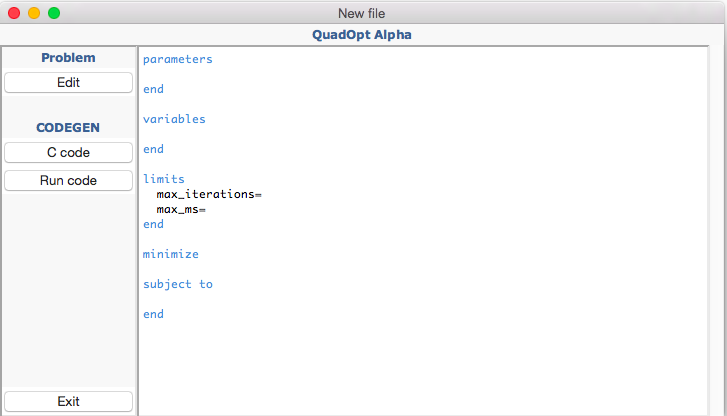
\includegraphics[scale=0.58]{grafik/QuadOptGUI}}
\caption{QuadOpt GUI}
\label{fig:quadoptgui}
\end{figure}
GUI:t skapades med hjälp av språket Python och tkinter. Anledningen till att språket Python användes var för att alla i kandidatgruppen har erfarenhet av språket samt att språket är plattformsoberoende. Visserligen är Java också ett plattformsoberoende språk som det diskuterades om att använda, men alla i kandidatgruppen hade inte erfarenhet av språket och valet föll på Python.
\newline
\newline
Tkinter är ett grafiskt bibliotek, dvs ett bibliotek som hjälper till att forma ett GUI. Anledningen till att Tkinter användes var för att det är lätt att använda och det är ett standardbibliotek som är det mest använda inom Python.
\newline
\newline
Parsern ska tolka indata från användaren och transformera indatan till ett uttryck av matriser som QuadOpt sedan kan lösa. Syntaxen för hur man skriver in ett problem har baserats på en syntax som CVXGEN använder sig av. CVXGEN är en mjukvara som specialiserar sig i att lösa diverse optimeringsproblem \cite{cvxgen}. Anledningen till att denna syntax har valts är därför att kunden har erfarenhet av den.
 
\subsection{Lösaren i MATLAB}
För att kalla på lösaren från MATLAB användes MEX. Mexfunktionen från figur~\ref{fig:mex} användes i en C fil som döptes till ''quadopt''. I denna fil fanns matrisbiblioteket och vår lösare importerad. Först görs alla inskickade MATLAB-matriser om till matriser från matrisbiblioteket genom att iterera över ''prhs[]'' och skicka MATLAB-matrisernas rader och kolumner till ''create\_matrix''. De konverterade matriserna läggs i problemstrukten och skickas till lösaren. Den resulterande matrisen konverteras till en MATLAB-matris och läggs i ''plhs[0]'' se \ref{sec:mex}.

\subsection{Utvecklingsmetod}
Under projektets gång har det inte funnits någon uppenbar utvecklingsmetodik som kandidatgruppen har följt. Inledningsvis i projektet diskuterades att vissa egenskaper från någon utvecklingsmetodik skulle följas, detta tas upp i \ref{sec:forstudie}. När iteration 1 påbörjades fanns det ingen självklar utvecklingsmetodik som följdes, men växte fram under projektets gång och detta tas upp i \ref{sec:resterande}.
\newline
\newline
För att sammanfatta hur kandidatgruppen arbetade, så  inleddes en normal arbetsvecka med möte för att stämma av hur det går för alla i gruppen, om de har förekommit några problem och vad som bör göras härnäst. För att sedan arbeta med de ''practices'' från ''eXtreme programming'' och fullfölja de aktiviteter som satts upp under förstudien. 
\newline
\newline%
Kandidatgruppen har även haft en egen hemsida som innehåller en kalender och i denna kalender brukar möten och arbetspass bokas in så medlemmar kan strukturera upp hur deras vecka ser ut.

\subsubsection{Förstudien}
\label{sec:forstudie}
Under förstudien i detta kandidatprojekt var gruppmedlemmarna överens om att någon sorts utvecklingsmetodik skulle finnas till hands. Det mest naturliga valet var att använda sig av utvecklingsmetodiken ''Scrum'', då flertalet medlemmar i gruppen har tidigare erfarenhet av den. 
\newline
\newline
Planen var att inte att använda sig av alla delmoment som ''Scrum'' har att erbjuda, utan att plocka ut de bästa delmomenten, då vissa delmoment kan kännas lite överflödiga. Den viktigaste delmomenten som hade beräknats att ta med från ''Scrum'' var det så kallade ''Scrum table''. Under varje kategori skulle sedan ett antal aktiviteter finnas med. Dessa aktiviteter skulle känneteckna det som behövdes göras för att projektet skulle bli klart. Varje aktivitet hade en tidsstämpel som antydde hur lång tid det bör ta att utföra aktiviteten. Ett exempel kan vara att en person ser att aktiviteten ''Implementera matrisaritmetik'' finns under kategorien ''Ej påbörjade''. Den aktiviteten har en tidsstämpel på 20 timmar, dvs det beräknas ta 20 timmar att implementera matrisaritmetik. Om personen vill arbeta med denna aktivitet skulle han/hon flytta denna aktiviteten till kategorien ''Under arbete'' för att sedan flytta den till ''Klart'' när aktiviteten är klar. Antalet timmar för varje aktivitet bestämdes genom diskussion, men främst gissningar då gruppen inte hade tidigare erfarenhet av någon av dessa aktiviteter sen tidigare.
\newline
\newline
Den andra attributen som hade planerats ta med från ''Scrum'' var ett ''Burn down chart''. Detta är lätt att implementera då tavlan nämnd tidigare skulle ge överblick på timmar på ett strukturerat sätt. 
\newline
\newline
Detta var alltså planen, att implementera en variant av ''Scrum'' med huvudattribut ''Scrum table'' och ''Burn down chart''. För att implementera detta användes ett antal mjukvaruapplikationer. Den första applikationen som användes var ''Trac'', en webbapplikation som används för utveckling av mjukvaruprojekt. ''Trac'' hade de attribut som ''Scrum table'' och ''Burn down chart'', men det var  inget lätt system att förstå och omständigt att konfigurera. Ingen i kandidatgruppen ansåg att ''Trac'' var tillräckligt bra och värt att lägga ytterligare tid på, därav användes inte det. Sedan gavs ''Trello'' en chans, ''Trello'' är också en webbapplikation, men dess huvudsyfte är att visa ett ''Scrum table''. Aktiviteterna i ''Trello'' gick inte att lägga timmar på och ett ''Burn down chart'' fanns inte heller tillgängligt, åtminstone inte utan använda sig av externa program. Medlemmarna i kandidatgruppen installerade externa program för att få dessa funktioner att fungera, men precis som med ''Trac'' kändes systemet för alldeles krångligt och inte heller värt att lägga tid på. Se figur \ref{fig:trello} för en bild på hur ''Trello'' såg ut för kandidatgruppen. Under en period övervägde även kandidatgruppen om en vanlig whiteboard-tavla skulle fungera, men en sådan tavla fanns ej att tillgå.

\begin{figure}[H]
\centerline{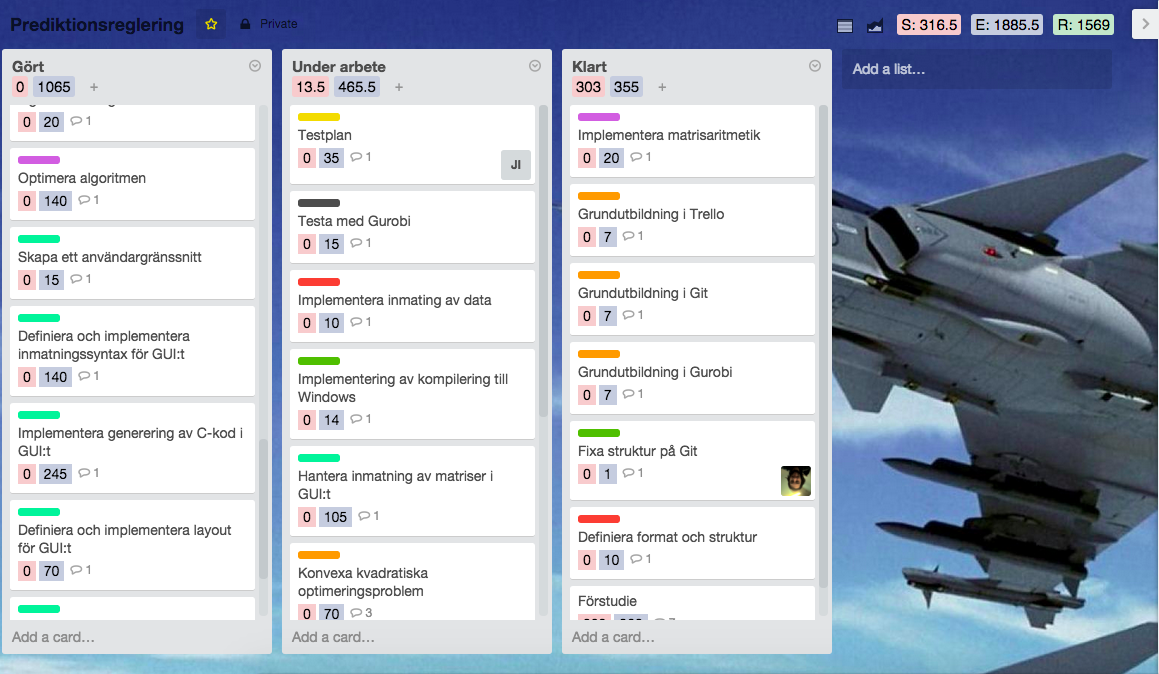
\includegraphics[scale=0.35]{grafik/trello}}
\caption{Scrum table i Trello}
\label{fig:trello}
\end{figure}

\noindent Efter dessa försök med ''Trac'' och ''Trello'' gav kandidatgruppen upp med tanken av att använda utvecklingsmetodiken ''Scrum'' och inledde första iterationen av projektet utan någon specifik utvecklingsmetodik.

\subsubsection{Resterande iterationer}
\label{sec:resterande}
Som nämnt gick kandidatgruppen in i första iterationen utan någon specifik utvecklingsmetodik, men under arbetetsgången växte en sorts utvecklingsmetodik fram.
\newline
\newline
Under projektet arbetade samtliga gruppmedlemmar i närheten av varandra. I ett tidigt skede hade kandidatgruppen tillgång till ett kontor där arbetet kunde genomföras samt möten kunde hållas. Genom att arbeta så nära varandra underlättade det att hjälpa till där det behövdes och om ett problem uppstod kunde det snabbt tas itu med.
\newline
\newline
Den utvecklingsmetodik som växte fram för kandidatgruppen liknar utvecklingsmetodiken ''extreme programming'' och de metoder som använts från den är: 
\begin{itemize}
  \item \textbf{Parprogramming} - I kandidatgruppen har vissa medlemmar parprogrammerat. 
  \item \textbf{Refactoring} - Detta har varit en stor del av projektet då kunden har tryckt på att kod ska vara väldokumenterad och strukturerad.
  \item \textbf{Continuous integeration} - ''Continuous integration'' eller CI som det brukar kallas har också varit en stor del av kandidatprojektet. Det är väldigt viktigt att all kod som skrivs fungerar med de olika komponenterna i detta projekt, t.ex. att matrisbiblioteket och koden för lösaren fungerar tillsammans. Det som har gjorts i projektet är att tester skrivs för de allra viktigaste funktioner och dessa testas kontinuerligt genom att använda ''Travis CI''. ''Travis CI'' kompilerar all kod och rapporterar om vilka tester som lyckas eller misslyckas.
\end{itemize}
Med hjälp av dessa metoder och god kommunikation mellan gruppmedlemmarna kunde projektet genomföras. 

\subsubsection{Alpha State Cards}
Under kandidatprojektet har Alpha States använts i form av Alpha State Cards. På korten finns alla faser och de krav som ska vara uppfyllda för just den fasen. Genom att checka av vilka krav som är uppfyllda för vilken fas kan gruppen få ökad förståelse för vilket tillstånd projektet befinner sig i.  

\subsubsection{Utvecklingsverktyg}
De verktygen som användes under detta kandidatprojekt var främst
\newline
\newline
\textbf{Virtuell maskin.} Till kandidatgruppens förfogande fanns en virtuell maskin med 8 GB hårddisk, 1 GB RAM och 1 GB swap. Den kör Debian GNU/Linux Stable (Wheezy) \citep{wheezy}. Maskinen används främst för att driva kandidatgruppens hemsida. Hemsidan består av nyttiga länkar och en kalender som i sin tur består av möten och grupparbeten som gruppmedlemmar bör medverka i.
\newline
\newline 
\textbf{Git.} Git är ett versionshanteringssystem. Ett versionshanteringssystem möjliggör gör parallell utveckling och tillhandahåller versioner av ens projekt i linjär tid \citep{git}. Med hjälp av Git har kandidatgruppen kunnat arbeta parallellt med stora delar av kod samt tillåtit individer att arbeta med experimentell kod.
\newline
\newline 
\textbf{GitHub.} GitHub är ett webbhotell som använder Git. Här kan man lagra alla versioner av sin kod \citep{github}. Kandidatgruppen lagrar alla väsentligt dokumentation för projektet på GitHub, dvs alla dokument som skrivs och all kod. Kandidatgruppens GitHub är dessutom privat så bara folk som ska ha med dokumentationen att göra har tillgång till sidan.
\newline
\newline
\textbf{Byggsystem.} Ett byggsystem av kandidatgruppen har skapats och gruppen klassar det som ett utvecklingsverktyg. Byggsystemet kompilerar all kod och kör alla tester som finns i biblioteket. Detta har underlättat arbetsprocessen enormt, då efter man har skrivit kod kan man helt enkelt skriva in make i terminalen och då kompileras allt och alla tester. Byggsystem är utvecklat i språket Make.
\newline
\newline 
\textbf{Travis CI.} Travis CI är en byggserver som används tillsammans med GitHub. Det Travis gör är att kalla på byggsystemet som sedan kompilerar all kod och kör testfilerna. \citep{travisinfo} 
Travis rapporterar om koden är kompilerbar eller ej, om den är kompilerbar så kör Travis alla tester som finns och rapporterar vilka tester som lyckas och misslyckas. Om Travis inte skulle ha lyckats kompilera koden eller klara alla tester så ändrar Travis statusen på projektet till ''build failing'' vilket visas på kandidatgruppens GitHub-sida. Om den klara allt så visar den ''build passing''. Den som lägger upp ny kod och orsakar en ''build failing'' får ett e-mail om att koden som har lagts upp inte är okej.
\newline
\newline
\textbf{Valgrind.} Lösaren allokerar mycket minne och då den är implementerad i C så måste man själv se till att frigöra allt minne. För att vara säkra på att det inte fanns några minnesläckor så användes Valgrind, som kan hitta minnesläckor genom ett enkelt anrop \citep{valgrind}. Hittades några minnesläckor så åtgärdades dessa.
\newline
\newline
\textbf{Emacs}. Under projektet användes ett flertal olika editorer för att skriva kod. En av dem var emacs som är en textredigerare skapad Richard 	Stallman \citep{emacs}. Vissa i kandidatgruppen använde emacs då de uppskattade att man enkelt kan arbete med flera filer vid sidan om varandra samt lättheten att byta mellan filer.
\newline
\newline
\textbf{Sublime Text.} Sublime är en annan textredigerare som vissa i gruppen använde. Det som är utmärkande drag för Sublime är att redigeraren har en rätt så unik syntax-highlighting, dvs hur den belyser text \citep{sublime}. Detta uppskattades samt att inlärningsprocessen var enkel.
\newline
\newline
\textbf{Eclipse.} Eclipse är ingen texteditor utan en IDE, dvs en integrerad utvecklingsmiljö. Den innehåller en textredigerare, kompilator och debugger. \citep{eclipse} De som använde Eclipse tyckte att debuggern kom tillhands väldigt ofta och därför använde de Eclipse.
\newline
\newline
\textbf{MATLAB.} MATLAB är ett datorprogram och programspråk som främst används för tekniska beräkningar och matematiska \citep{matlab}. Eftersom optimeringsalgoritmen som skrevs skulle kunna användas i MATLAB har MATLAB varit ett viktigt verktyg för kandidatgruppen. Tester av gruppens optimeringsalgoritm har gjorts i MATLAB många gånger. Även MATLABs matrisoperationer har varit till stor nytta för kandidatgruppen för att underlätta räkning av uppgifter. MATLAB har även en egen optimeringslösare som liknar kandidatgruppens, jämförelser har gjorts med den vid ett flertal tillfällen.
\newline
\newline
\textbf{Gurobi.} Gurobi är ett kommersiellt programverktyg som specialiserar sig att lösa optimeringsproblem utav olika sorters optimeringsproblem \citep{gurobi}. Kandidatgruppen hade i början ett krav på att vara likvärdig med Gurobi gällande hastighet.
\newline
\newline
\textbf{CVXGEN.} CVXGEN är en webbaserad applikation som genererar kod för att lösa olika sorters optimeringsproblem \cite{cvxgen}. Problemen som skall lösas ges utav av användaren via matematiska uttryck. Kandidatgruppen har använt CVXGEN då kunden är familjär med dess syntax och QuadOpt försöker efterlikna denna syntax. 
\newline
\newline
\textbf{Texmaker.} Texmaker är en textredigerare för att skriva i språket \LaTeX \hspace{0.2mm} \citep{texmaker}. Alla de dokument som har skrivits under kandidatprojektet har skrivits i {\LaTeX} och då har Texmaker varit till stor hjälp. Anledning till att många i kandidatgruppen har använt Texmaker är för att de fungerar på individernas operativsystem.
\newline
\newline
\textbf{Gummi.} Gummi är också en textredigerare för att skriva i språket {\LaTeX} men finns enbart för Linux system \citep{gummi}. Gummi kan anses vara ett lättviktigare program än Texmaker som är lite tyngre och har funktioner som inte har varit så nödvändiga.
\newline
\newline
\textbf{Google Drive.} Google Drive har använts under projektets gång för att arbete med dokument med mindre betydelse. Dokument som mötesrapporter och tidsrapporter som enbart är menat för kandidatgruppen och handledare. Vid presentationstillfällen har Google Drive också varit till nytta för att göra presentationer.
\newline
\newline
\textbf{Time Profiler.} Time Profiler är ett verktyg som finns förinstallerad på Mac-datorer. Verktyget kan visa hur mycket tid som spenderas på funktioner i ett program \citep{timeprofiler}. Då optimeringsalgoritmen som har skapats ska ta så lite tid som möjligt har detta verktyg kommit tillhands för att se hur mycket tid algoritmen spenderar i vissa funktioner. Genom att hitta de funktioner som tar mest tid att utföra har kandidatgruppen kunnat snabba upp dem någorlunda.
\newline
\newline
\textbf{DDD.} Data Display Debugger har använts i projektet för att hitta kritiska fel. Felsökningen av kod sker i ett grafiskt användargränssnitt och är ett väldigt kraftfullt verktyg \citep{ddd}.
\newline
\newline
\textbf{Doxygen.} Doxygen är en dokumentationsgenerator för programvara \citep{Doxygen}. Programmet fungerar genom att användaren har skrivit kommenterar i koden under projektets gång och då använder Doxygen sig av dessa kommentarer för att generera ett dokument. Resultaten blir en pdf som består av förklaringar för funktioner och datastrukturer. 

\subsection{Forskningsmetod}
Som tidigare nämnt var det tre olika algoritmer som var aktuella för projektet och som alla fanns med och beskrevs i boken \emph{Numerical Optimization} \citep{numericaloptimization}. Detta avsnitt kommer behandla hur algoritmerna jämfördes mot varandra för att slutligen avgöra vilken som skulle användas.
\newline
\newline
De tre algoritmerna som fanns var \emph{Active set method}, \emph{Gradient Projection method} och \emph{Interior point method}. Dessa algoritmer hade sina egna styrkor och svagheter, och det var just dessa som behövde jämföras utifrån prediktionsregleringsproblemets behov.

\subsubsection{Faktorer}
För att kunna avgöra vilken av algoritmerna som var den bäst lämpade för optimeringsproblemet, så behövdes det ett antal faktorer att jämföra dem emot.

\paragraph{Implementerbarhet}
Olika faktorer som spelade in var bland annat och möjligen det viktigaste implementerbarhet, mest eftersom projektet är väldigt tidsbegränsat och det finns ingen möjlighet till att överskrida tidsbudgeten. Eftersom det även var ett krav att lösaren skulle implementeras i C så var man tvungen att se vilka olika möjligheter för implementering som fanns där.

\paragraph{Hastighet}
Hastighet var även en väldigt viktig faktor, just på grund av att ett av de få krav som kandidatgruppen faktiskt hade var att programmet skulle vara lika snabbt eller snabbare än det kommersiella programmet Gurobi som används för att lösa alla möjliga sorters optimeringsproblem. En fördel kandidatgruppen hade gentemot Gurobi var att vår lösaren kunde optimeras för just detta problem och behövde inte vara lika generell som Gurobi.

\paragraph{Skalbarhet}
En annan viktig faktor som var avgörande var skalbarhet. Matrisernas storlekar på problemet som ska lösas kan vara uppemot flera hundra element i båda dimensionerna, därför var det väldigt viktigt att algoritmen hade en tidskomplexitet som inte var allt för stor. Just i början kan detta vara väldigt svårt att veta eftersom det inte finns så stora möjligheter till att testa större problem, utan dessa kan endast testas i ett senare skede när lösaren verkligen kommit så långt att den kan hantera dem.

\paragraph{Komplexitet}
Algoritmerna i sig kan verka vara väldigt snabba och skalbara men kan kräva en massa andra extra förkunskaper för att man ska kunna förstå sig på dem, och som skulle ta alldeles för lång tid för att läsa in inom projektets tidsbudget. Detta hänger delvis ihop med implementerbarhet, eftersom båda har med algoritmens svårighetsgrad att göra.

\paragraph{Stabilitet}
Klarar algoritmen alla olika fall av indata. Vad händer vid till exempel nollfall? Kan man lita på att algoritmen alltid kommer fram till en lösning inom rimlig tid. Hur mycket minne förbrukar algoritmen i förhållande till problemets storlek? %Behöver algoritmen någon data som räknas ut på annat vis för att fungera som den ska?

\subsubsection{Algoritmernas för- och nackdelar}
De tre algoritmerna är specialiserade på kvadratisk optimering. Men skiljer sig en del emot hur snabba de är för olika storlekar på problemen.

\paragraph{Active set method}
Det är den äldsta och standardmetoden, den är inte den snabbaste av algoritmerna, men den är lättast att implementera. Numerical Optimization boken hade även ett exempel i pseudokod för implementation av algoritmen. Den är relativt snabb upp till medelstora problem och en pålitlig algoritm.

\paragraph{Gradient Projection method}
Fungerar som Active set metoden, men istället för att bara kunna byta ett villkor åt gången till den aktiva mängden, så kan denna algoritmen byta ett flertal på en gång för att öka hastigheten. Denna algoritm är dock svårare att implementera och kräver mer förkunskaper.

\paragraph{Interior point method}
Interior point är en ganska modern algoritm och även en utav de snabbaste, den är dock mycket svårare att förstå sig på än t.ex. Active set och boken saknade implementationsexempel för denna. Har man dock mer tid på sig och ska lösa större problem är det den här algoritmen man bör välja.

\subsubsection{Slutsats om algoritmerna}
Just på grund av det problemet som kandidatgruppen skulle lösa och tidsbegränsningen som projektet hade, så ansåg gruppen att \emph{Active set} metoden lämpade sig bäst. Den hade även som tidigare förklarat en färdig pseudokodsimplementation i boken som kandidatgruppen kunde utgå ifrån.


\section{Resultat}

De frågeställningar som ställdes i början av dokumentet var:
\begin{enumerate}
\item Går det att implementera en kvadratisk optimeringslösare i programspråket C?
\item Kan kandidatgruppen implementera ett system som löser kvadratiska optimeringsproblem snabbare än Gurobi?
\item Kan projektet utföras utan någon speciell utvecklingsmetodik? 
\end{enumerate}

Svaren på dessa frågor besvaras i listan nedan:
\begin{enumerate}
\item Ja, det går att implementera en kvadratisk optimeringslösare i programspråket C med den tid som hade getts. Den kvadratiska optimeringslösaren som skrevs i programspråket C var Active set metoden. I figur \ref{fig:arkitektur} visas en överblick hur hela systemet såg ut. Där solution.c skapar en struct innehållande de matriser som problemet består av och sedan löser solvern detta problem.

\begin{figure}[h]
\centerline{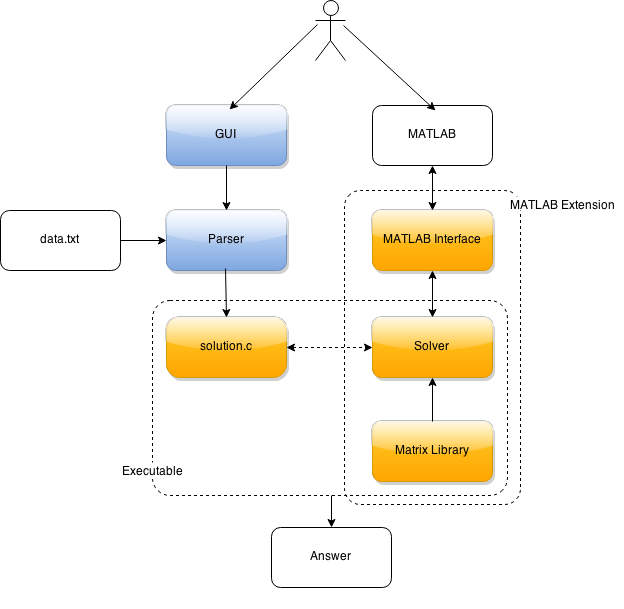
\includegraphics[scale=0.5]{grafik/arkitektur}}
\caption{Grafisk representation av lösningen}
\label{fig:arkitektur}
\end{figure}

\item Nej, ett system som kan lösa kvadratiska optimeringsproblem snabbare än Gurobi kan inte utvecklas med den tid som har funnits till hands. Kandidatgruppens sju medlemmar hade 270 timmar var att fördela projektet på, varav många timmar lades ner på dokumentation och diverse seminarier. Utan dokumentation och seminarier skulle optimeringsalgoritmen kunnat blivit bättre.

\item Ja, projektet kan utföras utan någon konkret utvecklingsmetodik. Däremot så kan man arbeta efter en viss utvecklingsmetodik utan att veta om det, dvs en skräddarsydd utvecklingsmetodik. Kandidatgruppen i detta fall gick in i iterationerna utan en utvecklingsmetodik, men under arbetsgången skapades en sorts utvecklingsmetodik som hjälpte till att utveckla optimeringsalgoritmen.
\end{enumerate}
	
	
\subsection{Kandidatgruppens gemensamma erfarenheter}
En lärdom kandidatgruppen tagit under projektets gång är vikten av att hålla regelbundna möten med kunden i början av projektet för att klargöra vad som verkligen ska göras. Många frågor uppkommer och utan en tydlig kravspecifikation blir det svårt att planera projektet. Den första kravspecifikationen som togs fram var bristfällig då gruppmedlemmarna saknade praktisk erfarenhet av dels kvadratiska optimeringsproblem och dels metodiker för programvaruutveckling. Om fler kundmöten hade planerats hade åtminstone det förstnämnda blivit ett mindre problem. Istället blev det mycket osäkerheter kring uppgiften i början av projektet vilket ledde till att kandidatgruppen förlorade tid. Till exempel försöktes lösningsalgoritmen implementeras utan tillräcklig kunskap vilket gjorde att den behövde revideras flera gånger.
\newline
\newline
Kandidatgruppen har haft goda erfarenheter med att använda molntjänster som GitHub och Google Drive för hantering av kod och dokumentation, så länge kandidatgruppen gör upp vilka som skriver vad för att undvika konflikter i versionshanteringen. När konflikter har uppstått har de tacklats med utbildning av kandidatgruppens samtliga medlemmar, vilket har lett till mer kunskapsspridning.
\newline
\newline
Till yttermera visso har kandidatgruppen fått en djupare förståelse för programspråket C. Då ett krav på programvaran är att den ska gå att kompilera och exekvera på ett flertal plattformar, har kandidatgruppen fått en insikt om vad ''implementation defined'' verkligen betyder. Det har hänt flera gånger att programmet går att exekvera på en plattform men får segmenteringsfel på en annan. Detta beror ofta på att olika operativsystem och kompilatorer hanterar minnesallokering på olika sätt.
\newline
\newline
Utöver detta har kandidatgruppen insett vikten av testning och kontinuerlig integration. Tack vare att ett synnerligen välfungerande byggsystem implementerades tidigt i projektets gång har mycket tid sparats in som antagligen skulle lagts på kompilering och felsökande. Kandidatgruppens byggserver kör automatiskt tester direkt när kod har skickats till den centrala versionshanteringsservern och varnar syndaren via elektronisk post om något test eller kompilering skulle misslyckas. Detta har gjort att fel har upptäckts tidigt och åtgärdats snabbt.

\subsection{Översikt över de individuella utredningarna}
I de individuella utredningarna har kandidatgruppen rapporter som behandlar: 
\begin{itemize}
	\item En undersökning av olika byggsystem.
	\item Hur man är en bra team ledare och vad best practices är.
	\item Optimering av matrisbibliotek. 
	\item {\LaTeX} i ett programmeringsprojekt.
	\item Testning av mjukvara. 
	\item Hur man tar fram en bra arkitektur. 
	\item Kvalitetssäkring i ett projekt.  
\end{itemize}
Dessa individuella delar bygger på antingen författarens roll eller ett område författaren ägnat mycket av sin tid åt under projektets gång. I de fall där den individuella delen baseras på en roll har författaren valt att rikta in sig på en specifik del av rollen som är kopplad till projektet. De resterande områden som skrivits om har inte enbart varit ett område där författaren lagt mycket utav sin tid utan det är även områden som projektet har gynnats mycket av.

\section{Diskussion}
Under denna del kommer en diskussion angående om resultaten ske samt metoderna som användes.

\subsection{Resultat}
Resultaten måste anses vara rimliga. Den första frågeställningen ställer frågan om det går att implementera en kvadratiska optimeringslösare i programspråket C med den tid som har getts. Resultatet visar att det går att implementera en sådan lösare i språket C givet den tiden som har getts. Något att ta hänsyn till däremot är att en bättre lösare skulle kunnat produceras med mer tid. Med mer tid skulle kandidatgruppen kunnat ha implementerad flera olika sorters lösningsmetoder i den kvadratiska optimeringslösare. Kandidatgruppen valde att implementera Active set metoden, med mer tid skulle andra sorters metoder kunnat implementeras, ett exempel är Interior point metoden. 
\newline
\newline
Anledningen till att algoritmen går att implementera i C är för att C är ett turingkomplett språk, dvs ett språk som kan beräkna samtliga beräkningsbara problem i det, givet tillräcklig tid och tillräckligt minnesutrymme. Språket C arbetar också väldigt nära hårdvaran, vilket i sin tur gör att koden som har skrivits av kandidatgruppen kan exekvera snabbare än vad den skulle göra i andra språk. Det enda kandidatgruppen saknade i språket C var att kunna överlagra operatorer. Med hjälp av att kunna överlagra operatorer skulle t.ex. matrismultiplikationer ske med ett enkelt gånger-tecken istället för att göra ett funktionsanrop. Detta skulle ha kunnat medföra enklare kod, som i sin tur kan vara lättare att underhålla. 
\newline
\newline
Den andra frågeställningen kandidatgruppen hade var om QuadOpt skulle kunna lösa kvadratiska optimeringsproblem snabbare än Gurobi. Svaret vart nej. Anledningen till detta är att Gurobi är en kommersiell programvara som har arbetats med under en väldigt lång tid av välbetalda utvecklare och konsulter. Medan QuadOpt inte har haft samma förutsättningar. Kandidatgruppen skulle förutom att skapa en optimeringsalgoritm också skapa ett GUI och en parser i Python. Dessutom skulle kandidatgruppen även delta i diverse olika entreprenörskapskurser, förbereda opponeringar och skriva en massa dokument. Det ska också tilläggas att kandidatgruppen gjorde ett eget matrisbibliotek. Detta tog upp mycket av tiden som fanns för kandidatprojektet. Om några av dessa moment inte fanns med skulle kandidatgruppen kunna lagt dessa timmar på optimeringsalgoritmen och möjligtvis kunna matcha Gurobis hastighet.
\newline
\newline
Den sista frågeställningen kandidatgruppen hade var om man kunde utföra projektet utan någon speciell utvecklingsmetodik. Denna frågeställning är nog den svåraste att ge ett konkret svar på. Kandidatgruppen svarade ja, det går att gå in i ett projekt utan någon speciell utvecklingsmetodik. Däremot när man väl arbetar med ett projekt utvecklas en sorts utvecklingsmetodik, även om man inte är medveten om det. I kandidatgruppens fall användes attribut från metodiken ''Extreme programming'' till viss del. Attribut som parprogrammering, refaktorering och kontinuerlig integration.

\subsection{Metod}
Valet av kvadratisk optimeringsalgoritm kan ses som aningen naiv. Hade kandidatgruppen dock haft mer kunskap om ämnet hade kandidatgruppen kunnat resonerat mer kring vilken algoritm som skulle använts och vägt för- och nackdelar mellan dessa. Huvudanledning till att valet föll för Active set metoden är för att kunden rekommenderade den, men kunden sa också åt kandidatgruppen att undersöka de andra algoritmerna. I efterhand tror kandidatgruppen att Interior point metoden skulle varit lättare att utföra i C-kod och dessutom lösa problemet snabbare än vad Active set metoden gör. Visserligen vet inte kandidatgruppen vilka problem som skulle kunna uppkomma om man skulle implementera Interior point och frågan om vilket val som är rätt endast kan besvaras genom att implementera alla de tre metoderna som jämfördes i början för att sedan ta ett beslut.
\newline
\newline
Att implementera ett matrisbibliotek är något som kandidatgruppen valde att göra för att de biblioteken som fanns tillhands var alldeles för svåra att begripa. Valet av att implementera ett matrisbibliotek var inget som var planerat under förstudien och detta tog väldigt många timmar att implementera samt att testa. Kandidatgruppen är nöjda med valet av att implementera ett eget matrisbibliotek, mycket på grund av att man vet vad som finns och hur det fungerar. De som sedan tar över projektet utvidga biblioteket hur mycket de vill.
\newline
\newline
Kandidatgruppen hade kontakt med kunden främst genom e-mail och träffades vid enstaka möten. Relationen mellan kandidatgruppen och kunden har varit bra och inga problem har dykt upp. Kandidatgruppen skulle möjligtvis kunnat ha visat kunden arbetet som har gjorts vid flera tillfällen. 
\newline
\newline
Valet av att gå in i iterationer utan en utvecklingsmetodik är inget kandidatgruppen ångrar. Som tidigare nämnt kan en kandidatgrupp arbetat på ett visst sätt som liknar en utvecklingsmetodik utan att veta om det. I detta fall ledde ledde arbetssättet till en variant av utvecklingsmetodiken eXtreme programming.

\subsection{Arbetet i ett vidare sammanhang}
Utöver att projektet har bidragit till vår egen och Saabs nytta kan projektet ha påverkat och ha framtida påverkan på samhället och miljön vi lever i. Mycket av informationen nedanför är hämtad direkt från Saabs hemsida och kan vara vinklad.   

\subsubsection{Etiska och samhälleliga aspekter}
Att utveckla teknik åt ett företag som förser regeringar, myndigheter och företag med militära tjänster och produkter reser många etiska frågor, till exempel: 
\begin{itemize}
\item Etiskt rätt att utveckla och sälja vapen?
\item Hur kan man förhindra att vapen och känslig information hamnar i fel händer? 
\end{itemize} 
Vapen som stridsflygplanet JAS 39 Gripen kan döda många människor och orsaka kaos i världen, varför existerar det då sådana vapen? Samhällen idag (och sedan lång tid tillbaka) har ett behov av vapen för att kunna försvara sig mot varandra, terroristgrupper och enskilda individer som av någon anledning vill attackera. Utan krig och orättvisor hade efterfrågan på Gripen saknats. I en perfekt värld hade det alltså inte existerat några vapen. Tyvärr är inte världen perfekt. 
\newline
\newline
Saabs vision med sina produkter och deras etiska riktlinjer avser att människor ska kunna känna sig säkra. Dessa riktlinjer kan dock ifrågasättas av Saabs kunder (mer om detta senare). Om vapnen inte används för att döda oskyldiga utan endast för att bidra till ett säkrare samhälle kan det ses som etiskt rätt att utveckla och sälja vapen. 
\newline
\newline   
På Saabs hemsida kan man läsa att de har policyn noll tolerans mot korruption och att det finns många åtgärder för att uppfylla detta. I figur~\ref{fig:zerotolerance} visas en grafisk överblick över deras huvudsakliga åtgärder. 
\leavevmode
\begin{figure}[h]
	\centering
	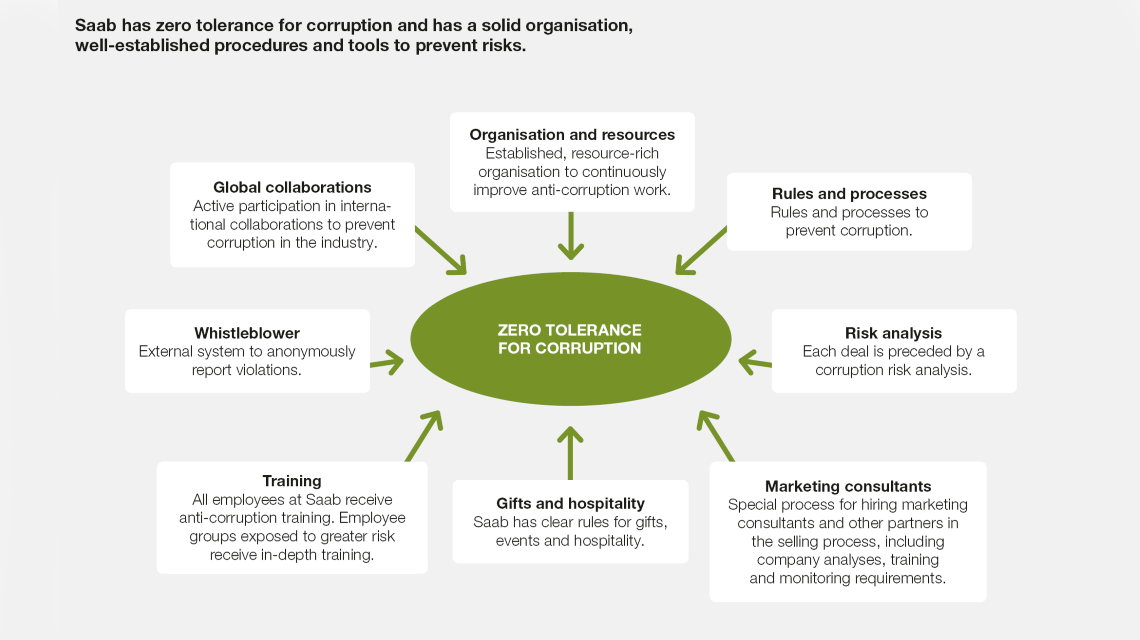
\includegraphics[scale=1.4]{grafik/modell_zero_corruption_1140x640.png}
	\caption{Modell zero corruption \citep{saabimg1}}\label{fig:zerotolerance}
\end{figure}  
\\
Till exempel gör Saab alltid riskanalyser i samband med affärer för avgöra om det finns risk för korruption. De undersöker risker med vart affären äger rum, vem köparen är, hur upphandlingen går till och hur köparen kom i kontakt med företaget. Om riskerna inte gick att eliminera eller inte var hanterbara drar sig Saab ur affären. Detta är en åtgärd för att förhindra att produkterna hamnar i fel händer. 
\newline
\newline
När utomstående parter är inblandade och flödet av pengar inte är helt under Saabs kontroll finns det alltid risker att produkterna kan hamna i fel händer. För att minimera riskerna ser Saab till att deras etiska värden och riktlinjer strikt följs av utomstående/tillfälligt anställda konsulter och partners. Dessa partners måste genomgå utbildning och skriva under att följa Saabs etiska värden och riktlinjer. I avtalen ingår det att Saab har rätt till att kontrollera om riktlinjerna verkligen följs.   
\newline
\newline
För att förhindra korruption inom företaget utbildar Saab all personal inom ämnet. De har även ett system kallat ''Whistleblower'' för att rapportera suspekta aktiviteter och som garanterar rapporterarens anonymitet.              
\newline
\newline
Utöver vapen levererar Saab bland annat system för väderstationer, minröjning och att detektera kemiska, biologiska, radioaktiva samt kärnvapen. \citep{security}

\subsubsection{Miljöaspekter}
Vårt projekt är inte en skada för miljön eftersom det endast är samling algoritmer för att lösa och visualisera optimeringsproblem.  
\newline
\newline
Om Saab skulle använda vårt projekt i jaktflygplanet JAS 39 Gripen som projektet härstammar ifrån, uppkommer frågor kring hur pass miljövänliga företaget Saab och Gripen är. På deras hemsida \citep{saabimpact} kan man läsa om deras arbete för att minska avtrycket på miljön. De har till exempel satt upp som mål att reducera deras koldioxidutsläpp från försäljningar med tjugo procent till år 2020. I figur~\ref{fig:saabkoldioxid} visas Saabs koldioxidutsläpp och deras mål.   
\leavevmode
\begin{figure}[h]
	\centering
	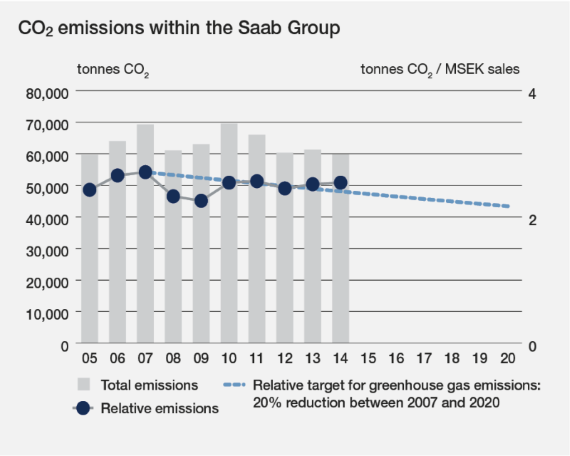
\includegraphics[scale=1.5]{grafik/saabemissions.png}
	\caption{Utsläpp koldioxid Saab \citep{saabimg2}}\label{fig:saabkoldioxid}	
\end{figure} 
\\
För att nå målet arbetar Saab med att reducera elförbrukningen på deras fabriker och utsläpp från resor vilka är de största faktorerna för deras koldioxidutsläpp. Genom att fokusera på att ändra de anställdas vanor, ny teknik och strategisk planering av fabrikerna har de lyckats sänka koldioxidutsläppen från fabrikerna med tjugo procent mellan åren 2009 och 2014. För att minska utsläppen från resor nämner Saab bland annat att de uppmuntrar resfria möten och samåkningar.
\newline
\newline 
Deras hantering av miljöfarliga ämnen möter EU's förordning REACH (Registration, Evaluation and Authorisation of Chemicals) som strävar efter att förbättra skyddet av människors hälsa och miljön från risker som kan förorsakas av kemikalier \citep{reach}. 
Saab är även kontributör till projektet Clean Sky som är det mest ambitiösa luftfartsforskningsprogrammet i Europa. Målet med Clean Sky är att utveckla ny teknik för att göra luftfarten mer miljövänlig med mindre bullriga och mer bränsleeffektiva flygplan. \citep{cleansky}     
\newline
\newline
Stridsflygplanet JAS 39 Gripen använder i dagsläget en jetmotor som drivs på fotogen. Fotogen är ett fossilt bränsle som leder till koldioxidutsläpp vid förbränning. Detta gör Gripen till ett system som bidrar till miljöförstöring. 
\newline
\newline
Det verkar som att Saab har ambitioner om att själva bli miljövänligare och att bidra till utvecklingen av miljövänligare teknik. De gör dock fortfarande ett negativt avtryck på miljön eftersom det sker utsläpp av koldioxid och de använder miljöfarliga ämnen i deras produkter. Detta kan dock ses som en direkt följd av att det idag tyvärr inte är lönsamt att använda eller existerar effektiv miljövänlig el och teknik.  
\newline
\newline
Skulle användandet av vårt projekt göra någon skillnad? Detta går tyvärr inte att svara på då kandidatgruppen saknar uppgifter på hur vår optimeringslösare skulle bidra till miljövänligheten hos stridsflygplanet JAS 39 Gripen.        

\section{Slutsatser}
De slutsatser kandidatgruppen har kommit fram till är att valet av metod till optimeringsalgoritmen inte var helt genomtänkt. Anledningen till detta är att kandidatgruppen saknade förkunskaper inom området och bör ha lagt fler timmar på utbildning inom optimeringsproblem i detta område vilket hade lett till ökad förståelse för området på ett generellt sätt vilket hade lett till att de algoritmer som varit kandidater hade kunnat bedömas på ett mer kvalificerat sätt för att kunna göra ett mer kvalificerat val. 
\newline
\newline
Kandidatgruppen ångrar inte valet av att ta med kravet att QuadOpt ska vara jämbördig med Gurobi vilket inte uppnåtts. Genom att misslyckats med detta har kandidatgruppen lärt sig förhandla krav med en kund och göra sitt yttersta för att matcha en kommersiell produkt vilket inte anses vara en enkel uppgift med tanke på den begränsade tiden kandidatgruppen haft vilket ett företag som utvecklar en produkt som Gurobi troligtvis haft större tillgång av. Dock kan man dra slutsatsen att det är möjligt att skapa en likvärdig produkt rent prestandamässigt om det funnits mer tid dels för utveckling men framför allt, som tidigare nämnts, utbildning.
\newline
\newline
Kandidatgruppen ångrar inte heller valet av att inte gå in i iterationerna utan en konkret utvecklingsmetod eftersom arbetet fungerade på ett tillfredsställande sätt utan en sådan metod.  
\section{Fortsatt arbete}
Det här projektet erbjuder många olika möjligheter till fortsatt arbete för alla inblandade parter. Detta inkluderar alla olika delar av projektet. Det fortsatta arbetet innebär till största delen att vidareutveckla dessa delar för att förbättra befintliga funktioner och eventuellt lägga till nya funktioner till det redan befintliga programmet. 
\newline \newline
Till att börja med kan det ligga i Saabs och kundens intresse att fortsätta arbeta med produkten, framför allt lösaren. Det mest relevanta för denna part skulle till exempel vara att integrera produkten med Saabs system, ARES, vilket ligger på en hög nivå i det avseendet att produkten måste vara mycket pålitlig och effektiv för att detta ska bli aktuellt. Därför går det även att se hur denna part skulle kunna anse att det är en bra idé att vidareutveckla den levererade produkten för att uppfylla de standarder och krav som finns. För denna part finns det även aspekten att arbeta vidare med produkten i ett rent akademiskt syfte för simuleringar relaterade till Simulink och MATLAB. Detta är möjligt då Saab och kunden kommer ha tillgång till all källkod som krävs för dessa typer av arbete.
\newline \newline
Vidare går det även att titta på vidare arbete ur kandidatgruppens perspektiv men den potential som finns är begränsad på grund av att produkten utvecklats åt Saab. Trots detta finns möjligheten att arbeta vidare på produkten. Det som framför allt skulle vara önskvärt att arbeta vidare med är att genomföra omfattande tester av lösaren med fler typer av testdata vilket varit problematiskt på grund av storleken på datan. För kandidatgruppen skulle fortsatt arbete även kunna innebära att den nuvarande lösaren skrivs om för att tillämpa en annan optimeringsmetod än den nuvarande. Den som i nuläget används är Active set men det är även möjligt att implementera till exempel Interior point metoden.
\newline \newline
Undersöks istället enbart produkten utan att ta hänsyn till någon av parternas perspektiv är det lättare att se möjligheter för vidareutveckling. Den del av produkten som är kopplad till MATLAB har väldigt begränsad möjlighet till vidareutveckling i och med att denna del i stort sett är en översättning av lösaren vilket gör att det istället är mer relevant att titta på lösaren vilken har stor potential att arbetas vidare med. I lösaren finns det både optimeringsmöjligheter samt möjligheten att lägga till eller ändra funktioner. När det gäller optimering kan man tänka sig att vidare arbete innebär att programmet optimeras för att vara effektivare med de tillgängliga resurserna för att på så sätt bli snabbare. De funktioner som redan finns implementerad som kan arbetas vidare med kan till exempel vara hur lösaren hittar sin startpunkt för optimeringen.
\newline \newline
De andra två delarna av programmet, det grafiska gränssnittet och parsern, har också potential att arbetas vidare med. Det är dock viktigt att poängtera att fortsatt arbete med dessa delar inte är direkt relaterade till hur lösaren fungerar eller prestandan hos denna vilket kan ses som att det är mindre värdefullt att arbeta vidare med detta jämfört med lösaren som trots allt är programmets huvudsakliga komponent.
\newline \newline
En brist som funnits under projektet har varit viss avsaknad av testfall vilket kommer av att testfallen är stora och omständiga att ta fram. Skulle det finnas tillgång till fler testfall är ytterligare tester ett område som kan arbetas vidare på. Detta kan till exempel leda till att fler områden i lösaren kan optimeras för att bli snabbare eller att eventuella brister uppdagas. Brister skulle till exempel kunna vara ovanliga specialfall som i nuläget inte har beaktats och som endast i enstaka fall kan leda till något problem.


\newpage
%start the appendix
\appendix

%\appendixpage
%\addappheadtotoc
\renewcommand{\thesection}{\arabic{section}}

%Yngves report
\addcontentsline{toc}{section}{Bilagor}
\addcontentsline{toc}{section}{\protect\numberline{A} Utvärdering av byggsystem}
\stopcontents

\startcontents[sections]
\LIPSTitelsidayngve
\setcounter{section}{0} 
\printcontents[sections]{ }{1}{}
\newpage
\section{Inledning}
Jag har gjort en filhanterar som visualiserar alla filer och mappar i 3D med hjälp av OpenGL. Inspirationen till detta projekt var bland annat FSN (File System Navigator) som gjordes av SGI för IRIX systemen och FSV(File System Visualizer) som är en remake av FSN på Linux, se figur~\ref{fig:fsn}. En annan inspiration var det lite modernare TDFSB som även visar upp bilder och filmer i 3D världen, se figur~\ref{fig:tdfsb}. 

\begin{center}
\begin{figure}[H]
    \centering
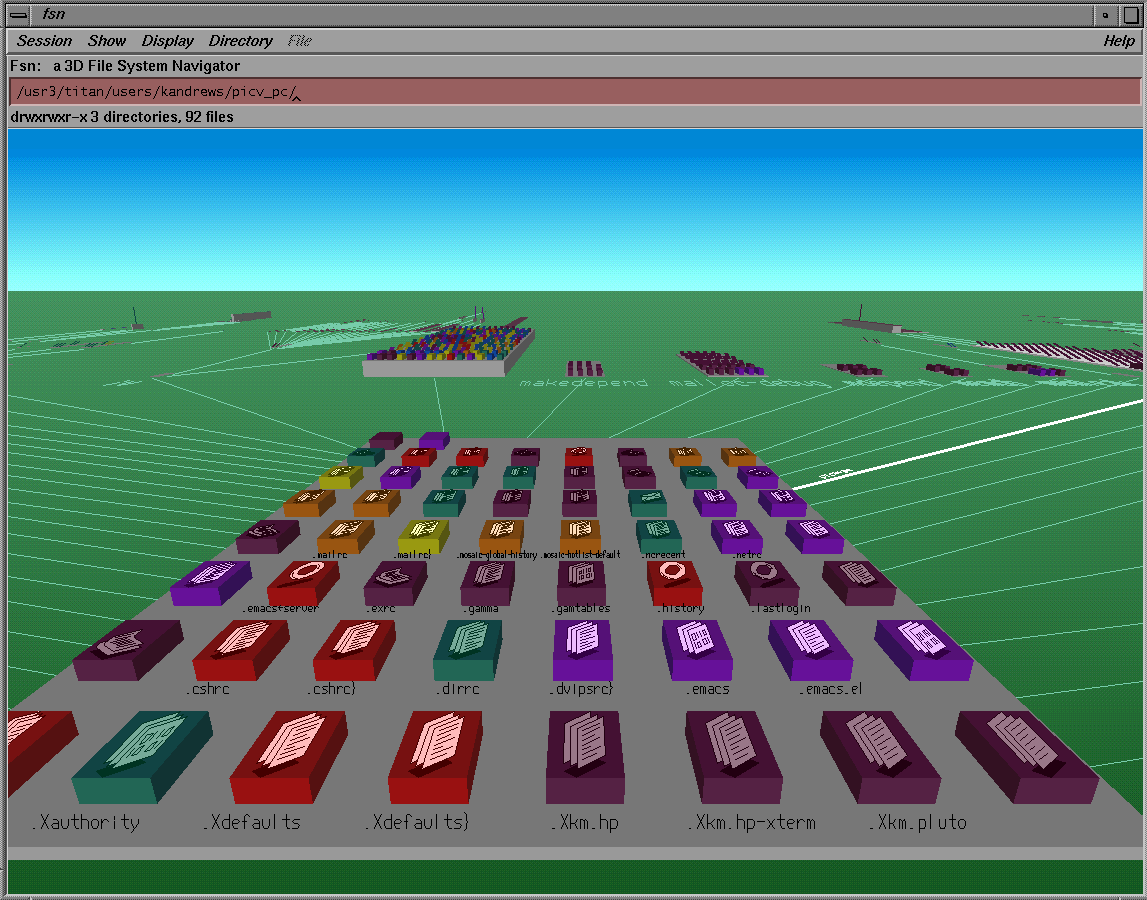
\includegraphics[width=8cm]{../grafik/fsn1.png}
\caption{FSN.}
\label{fig:fsn}
\end{figure}
\end{center}

\begin{center}
\begin{figure}[H]
    \centering
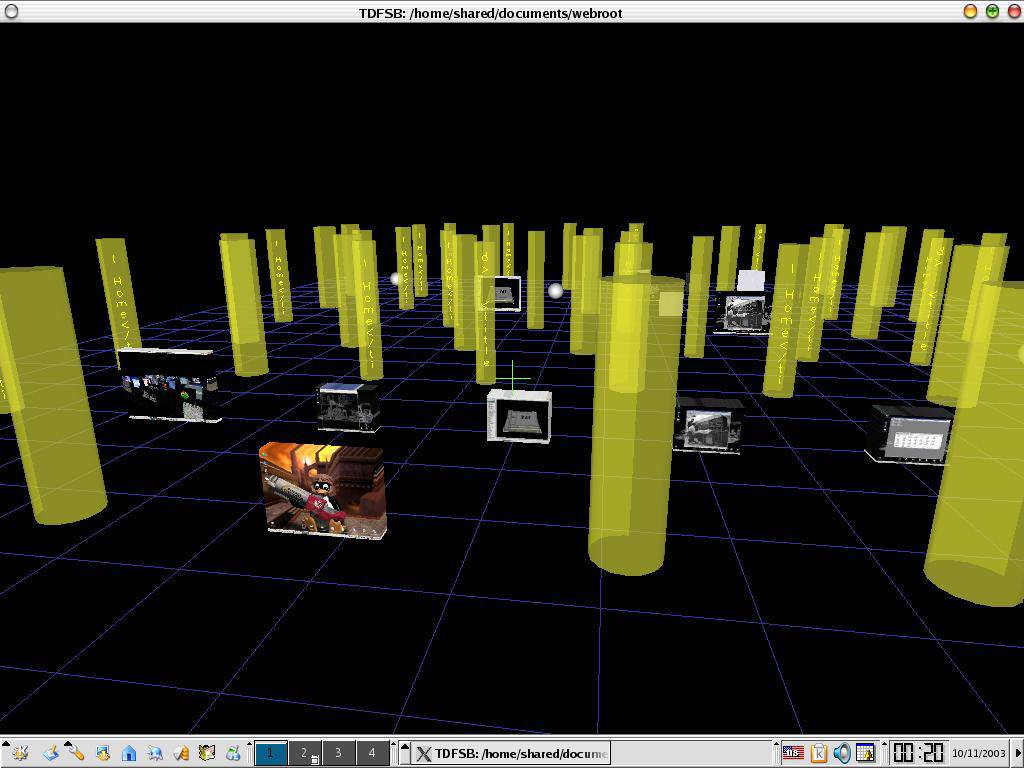
\includegraphics[width=8cm]{../grafik/tdfsb.jpg}
\caption{TDFSB.}
\label{fig:tdfsb}
\end{figure}
\end{center}

De ursprungliga obligatoriska kraven för produkten var följande:
\begin{LIPSkravlista}
\LIPSkrav{Original}{Alla filer ska representeras av block med någon textur på, är det en bild så ska bilden användas som textur}{1}

\LIPSkrav{Original}{Alla mappar ska representeras av block med någon textur}{1}
\LIPSkrav{Original}{Alla mappar och filer i en mapp ska vara placerade på en platta med en textur}{1}
\LIPSkrav{Original}{Ljussättningen ska ske med en Phong-shader}{1}
\LIPSkrav{Original}{Alla block ska ha skuggor}{1}
\LIPSkrav{Original}{Navigeringen ska vara first person där piltangenterna styr x och z koordinaterna och musen styr kameren i ett sfäriskt koordinatsystem}{1}
\LIPSkrav{Original}{Man ska inte kunna gå igenom filerna(collisions detection)}{1}
\LIPSkrav{Original}{Du ska kunna gå in i en mapp så transporteras du till den nya mappen)}{1}
\LIPSkrav{Original}{Du ska kunna klicka på en fil/mapp och få upp alla möjliga alternativ såsom radera, öppna...)}{1}
\LIPSkrav{Original}{Om du raderar en fil ska övriga filer ordna sig så det inte är några luckor någonstans}{1}
\LIPSkrav{Original}{Skydome ska finnas}{1}
\LIPSkrav{Original}{Endast Linux kommer stödjas}{1}
\end{LIPSkravlista}


och de ej obligatoriska kraven var följande:
\begin{LIPSkravlista}
\LIPSkrav{Original}{Du ska kunna få upp en terminal i filhanteraren}{2}
\LIPSkrav{Original}{Du ska kunna klicka på en mapp och sedan få upp en portal som du kan se in i mappen genom}{2}
\LIPSkrav{Original}{När du raderar en fil ska den explodera}{2}
\LIPSkrav{Original}{Innehåller en mapp många filer/mappar ska frustum culling användas för att minimera beräkningar}{2}
\LIPSkrav{Original}{Mapparnas texturer ska vara den ikon filen som operativsystemet använder med transparens, då ska renderingsordningen och vara korrekt}{2}
\end{LIPSkravlista}
Under projektets gång gick de obligatoriska kraven igenom en modifikation på grund av att projektet tog längre tid än vad jag trodde samt att en del inte riktigt passade in. Krav 5 togs bort på grund av tidsbrist, krav 6 gjordes om så att användaren bara navigerade i XZ planet då detta passade mycket bättre samt en del förenklingar kunde göras. Krav 9 togs bort då en terminal ansågs vara mycket enklare att implementera så all modifikation av filsystemet görs via den. Inga av de ej obligatorska kraven uppfylldes på grund av tidsbrist. I figur~\ref{fig:tmbtrf} kan man se resultatet. 
\begin{center}
\begin{figure}[H]
    \centering
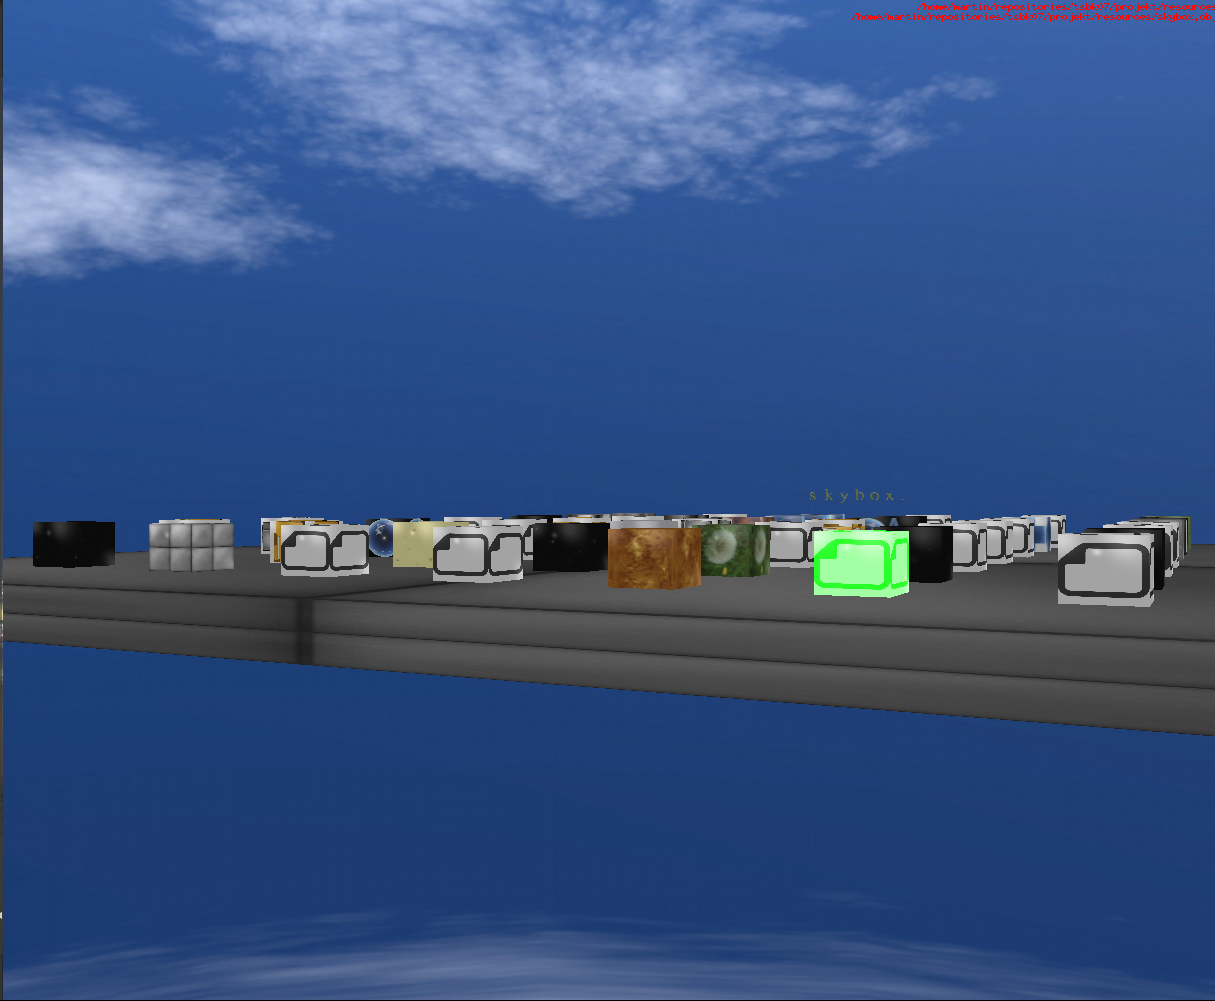
\includegraphics[width=8cm]{../grafik/tmbtrf.png}
\caption{TMBTRF.}
\label{fig:tmbtrf}
\end{figure}
\end{center}

\section{Bakgrund}
Det svåraste problemet jag hade innan jag började med projeketet var att på ett effektivt sätt interagera med datorns filsystem. Detta löstes rätt enkelt när jag upptäckte Boost::Filesystem. Detta bibliotek är inte speciellt använt så det finns inte så mycket hjälp att hitta på forum men dokumentation för det är väldigt bra så när jag väl kom in i det så fungera det väldigt bra. Funktioner såsom att byta namn och radera filer fanns redan implementerade så detta underlättade mycket.
\\
\\
Ett annat problem som var svårare än vad jag trodde var att visa filnamn i en 3D miljö. Den enklaste lösning skulle varit att använda något bibliotek för att generera texturer med en font till exempel FreeType. Jag försökte detta och jag kommer inte ihåg varför men jag fick det inte att fungera. För att få detta snyggt så skulle texturerna behöva vara transparenta så jag skulle behöva ta hänsynt till ordningen som alla objekt renderas. Min lösning på problemet var att generera .obj filer för alla tänkbara bokstäver och tecken som kan förekomma i ett filnamn. Jag valde alla bokstäver a-z och A-Z, alla siffror samt tecknen . - \_. Detta gjordes med ett python script i cad-programmet FreeCad. För att minimera inläsningstiden så läses alla dessa modeller in vid starten av programmet och återanvänds hela tiden. För att undvika problem som kan uppkomma vid långa filnamn som sträcker sig över hela miljön så visas bara de 7 första tecknen i filnamnet.
\\
\\
Anledningen till att C++ valdes var mest för dess datastrukturer såsom Vector, Map och string. Allting som kan göras i C++ kan självklart göras i C men där så är allting klart. Detta gjorde så att jag kunde göra en väldigt allmän klass som representerar alla objekt i 3D världen. Programmet arbetar också mycket med strängar och då är String väldigt mycket smidigare än en char array.
\\
\\
Ett problem som upptäcktes senare var att när man går in i en mapp som innehåller många filer, speciellt bilder, så tar det rätt lång tid innan hela världen har genererats. Detta skulle kunna lösas genom att ha en separat tråd som förbereder alla undermappar i den nuvarande mappen. Detta har dock inte implementeras men skulle jag fortsätta utveckla TMBTRF så skulle detta vara ett av de första problemen jag skulle lösa. 

\section{Teori}
I boken ''Software Product Quality Control'' \citep{SPQC} nämns ett antal definitioner som förtydligar vad kvalitetssäkring innebär, dessa syns nedan.  

\begin{itemize}
  \item ''Quality assurance: a planned and systematic pattern of all actions necessary to provide adequate confidence that an item or product conforms to established technical requirements.'' \citep[p.19]{SPQC} 
  \item ''Constructive quality assurance: All means to be used in constructing a product in a way so it meets its quality requirements.'' \citep[p.19]{SPQC} 
  \item ''Analyctical quality assurance: All means of analysing the state of the quality of a product.'' \citep[p.19]{SPQC} 
\end{itemize}
\noindent Kvalitetssäkring innebär följaktligen att man som leverantör av en produkt eller tjänst ska se till att de uppfyller de krav som har satts upp i en eventuell kravspecifikation. Det är dessa krav som sätter standarden för vad som är rätt nivå gällande kvalité. Under arbetsgången måste man analysera om man är på väg att uppfylla kraven eller inte, i sådana fall måste detta åtgärdas omedelbart.
\newline
\newline
Med detta sagt finns det flera steg i ett projekt att kvalitetssäkra. Ett effektivt sätt att göra detta på är genom att följa Shewhart cykeln, det vill säga planera, göra, studera och agera (PGSA) \citep{PDCA}. Shewhart cykeln är en iterativ fyra stegs metod, se figur \ref{fig:shewcycle}. Metoden är utvecklad av William Edwards Deming. Namnet ''Shewhart'' kommer från en av Demings kollegor \citep[p.~88]{Deming}. 
\begin{figure}[h]
\centerline{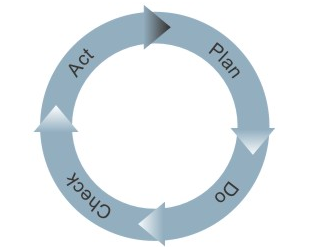
\includegraphics[scale=0.5]{ruben-tex/graphic/shewhartcycle}}
\caption{Shewhart cykeln \citep{Mindtools}}
\label{fig:shewcycle}
\end{figure}
\begin{enumerate}
  \item Planera. I detta skede ska målet fastställas, det vill säga sätta upp de krav som behövs för att kunden skall bli nöjd. Genom att göra detta är det tydligt om vad som skall göras och en överenskommelse finns mellan kund och leverantör. 
  \item Göra. När man konstaterat vad som behöver göras för att kunden skall bli nöjd är det dags att implementera ett sätt att arbeta och fullfölja processen.
  \item Studera. Efter att ha följt processen under en viss period är det dags att utvärdera om processen man har följt kommer leda till att man uppfyller de målen man har fastställt i planeringsfasen.
  \item Agera. Om man under studeringsfasen upptäcker att processen man följer inte kommer leda till att man uppfyller de krav som kund och leverantör var överens om måste detta åtgärdas omedelbart genom att planera om arbetsprocessen eller i viss mån diskutera kraven med kunden. Om processen som följs kommer uppfylla de krav som har satts upp kan man fortsätta med iterationerna av Shewhart cykeln precis som innan.
\end{enumerate}
\begin{figure}[h]
\centerline{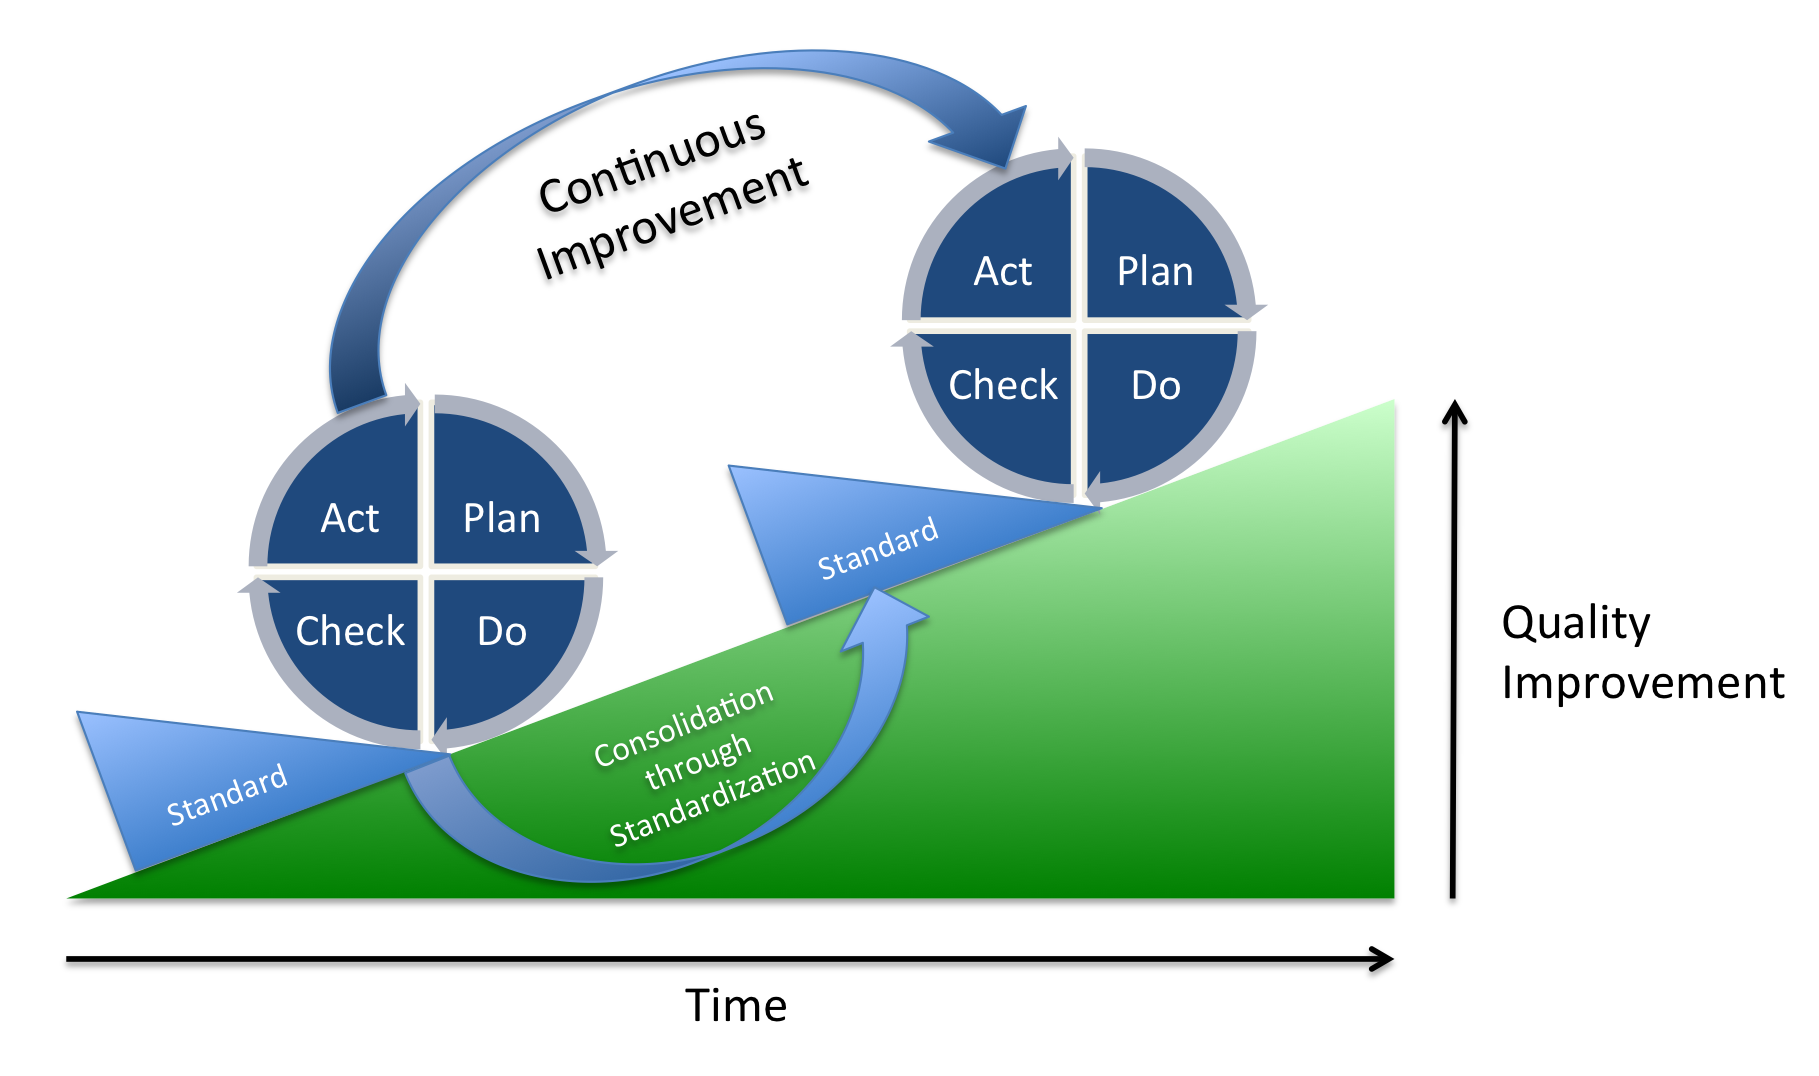
\includegraphics[scale=0.15]{ruben-tex/graphic/PDCA_Process}}
\caption{PDCA process \citep{Vietze}}
\label{fig:pdcaprocess}
\end{figure}
\noindent Genom att följa Shewhart cykeln under ett projekt kan man iterativt förbättra sin arbetsprocess och genom detta öka kvaliteten av den produkt man utvecklar, se figur \ref{fig:pdcaprocess}.
\newline
\newline
När det väl är dags för överlämning av en produkt eller tjänst är det bra att göra en kravinspektion innan. En kravinspektion enligt IEEE standarden för ''Software reviews'' syns nedan.

\begin{tcolorbox}[boxrule=1pt,leftrule=5pt,arc=0pt,auto outer arc]
\textbf{''}A process or meeting during which a software product is examined by a project personnel, managers, users, customers, user representatives, or other interested parties for comment or approval\textbf{''} \citep{SFSR}
\end{tcolorbox}

\noindent
Det man vill få gjort med en kravinspektion är alltså att produkten eller tjänsten som har tagits fram ska utvärderas av berörda parter så att den uppfyller de krav som har fastställts i ett tidigare skede för ett godkännande. En kravinspektion kan se ut som sådan \citep{Sandahl}:
\begin{enumerate}
\item{Tillträde.}
\item{Planering och översikt. Under detta steg sker en planering över hur inspektionen ska gå till och en översikt av produkten ges.}
\item{Individuell granskning. De berörda parterna granskar produkten eller tjänsten.}
\item{Möte. Efter granskningen görs en lista av alla de defekter som kan ha hittats.}
\item{Ändringar och uppföljning. I detta skede åtgärdar man de defekter som stöttes på och normalt brukar verifiera detta.}
\item{Utträde.}
\end{enumerate}

\subsection{Sammanfattning}
Sammanfattningsvis kan man konstatera att ett återkommande tema för att ta fram en högkvalitativ produkt eller tjänst är att planera, utföra och granska, för att sedan upprepa proceduren under projektets gång. Detta är dock bara en teoretisk tillämpning och verkligheten kan se annorlunda ut.

\section{Metod}
	För att ta reda på all information som behövs har ett flertal böcker blickats igenom. Ingen av dem har läst till 100\%, utan endast de intressanta delarna har läst med mer nogrannhet. För att verifiera att det som lästs stämmer har vissa delar testats i praktiken, i detta fall på projketet. Till exempel så har enhetstester körts på matris bibliotekts funktioner såsom matrisaddition, sytemtester och modultester har körts på den kvadratiska problem-lösaren och acceptanstester har körts på alla delar i projektet för att se till att alla krav är uppfyllda. Mer om detta kan läsas i resultat.
	
\subsection{Enhetstest}
	I ''Software Unit Testing'' \citep{ivv} definierar ett enhetstest som ett test på den minsta möjliga samlingen kod som fortfarande går att testa nyttofullt, alltså att koden är tillräckligt stor för att fel ska kunna uppstå. Dessa test är bra då de är riktade mot en så liten portion med kod och i och med detta sällan missar buggar och fel. Det som kan vara krångligt med enhetstest är att just hitta dessa minsta samlingarna med kod, speciellt om det är en extern part (en annan programmerare) som ska skapa och utföra testen. I och med att man kör enhetstester på så små delar av kod har de i teorin en tendens till att bli väldigt många om man ska täcka tillräckligt stor funktionalitet. Detta är dock oftast inget problem i praktiken eftersom många små funktioner ofta är triviala och har ytterst få uppgifter. Då behöver inte så många test skrivas, om ens ett enda.
\subsection{Modultest}	
	Det finns flera olika definitioner av vad en modul är, och i och med det blir det då svårt att definiera vad ett modultest är. I ''The Art of Software Testing'' definierar de att moduler och enheter är samma sak men jag har valt att istället gå efter Kristian Sandahls definiton. Han definierar att ett modultest är ett integrationtest utav två eller fler enheter. Det går ut på att man kombinerar ett antal enheter och sedan testar dem tillsammans. Testen i sig kan var väldigt lika enhetstest men täcker nu en mer komplex funktionalitet. Precis som enheter kan moduler vara svåra att definiera. Om allt för många enheter förs samman och modulen får mer funktionalitet kanske den till slut kan klassas som ett system, och då förlorar modultestningen sitt syfte. Om man har ett så litet projekt som detta så är moduldefinitionen ofta inte så svår, eftersom både komplexiteten och utvecklingsmöjligheterna är begränsade. Det är kritiskt vid dessa test att underliggande funktioner redan är testade. Om inte, kan i stort sett inga slutsatser, angående vad som är fel, dras när ett test misslyckas.
\subsection{Systemtest}	
	Ett systemtest är precis som modultest ett integrationstest, men nu utav ett antal moduler istället. Enligt ''The Art of Software Testing'' inriktar sig testet nu också vanligtvis på hela produkten som har utvecklats, för att se om funktionalitetskraven är uppfyllda. Detta för att säkerställa dess funktionalitet och för att hitta fel som uppstått vid kommunikation mellan moduler. Exempel på systemtest i vårt projekt är test av lösaren. Anledningen till att lösaren ses som ett eget system och inte är ihopbakad med GUI:t är att den ska kunna fungera separat. Givetvis är de båda ihopbakade också ett system, som också kräver systemtest.	
\subsection{Acceptanstest}	
	Ett acceptanstest är ett test som har målet att testa om programmet är acceptabelt. Med det menas att testen validerar ifall programmet uppfyller alla krav som ställs på det, och nu inte endast funktionalitetskraven. I vårt projekt är det huvudsakligen prestandan som behöver acceptanstestas. Då det prestandakrav produkten hade var relativt vagt ("Produkten ska ha likvärdig prestanda med Gurobi"), och att kravet sedan förhandlades bort, gjorde att testen inte hade så stor prioritet. Men för att få någon vetskap om produktens hastighet och för att garantera att kunden blir nöjd krävs ändå någon form utav test.
\subsection{Övrigt}	
	I projektet har även ett byggsystem använts, som smidigt kompilerat all kod automatiskt. Systemet har därefter även kört alla tester som skapats genom projektet.
	Med hjälp av byggsystemet och Kontinuerlig Integration har all kod då kunnat testas direkt när någon har skrivit ny kod och därav har det gått att se när och var feluppstått. Och eftersom systemet även har kört alla gamla test har koden säkerställts med att alla andra funktioner, de som inte har rörts, också fortfarande fungerar.
\section{Resultat}	
	Följande del beskriver hur arbetet med efterforskningen gick samt hur testen utfördes.
	\subsection{Efterforskning}
	Det finns otroligt mycket information om mjukvarutestning men samtidigt är ämnet ganska vagt då testning beror så mycket på just vad som ska testas. I vårt projekt visade det sig att ''Black Box''-testning var den metod som överlägset lämpade sig bäst. ''Black Box'' går ut på att man sätter en ''svart låda'' över det som ska testas, så att man endast kan se in- och utdatan. Sedan tittar man på utdata och ser ifall den är den förväntade. ''Black Box'' anses bra i detta projekt eftersom hela Quadopt är uppbyggd utav många små funktioner och resultateten som de ska ge tillbaka är oftast kända på förhand. Ett exempel på detta är matrisaritmetiken där resultatet, av till exempel en multiplikation, går att räkna ut ganska enkelt på papper. Enligt ''The Art of Software Testing'' ska dessa test utgå ifrån kravspecifikationen och andra dokument som beskriver vad produkten ska ha för funktionalitet. Boken beskriver också ''Black Box'' som en utmattande testteknik. Med det menar de att man borde testa alla möjliga indata till den svarta lådan och se så att svaren stämmer. Detta är precis som det står i boken i praktiken omöjligt. Speciellt i vårt projekt där det enda som begränsar antalet olika sätt en matris, bestående utav tal, kan se ut på är datorns minne. \newline
I projektet fanns dock ofta behovet av se en funktions lösningsgång, och då är ''Black Box'' en väldigt dålig metod. En metod som då lämpar sig bättre är ''White Box'' testning, som innebär att man tittar på den interna strukturen i en funktion. Därefter kan man se, efter vald indata, om lösningsgången är den väntade. I ''The Art of Software Testing'' står det att även denna metod kan problematisk då antalet lösningsgångar kan vara väldigt många. För att se om det ens är rimligt att utföra dessa test kan man se på funktionens cyklomatiska komplexitet. Cyklomatisk komplexitet innebär att man gör en graf över funktionen där de möjliga stadierna i lösningsgången är noder, och de möjliga lösningsvägarna är bågar. I ''Structured testing'' \citep{structest} står det att om denna komplexitet är för stor ökar antalet fel som programmeraren gjort väldigt fort, och samtidigt blir det i stort sett omöjligt att utföra några ''White Box''-test då fel kan uppstå på så många ställen. \\ 	
För att säkerställa projektets krav behövdes bara en testmetod till, och det var en metod för att mäta prestanda. Den som valdes var ''Load testing'' som innebär att man belastar programmet med mycket data och ser hur bra det fungerar. I projektets fall gavs lösaren många problem och tittade på hur fort det gick i förhållande till andra lösare. \newline	
Det skulle kunnat varit så att GUI:t hade haft högre prioritet än vad det hade. I det fallet hade olika typer av UX- och användartest varit nödvändiga för att kvalitetssäkra produkten. Men eftersom GUI:t beställdes utifrån kundens personliga behov, var det tydligt definierat redan från början att det var av låg prioritet. 
	
	\subsection{Praktik}
	Som beskrivet tidigare finns det i stort sett oändligt många kombinationer av in- och utdata.	För att då kunna utföra ''Black Box''-testerna behövdes antalet testfall reduceras. Detta åstadkoms genom att ha möten med kunden som klargjorde att indata till programmet alltid skulle vara giltig. Det reducerade antal testfall enormt mycket, men som beskrivet i resultatet av efterforskningen finns det även väldigt mycket giltig indata. Exempelvis för matrisaritmetiken. Dessa test gick också att reducera genom att de flesta operationer är triviala och endast kräver numeriska test såsom nolldivision och flyttalsfel. Genom att även utnyttja ''White Box''-tekniken gick det att utforma olika ''Black Box''-test som tog olika vägar genom koden och på så sätt bara skapa ett test för varje väg. Denna teknik utnyttjades endast på mindre funktioner såsom moduler för att antalet olika fall skulle begränsas till något som var rimligt. \newline
	För lösaren gick det att applicera samma metod, eftersom dess funktionalitet bygger mycket på underliggande funktioner. Det som skilde sig gentemot småfunktionerna var att nu behandlades oftast rader eller kolumner i matriser istället för enskilda element. Detta ledde till att de flesta test kontrollerade på kanterna utav det tillåtna området. Alltså kunde ett test vara att försöka hämta ut en radvektor på rad -1 ur en matris, vilket skulle vara ogiltigt.\newline
Vid granskning av testresultat från Git, Travis (verktyg för Kontinuerlig integration) och gruppmedlemmar visade det sig att majoriteten fel av bestod utav två typer: ''Assertion''s som misslyckats och ''Segmentation fault''. En ''Assertion'' är ett test inuti koden som avbryter exekveringen om testet inte går bra. ''Segmentation fault'' är ett programmeringsfel som resulterat i en ogiltig läsning eller skrivning till minnet. Felen som uppstod var väldigt utspridda och olika. Det som de flesta hade gemensamt var dock att de låg på en låg nivå, alltså i bottenfunktionerna. \newline	
	För att testa algoritmens hastighet stötte gruppen på oväntade problem, lösarna var för snabba.	Då varje testkörning tog 0.00 sekunder för alla lösarna förutom MATLAB behövdes testen köras många gånger för att se en tydlig skillnad. Anledningen till att MATLAB är långsammare är för att den är oerhört generell men förmodligen inte gjorts med fokus på att vara snabb. Gurobi är snabb eftersom dess enda uppgift är att lösa sådana här problem och har arbetats på under lång tid. Vår algoritm är snabb eftersom den inte är generell, alltså bryr vi oss inte om vissa specialfall som vi aldrig kommer stöta på. \newline
	För att då testa deras prestanda fick lösarna lösa olika optimeringsproblem många gånger, ofta upp emot 1000 gånger, för att kunna skilja deras egentliga hastighet. Att köra testen på vår lösare och i MATLAB var enkelt då vi hade funktionalitet för att konvertera matriser från MATLABs definition till vår, och vice versa. Däremot så var det krångligare i gurobi eftersom tiden som var allokerad för utbildning av programmet var begränsad. Det tvingade gruppen till att mata in problemet på ekvationsform vilket gjorde att gruppmedlemmarna var tvungna att köra endast små tester. Redan vid problem med fler än 10 bivillkor skulle det ta väldigt lång tid att konvertera och mata in problemet. \newline
	
	
	\subsection{Enhetstester}
	Under projektet har många enhetstest skrivits (framförallt för matrisbiblioteket). Dessa test har skrivits innan och under kodningen och sedan utförts direkt efter att koden blivit klar. Det som var intressant med dessa test var mängden av fel som upptäcktes direkt. Det ledde till att utvecklingen blev mycket effektiv då fel kunde åtgärdas direkt.
	
	\subsection{Integrationstester}
	De modultester som planerades och utfördes under projektet var framförallt lösarens funktioner. Modulerna var uppbyggda utav sammansättningar av enheter från matrisbiblioteket och andra strukturer. Dessa test utfördes vanligtvis samtidigt som implementeringen pågick. Detta för att hela tiden se till att rätt protokoll och gränssnitt användes.\\
De systemtester som utförts är tester utav lösaren och subproblemslösaren. Dessa ansågs vara tillräcklig komplexa för att ses som system. 
	
	
	\subsection{Acceptanstester}
	De acceptanstester som utförts under projektet är framförallt prestandatester. Detta då det enda kravet lösaren hade var att den skulle vara ungefär lika snabb som den kommersiella lösaren Gurobi. Då detta krav sedan togs bort lade mindre energi på prestandatester. Men de delar som ändå testats var framförallt underfunktioner till lösaren, såsom matrisbiblioteket och subproblemslösaren.
	
	\subsection{Misstag}
	Det hände att vissa modul- och systemtester skedde innan de underliggande enheterna blivit testade. Ett exempel på det är lösaren, som gruppen ivrigt ville få igång och började därför testa den tidigt. Då den inte fungerade korrekt gjorde detta att det tog lång tid att hitta felen som förmodligen hade upptäckts mycket snabbare om bara rätt testprocess hade använts.
	
	
\section{Diskussion}
Under denna del kommer en diskussion angående om resultaten ske samt metoderna som användes.
\subsection{Resultat}
Resultaten för alla tre punkter måste anses vara rimliga. Den första punkten angående vad som är rätt nivå är en väldigt diffus fråga och kan bara svaras genom att båda parter, dvs leverantör och kund har ett enhetligt svar. Eftersom det man kommer överens om i en eventuell kravspecifikation måste räcka att fullfölja för att det ska klassas som rätt nivå gällande kvalité. Sen om kunden hade velat haft några andra funktioner med produkten eller tjänsten så borde kunden ha specificerat detta. Leverantörer har också skyldighet att försöka uppfylla alla krav som har specificerats på ett snyggt sätt och inte bara slänga ihop något som fungerar, små detaljer kan utmärka ett arbete.
\newline
\newline
Den andra punkten finns det inte mycket att diskutera om, som allt annat i livet krävs det struktur för att man ska uppnå något. Under teoridelen i kapitel tre kan man konstatera att planera, utföra och granska antagligen kommer generera en produkt eller tjänst av tillräckligt god kvalité.
\newline
\newline
Angående den sista punkten kan man byta svaret från ett ja till ett nej, då ett krav förhandlades bort. I detta projekt hade kandidatgruppen endast ett mätbart krav, detta krav specificerade att optimeringsalgoritmen skulle vara likvärdig i hastighet i jämförelse med en kommersiell mjukvara kallad ''Gurobi''. ''Gurobi'' specialiserar sig i att lösa olika sorters optimeringsproblem \citep{gurobi}. Under projektets slutskede diskuterade kandidatgruppen med kunden om att det kommer bli svårt att vara jämbördig med ''Gurboi'', detta var inget problem för kunden och kravet kunde tas bort. Kunden tryckte på att det viktigaste var att koden fungerar och att den är väldokumenterad, vilket den är. Däremot kan jag tycka att om man tar bort ett krav så har man misslyckats och därför anser jag att man kan ändra svaret till nej, slutprodukten håller inte tillräckligt god kvalité, men då är jag väldigt hård mot mig själv och kandidatgruppen. Däremot säger teorin bakom det hela att produkten håller tillräckligt god nivå då den uppfyller alla krav, det ska inte spela någon roll om man har förhandlat bort något krav eller inte.

\subsection{Metod}
Efter slutförandet av projektet och analys av hur det hela gick finns det många saker man hade kunnat gjort annorlunda. Ett återkommande problem som stöttes på under projektets gång var att kodstandarden som hade satts upp från början inte följdes helt och hållet, inte förens den sista iterationen skrevs kod efter den. Detta resulterade i att mycket tid lades ner på att refaktorera kod. Kodstandarden innehöll inte heller allt som bör ta hänsyns till. Ett exempel är att frigöra minne, vilket resultera i att mycket tid lades ner på att hitta och åtgärda minnesläckor. Eftersom kandidatgruppen hade ett krav på att skriva pålitlig kod så är förstås minnesläckor inte accepterbart. 
\newline
\newline
Jag tror att slutprodukten skulle ha sett annorlunda ut om kodstandarden täckte fler områden i hur man ska skriva kod samt om man tryckte på hur viktigt det är att följa kodstandarden. Jag som kvalitetsamordnare hade kunnat trycka mer på att kodstandarden skall följas för att en produkt av bättre kvalité skulle skapats.
\newline
\newline
I teoridelen visade forskningen att om man ska uppnå en högkvalitativ produkt kan man t.ex. använda sig av Shewhart cykeln, planera, göra, studera och agera. Kandidatgruppen planera hur man skulle skriva kod, man följde inte kodstandarden, kandidatgruppen var väl medveten om det. Vid detta stadiet borde man agera, visserligen sas det åt folk att börja använda kodstandarden, men det hade nog varit bättre att utvärdera om kodstandarden och föra dialog om varför den inte följs för att skriva en ny som möjligtvis alla känner sig bekväma med.

\section{Slutsatser}
{\LaTeX} lämpar sig mycket väl för teknisk dokumentation i ett programmeringsprojekt. Denna slutsats kan dras från det {\LaTeX} dokument gruppen har producerat. {\LaTeX} gav oss verktygen för att infoga figurer, matematiska formler, ekvationer, algoritmer och pseudokod som behövdes för dokumenten i projektet.   
\newline
\newline
Det tog hela projekttiden för att samtliga medlemmar skulle känna att de behärskade {\LaTeX}. Detta kan ses som en lång inlärningskurva för språket och att det tog onödig tid från andra delar av projektet. Dock var detta aldrig egentligen något problem, mycket hjälp fanns att hämta från internet och då två av gruppmedlemmarna behärskade {\LaTeX} sedan tidigare kunde de hjälpa och lära resten av gruppen. 
\newline
\newline
Om ingen av gruppens medlemmar hade använt {\LaTeX} sedan tidigare kan det diskuteras om det hade varit lönsamt för gruppen att lära sig det. Då hade mer tid behövts läggas på utbildning av språket och andra uppgifter hade fått lida. Som sagt lämpar sig {\LaTeX} mycket väl för teknisk dokumentation i ett programmeringsprojekt och även om det hade tagit mer tid så hade det varit värt i det långa loppet.    

\newpage

%Adams report
\stopcontents[sections]

\resumecontents[default]
\addcontentsline{toc}{section}{\protect\numberline{B} Best practices}
\stopcontents

\startcontents[sections]
\LIPSTitelsidaadam
\setcounter{section}{0} 
\printcontents[sections]{ }{1}{}
\newpage
\section{Inledning}
Jag har gjort en filhanterar som visualiserar alla filer och mappar i 3D med hjälp av OpenGL. Inspirationen till detta projekt var bland annat FSN (File System Navigator) som gjordes av SGI för IRIX systemen och FSV(File System Visualizer) som är en remake av FSN på Linux, se figur~\ref{fig:fsn}. En annan inspiration var det lite modernare TDFSB som även visar upp bilder och filmer i 3D världen, se figur~\ref{fig:tdfsb}. 

\begin{center}
\begin{figure}[H]
    \centering
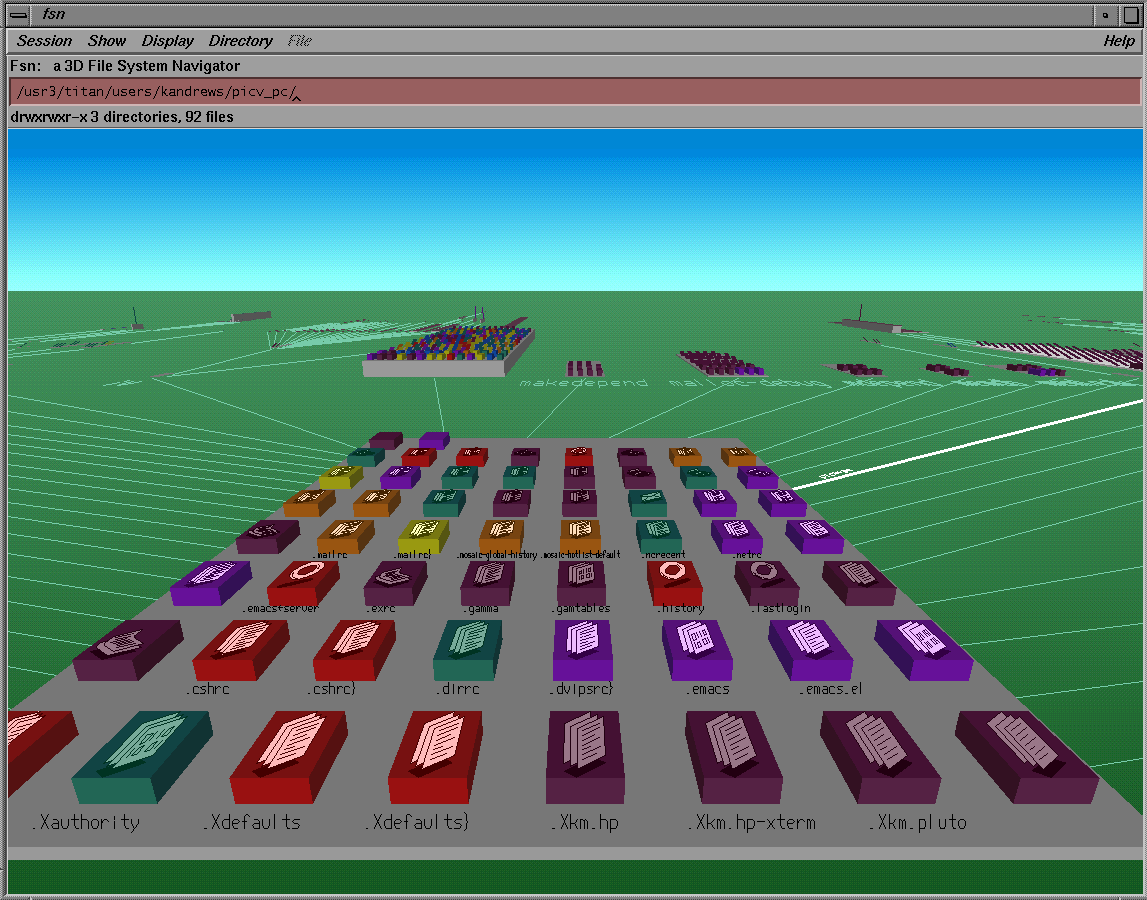
\includegraphics[width=8cm]{../grafik/fsn1.png}
\caption{FSN.}
\label{fig:fsn}
\end{figure}
\end{center}

\begin{center}
\begin{figure}[H]
    \centering
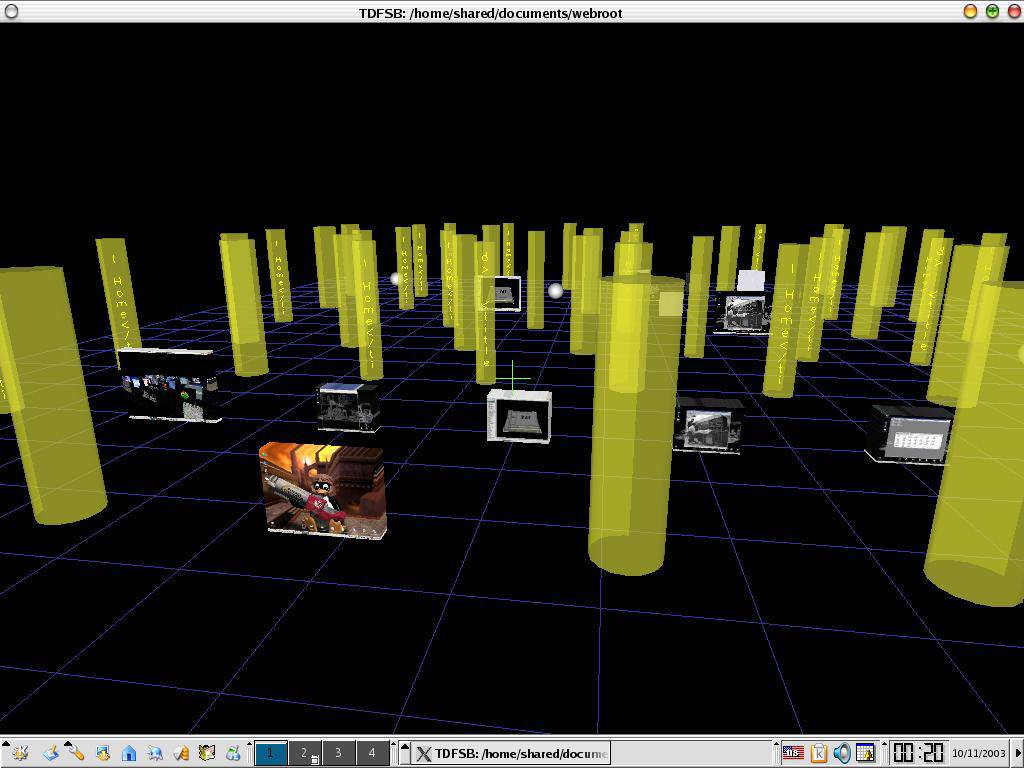
\includegraphics[width=8cm]{../grafik/tdfsb.jpg}
\caption{TDFSB.}
\label{fig:tdfsb}
\end{figure}
\end{center}

De ursprungliga obligatoriska kraven för produkten var följande:
\begin{LIPSkravlista}
\LIPSkrav{Original}{Alla filer ska representeras av block med någon textur på, är det en bild så ska bilden användas som textur}{1}

\LIPSkrav{Original}{Alla mappar ska representeras av block med någon textur}{1}
\LIPSkrav{Original}{Alla mappar och filer i en mapp ska vara placerade på en platta med en textur}{1}
\LIPSkrav{Original}{Ljussättningen ska ske med en Phong-shader}{1}
\LIPSkrav{Original}{Alla block ska ha skuggor}{1}
\LIPSkrav{Original}{Navigeringen ska vara first person där piltangenterna styr x och z koordinaterna och musen styr kameren i ett sfäriskt koordinatsystem}{1}
\LIPSkrav{Original}{Man ska inte kunna gå igenom filerna(collisions detection)}{1}
\LIPSkrav{Original}{Du ska kunna gå in i en mapp så transporteras du till den nya mappen)}{1}
\LIPSkrav{Original}{Du ska kunna klicka på en fil/mapp och få upp alla möjliga alternativ såsom radera, öppna...)}{1}
\LIPSkrav{Original}{Om du raderar en fil ska övriga filer ordna sig så det inte är några luckor någonstans}{1}
\LIPSkrav{Original}{Skydome ska finnas}{1}
\LIPSkrav{Original}{Endast Linux kommer stödjas}{1}
\end{LIPSkravlista}


och de ej obligatoriska kraven var följande:
\begin{LIPSkravlista}
\LIPSkrav{Original}{Du ska kunna få upp en terminal i filhanteraren}{2}
\LIPSkrav{Original}{Du ska kunna klicka på en mapp och sedan få upp en portal som du kan se in i mappen genom}{2}
\LIPSkrav{Original}{När du raderar en fil ska den explodera}{2}
\LIPSkrav{Original}{Innehåller en mapp många filer/mappar ska frustum culling användas för att minimera beräkningar}{2}
\LIPSkrav{Original}{Mapparnas texturer ska vara den ikon filen som operativsystemet använder med transparens, då ska renderingsordningen och vara korrekt}{2}
\end{LIPSkravlista}
Under projektets gång gick de obligatoriska kraven igenom en modifikation på grund av att projektet tog längre tid än vad jag trodde samt att en del inte riktigt passade in. Krav 5 togs bort på grund av tidsbrist, krav 6 gjordes om så att användaren bara navigerade i XZ planet då detta passade mycket bättre samt en del förenklingar kunde göras. Krav 9 togs bort då en terminal ansågs vara mycket enklare att implementera så all modifikation av filsystemet görs via den. Inga av de ej obligatorska kraven uppfylldes på grund av tidsbrist. I figur~\ref{fig:tmbtrf} kan man se resultatet. 
\begin{center}
\begin{figure}[H]
    \centering
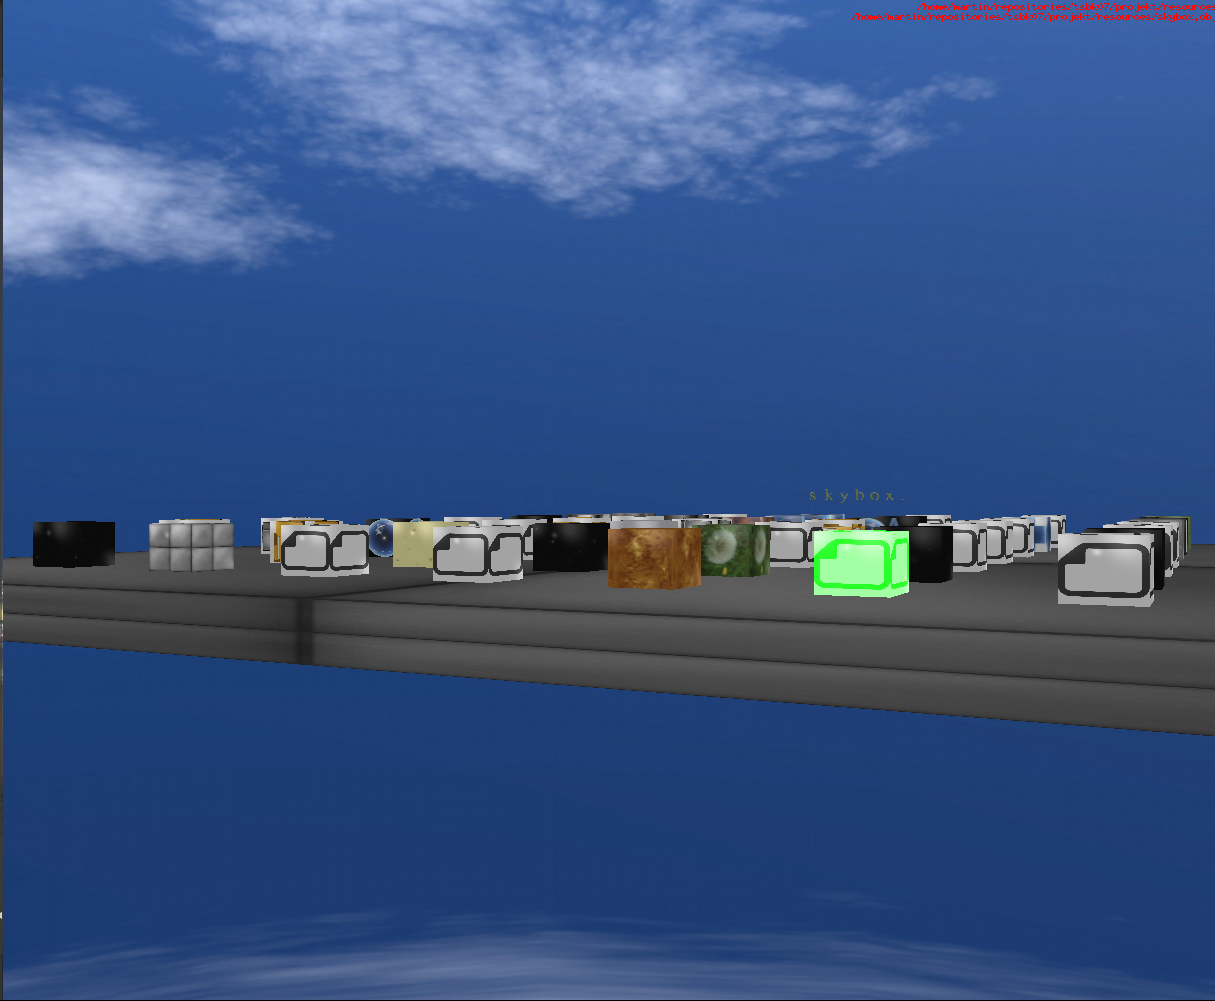
\includegraphics[width=8cm]{../grafik/tmbtrf.png}
\caption{TMBTRF.}
\label{fig:tmbtrf}
\end{figure}
\end{center}

\section{Bakgrund}
Det svåraste problemet jag hade innan jag började med projeketet var att på ett effektivt sätt interagera med datorns filsystem. Detta löstes rätt enkelt när jag upptäckte Boost::Filesystem. Detta bibliotek är inte speciellt använt så det finns inte så mycket hjälp att hitta på forum men dokumentation för det är väldigt bra så när jag väl kom in i det så fungera det väldigt bra. Funktioner såsom att byta namn och radera filer fanns redan implementerade så detta underlättade mycket.
\\
\\
Ett annat problem som var svårare än vad jag trodde var att visa filnamn i en 3D miljö. Den enklaste lösning skulle varit att använda något bibliotek för att generera texturer med en font till exempel FreeType. Jag försökte detta och jag kommer inte ihåg varför men jag fick det inte att fungera. För att få detta snyggt så skulle texturerna behöva vara transparenta så jag skulle behöva ta hänsynt till ordningen som alla objekt renderas. Min lösning på problemet var att generera .obj filer för alla tänkbara bokstäver och tecken som kan förekomma i ett filnamn. Jag valde alla bokstäver a-z och A-Z, alla siffror samt tecknen . - \_. Detta gjordes med ett python script i cad-programmet FreeCad. För att minimera inläsningstiden så läses alla dessa modeller in vid starten av programmet och återanvänds hela tiden. För att undvika problem som kan uppkomma vid långa filnamn som sträcker sig över hela miljön så visas bara de 7 första tecknen i filnamnet.
\\
\\
Anledningen till att C++ valdes var mest för dess datastrukturer såsom Vector, Map och string. Allting som kan göras i C++ kan självklart göras i C men där så är allting klart. Detta gjorde så att jag kunde göra en väldigt allmän klass som representerar alla objekt i 3D världen. Programmet arbetar också mycket med strängar och då är String väldigt mycket smidigare än en char array.
\\
\\
Ett problem som upptäcktes senare var att när man går in i en mapp som innehåller många filer, speciellt bilder, så tar det rätt lång tid innan hela världen har genererats. Detta skulle kunna lösas genom att ha en separat tråd som förbereder alla undermappar i den nuvarande mappen. Detta har dock inte implementeras men skulle jag fortsätta utveckla TMBTRF så skulle detta vara ett av de första problemen jag skulle lösa. 

\section{Teori}
I boken ''Software Product Quality Control'' \citep{SPQC} nämns ett antal definitioner som förtydligar vad kvalitetssäkring innebär, dessa syns nedan.  

\begin{itemize}
  \item ''Quality assurance: a planned and systematic pattern of all actions necessary to provide adequate confidence that an item or product conforms to established technical requirements.'' \citep[p.19]{SPQC} 
  \item ''Constructive quality assurance: All means to be used in constructing a product in a way so it meets its quality requirements.'' \citep[p.19]{SPQC} 
  \item ''Analyctical quality assurance: All means of analysing the state of the quality of a product.'' \citep[p.19]{SPQC} 
\end{itemize}
\noindent Kvalitetssäkring innebär följaktligen att man som leverantör av en produkt eller tjänst ska se till att de uppfyller de krav som har satts upp i en eventuell kravspecifikation. Det är dessa krav som sätter standarden för vad som är rätt nivå gällande kvalité. Under arbetsgången måste man analysera om man är på väg att uppfylla kraven eller inte, i sådana fall måste detta åtgärdas omedelbart.
\newline
\newline
Med detta sagt finns det flera steg i ett projekt att kvalitetssäkra. Ett effektivt sätt att göra detta på är genom att följa Shewhart cykeln, det vill säga planera, göra, studera och agera (PGSA) \citep{PDCA}. Shewhart cykeln är en iterativ fyra stegs metod, se figur \ref{fig:shewcycle}. Metoden är utvecklad av William Edwards Deming. Namnet ''Shewhart'' kommer från en av Demings kollegor \citep[p.~88]{Deming}. 
\begin{figure}[h]
\centerline{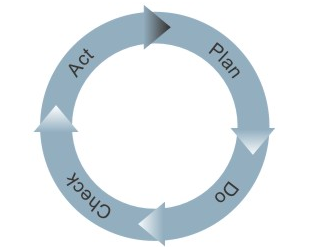
\includegraphics[scale=0.5]{ruben-tex/graphic/shewhartcycle}}
\caption{Shewhart cykeln \citep{Mindtools}}
\label{fig:shewcycle}
\end{figure}
\begin{enumerate}
  \item Planera. I detta skede ska målet fastställas, det vill säga sätta upp de krav som behövs för att kunden skall bli nöjd. Genom att göra detta är det tydligt om vad som skall göras och en överenskommelse finns mellan kund och leverantör. 
  \item Göra. När man konstaterat vad som behöver göras för att kunden skall bli nöjd är det dags att implementera ett sätt att arbeta och fullfölja processen.
  \item Studera. Efter att ha följt processen under en viss period är det dags att utvärdera om processen man har följt kommer leda till att man uppfyller de målen man har fastställt i planeringsfasen.
  \item Agera. Om man under studeringsfasen upptäcker att processen man följer inte kommer leda till att man uppfyller de krav som kund och leverantör var överens om måste detta åtgärdas omedelbart genom att planera om arbetsprocessen eller i viss mån diskutera kraven med kunden. Om processen som följs kommer uppfylla de krav som har satts upp kan man fortsätta med iterationerna av Shewhart cykeln precis som innan.
\end{enumerate}
\begin{figure}[h]
\centerline{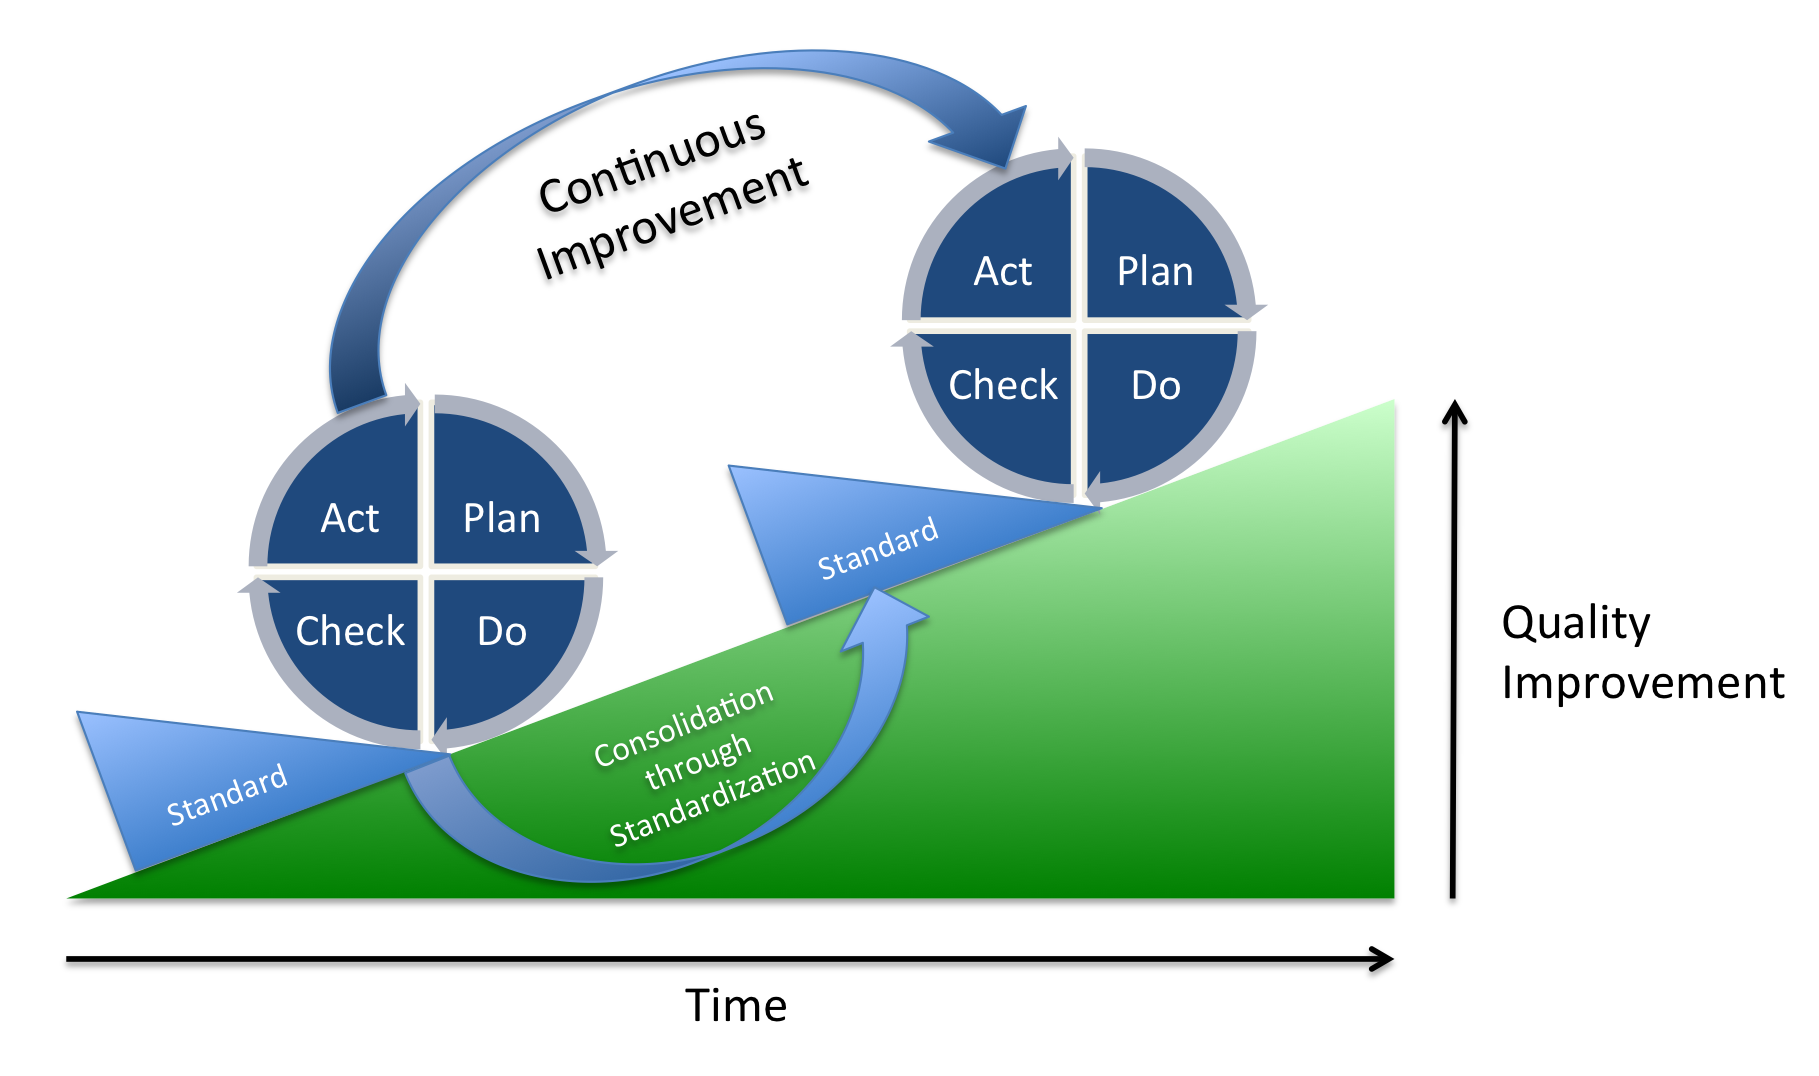
\includegraphics[scale=0.15]{ruben-tex/graphic/PDCA_Process}}
\caption{PDCA process \citep{Vietze}}
\label{fig:pdcaprocess}
\end{figure}
\noindent Genom att följa Shewhart cykeln under ett projekt kan man iterativt förbättra sin arbetsprocess och genom detta öka kvaliteten av den produkt man utvecklar, se figur \ref{fig:pdcaprocess}.
\newline
\newline
När det väl är dags för överlämning av en produkt eller tjänst är det bra att göra en kravinspektion innan. En kravinspektion enligt IEEE standarden för ''Software reviews'' syns nedan.

\begin{tcolorbox}[boxrule=1pt,leftrule=5pt,arc=0pt,auto outer arc]
\textbf{''}A process or meeting during which a software product is examined by a project personnel, managers, users, customers, user representatives, or other interested parties for comment or approval\textbf{''} \citep{SFSR}
\end{tcolorbox}

\noindent
Det man vill få gjort med en kravinspektion är alltså att produkten eller tjänsten som har tagits fram ska utvärderas av berörda parter så att den uppfyller de krav som har fastställts i ett tidigare skede för ett godkännande. En kravinspektion kan se ut som sådan \citep{Sandahl}:
\begin{enumerate}
\item{Tillträde.}
\item{Planering och översikt. Under detta steg sker en planering över hur inspektionen ska gå till och en översikt av produkten ges.}
\item{Individuell granskning. De berörda parterna granskar produkten eller tjänsten.}
\item{Möte. Efter granskningen görs en lista av alla de defekter som kan ha hittats.}
\item{Ändringar och uppföljning. I detta skede åtgärdar man de defekter som stöttes på och normalt brukar verifiera detta.}
\item{Utträde.}
\end{enumerate}

\subsection{Sammanfattning}
Sammanfattningsvis kan man konstatera att ett återkommande tema för att ta fram en högkvalitativ produkt eller tjänst är att planera, utföra och granska, för att sedan upprepa proceduren under projektets gång. Detta är dock bara en teoretisk tillämpning och verkligheten kan se annorlunda ut.

\section{Metod}
	För att ta reda på all information som behövs har ett flertal böcker blickats igenom. Ingen av dem har läst till 100\%, utan endast de intressanta delarna har läst med mer nogrannhet. För att verifiera att det som lästs stämmer har vissa delar testats i praktiken, i detta fall på projketet. Till exempel så har enhetstester körts på matris bibliotekts funktioner såsom matrisaddition, sytemtester och modultester har körts på den kvadratiska problem-lösaren och acceptanstester har körts på alla delar i projektet för att se till att alla krav är uppfyllda. Mer om detta kan läsas i resultat.
	
\subsection{Enhetstest}
	I ''Software Unit Testing'' \citep{ivv} definierar ett enhetstest som ett test på den minsta möjliga samlingen kod som fortfarande går att testa nyttofullt, alltså att koden är tillräckligt stor för att fel ska kunna uppstå. Dessa test är bra då de är riktade mot en så liten portion med kod och i och med detta sällan missar buggar och fel. Det som kan vara krångligt med enhetstest är att just hitta dessa minsta samlingarna med kod, speciellt om det är en extern part (en annan programmerare) som ska skapa och utföra testen. I och med att man kör enhetstester på så små delar av kod har de i teorin en tendens till att bli väldigt många om man ska täcka tillräckligt stor funktionalitet. Detta är dock oftast inget problem i praktiken eftersom många små funktioner ofta är triviala och har ytterst få uppgifter. Då behöver inte så många test skrivas, om ens ett enda.
\subsection{Modultest}	
	Det finns flera olika definitioner av vad en modul är, och i och med det blir det då svårt att definiera vad ett modultest är. I ''The Art of Software Testing'' definierar de att moduler och enheter är samma sak men jag har valt att istället gå efter Kristian Sandahls definiton. Han definierar att ett modultest är ett integrationtest utav två eller fler enheter. Det går ut på att man kombinerar ett antal enheter och sedan testar dem tillsammans. Testen i sig kan var väldigt lika enhetstest men täcker nu en mer komplex funktionalitet. Precis som enheter kan moduler vara svåra att definiera. Om allt för många enheter förs samman och modulen får mer funktionalitet kanske den till slut kan klassas som ett system, och då förlorar modultestningen sitt syfte. Om man har ett så litet projekt som detta så är moduldefinitionen ofta inte så svår, eftersom både komplexiteten och utvecklingsmöjligheterna är begränsade. Det är kritiskt vid dessa test att underliggande funktioner redan är testade. Om inte, kan i stort sett inga slutsatser, angående vad som är fel, dras när ett test misslyckas.
\subsection{Systemtest}	
	Ett systemtest är precis som modultest ett integrationstest, men nu utav ett antal moduler istället. Enligt ''The Art of Software Testing'' inriktar sig testet nu också vanligtvis på hela produkten som har utvecklats, för att se om funktionalitetskraven är uppfyllda. Detta för att säkerställa dess funktionalitet och för att hitta fel som uppstått vid kommunikation mellan moduler. Exempel på systemtest i vårt projekt är test av lösaren. Anledningen till att lösaren ses som ett eget system och inte är ihopbakad med GUI:t är att den ska kunna fungera separat. Givetvis är de båda ihopbakade också ett system, som också kräver systemtest.	
\subsection{Acceptanstest}	
	Ett acceptanstest är ett test som har målet att testa om programmet är acceptabelt. Med det menas att testen validerar ifall programmet uppfyller alla krav som ställs på det, och nu inte endast funktionalitetskraven. I vårt projekt är det huvudsakligen prestandan som behöver acceptanstestas. Då det prestandakrav produkten hade var relativt vagt ("Produkten ska ha likvärdig prestanda med Gurobi"), och att kravet sedan förhandlades bort, gjorde att testen inte hade så stor prioritet. Men för att få någon vetskap om produktens hastighet och för att garantera att kunden blir nöjd krävs ändå någon form utav test.
\subsection{Övrigt}	
	I projektet har även ett byggsystem använts, som smidigt kompilerat all kod automatiskt. Systemet har därefter även kört alla tester som skapats genom projektet.
	Med hjälp av byggsystemet och Kontinuerlig Integration har all kod då kunnat testas direkt när någon har skrivit ny kod och därav har det gått att se när och var feluppstått. Och eftersom systemet även har kört alla gamla test har koden säkerställts med att alla andra funktioner, de som inte har rörts, också fortfarande fungerar.
\section{Resultat}	
	Följande del beskriver hur arbetet med efterforskningen gick samt hur testen utfördes.
	\subsection{Efterforskning}
	Det finns otroligt mycket information om mjukvarutestning men samtidigt är ämnet ganska vagt då testning beror så mycket på just vad som ska testas. I vårt projekt visade det sig att ''Black Box''-testning var den metod som överlägset lämpade sig bäst. ''Black Box'' går ut på att man sätter en ''svart låda'' över det som ska testas, så att man endast kan se in- och utdatan. Sedan tittar man på utdata och ser ifall den är den förväntade. ''Black Box'' anses bra i detta projekt eftersom hela Quadopt är uppbyggd utav många små funktioner och resultateten som de ska ge tillbaka är oftast kända på förhand. Ett exempel på detta är matrisaritmetiken där resultatet, av till exempel en multiplikation, går att räkna ut ganska enkelt på papper. Enligt ''The Art of Software Testing'' ska dessa test utgå ifrån kravspecifikationen och andra dokument som beskriver vad produkten ska ha för funktionalitet. Boken beskriver också ''Black Box'' som en utmattande testteknik. Med det menar de att man borde testa alla möjliga indata till den svarta lådan och se så att svaren stämmer. Detta är precis som det står i boken i praktiken omöjligt. Speciellt i vårt projekt där det enda som begränsar antalet olika sätt en matris, bestående utav tal, kan se ut på är datorns minne. \newline
I projektet fanns dock ofta behovet av se en funktions lösningsgång, och då är ''Black Box'' en väldigt dålig metod. En metod som då lämpar sig bättre är ''White Box'' testning, som innebär att man tittar på den interna strukturen i en funktion. Därefter kan man se, efter vald indata, om lösningsgången är den väntade. I ''The Art of Software Testing'' står det att även denna metod kan problematisk då antalet lösningsgångar kan vara väldigt många. För att se om det ens är rimligt att utföra dessa test kan man se på funktionens cyklomatiska komplexitet. Cyklomatisk komplexitet innebär att man gör en graf över funktionen där de möjliga stadierna i lösningsgången är noder, och de möjliga lösningsvägarna är bågar. I ''Structured testing'' \citep{structest} står det att om denna komplexitet är för stor ökar antalet fel som programmeraren gjort väldigt fort, och samtidigt blir det i stort sett omöjligt att utföra några ''White Box''-test då fel kan uppstå på så många ställen. \\ 	
För att säkerställa projektets krav behövdes bara en testmetod till, och det var en metod för att mäta prestanda. Den som valdes var ''Load testing'' som innebär att man belastar programmet med mycket data och ser hur bra det fungerar. I projektets fall gavs lösaren många problem och tittade på hur fort det gick i förhållande till andra lösare. \newline	
Det skulle kunnat varit så att GUI:t hade haft högre prioritet än vad det hade. I det fallet hade olika typer av UX- och användartest varit nödvändiga för att kvalitetssäkra produkten. Men eftersom GUI:t beställdes utifrån kundens personliga behov, var det tydligt definierat redan från början att det var av låg prioritet. 
	
	\subsection{Praktik}
	Som beskrivet tidigare finns det i stort sett oändligt många kombinationer av in- och utdata.	För att då kunna utföra ''Black Box''-testerna behövdes antalet testfall reduceras. Detta åstadkoms genom att ha möten med kunden som klargjorde att indata till programmet alltid skulle vara giltig. Det reducerade antal testfall enormt mycket, men som beskrivet i resultatet av efterforskningen finns det även väldigt mycket giltig indata. Exempelvis för matrisaritmetiken. Dessa test gick också att reducera genom att de flesta operationer är triviala och endast kräver numeriska test såsom nolldivision och flyttalsfel. Genom att även utnyttja ''White Box''-tekniken gick det att utforma olika ''Black Box''-test som tog olika vägar genom koden och på så sätt bara skapa ett test för varje väg. Denna teknik utnyttjades endast på mindre funktioner såsom moduler för att antalet olika fall skulle begränsas till något som var rimligt. \newline
	För lösaren gick det att applicera samma metod, eftersom dess funktionalitet bygger mycket på underliggande funktioner. Det som skilde sig gentemot småfunktionerna var att nu behandlades oftast rader eller kolumner i matriser istället för enskilda element. Detta ledde till att de flesta test kontrollerade på kanterna utav det tillåtna området. Alltså kunde ett test vara att försöka hämta ut en radvektor på rad -1 ur en matris, vilket skulle vara ogiltigt.\newline
Vid granskning av testresultat från Git, Travis (verktyg för Kontinuerlig integration) och gruppmedlemmar visade det sig att majoriteten fel av bestod utav två typer: ''Assertion''s som misslyckats och ''Segmentation fault''. En ''Assertion'' är ett test inuti koden som avbryter exekveringen om testet inte går bra. ''Segmentation fault'' är ett programmeringsfel som resulterat i en ogiltig läsning eller skrivning till minnet. Felen som uppstod var väldigt utspridda och olika. Det som de flesta hade gemensamt var dock att de låg på en låg nivå, alltså i bottenfunktionerna. \newline	
	För att testa algoritmens hastighet stötte gruppen på oväntade problem, lösarna var för snabba.	Då varje testkörning tog 0.00 sekunder för alla lösarna förutom MATLAB behövdes testen köras många gånger för att se en tydlig skillnad. Anledningen till att MATLAB är långsammare är för att den är oerhört generell men förmodligen inte gjorts med fokus på att vara snabb. Gurobi är snabb eftersom dess enda uppgift är att lösa sådana här problem och har arbetats på under lång tid. Vår algoritm är snabb eftersom den inte är generell, alltså bryr vi oss inte om vissa specialfall som vi aldrig kommer stöta på. \newline
	För att då testa deras prestanda fick lösarna lösa olika optimeringsproblem många gånger, ofta upp emot 1000 gånger, för att kunna skilja deras egentliga hastighet. Att köra testen på vår lösare och i MATLAB var enkelt då vi hade funktionalitet för att konvertera matriser från MATLABs definition till vår, och vice versa. Däremot så var det krångligare i gurobi eftersom tiden som var allokerad för utbildning av programmet var begränsad. Det tvingade gruppen till att mata in problemet på ekvationsform vilket gjorde att gruppmedlemmarna var tvungna att köra endast små tester. Redan vid problem med fler än 10 bivillkor skulle det ta väldigt lång tid att konvertera och mata in problemet. \newline
	
	
	\subsection{Enhetstester}
	Under projektet har många enhetstest skrivits (framförallt för matrisbiblioteket). Dessa test har skrivits innan och under kodningen och sedan utförts direkt efter att koden blivit klar. Det som var intressant med dessa test var mängden av fel som upptäcktes direkt. Det ledde till att utvecklingen blev mycket effektiv då fel kunde åtgärdas direkt.
	
	\subsection{Integrationstester}
	De modultester som planerades och utfördes under projektet var framförallt lösarens funktioner. Modulerna var uppbyggda utav sammansättningar av enheter från matrisbiblioteket och andra strukturer. Dessa test utfördes vanligtvis samtidigt som implementeringen pågick. Detta för att hela tiden se till att rätt protokoll och gränssnitt användes.\\
De systemtester som utförts är tester utav lösaren och subproblemslösaren. Dessa ansågs vara tillräcklig komplexa för att ses som system. 
	
	
	\subsection{Acceptanstester}
	De acceptanstester som utförts under projektet är framförallt prestandatester. Detta då det enda kravet lösaren hade var att den skulle vara ungefär lika snabb som den kommersiella lösaren Gurobi. Då detta krav sedan togs bort lade mindre energi på prestandatester. Men de delar som ändå testats var framförallt underfunktioner till lösaren, såsom matrisbiblioteket och subproblemslösaren.
	
	\subsection{Misstag}
	Det hände att vissa modul- och systemtester skedde innan de underliggande enheterna blivit testade. Ett exempel på det är lösaren, som gruppen ivrigt ville få igång och började därför testa den tidigt. Då den inte fungerade korrekt gjorde detta att det tog lång tid att hitta felen som förmodligen hade upptäckts mycket snabbare om bara rätt testprocess hade använts.
	
	
\section{Diskussion}
Under denna del kommer en diskussion angående om resultaten ske samt metoderna som användes.
\subsection{Resultat}
Resultaten för alla tre punkter måste anses vara rimliga. Den första punkten angående vad som är rätt nivå är en väldigt diffus fråga och kan bara svaras genom att båda parter, dvs leverantör och kund har ett enhetligt svar. Eftersom det man kommer överens om i en eventuell kravspecifikation måste räcka att fullfölja för att det ska klassas som rätt nivå gällande kvalité. Sen om kunden hade velat haft några andra funktioner med produkten eller tjänsten så borde kunden ha specificerat detta. Leverantörer har också skyldighet att försöka uppfylla alla krav som har specificerats på ett snyggt sätt och inte bara slänga ihop något som fungerar, små detaljer kan utmärka ett arbete.
\newline
\newline
Den andra punkten finns det inte mycket att diskutera om, som allt annat i livet krävs det struktur för att man ska uppnå något. Under teoridelen i kapitel tre kan man konstatera att planera, utföra och granska antagligen kommer generera en produkt eller tjänst av tillräckligt god kvalité.
\newline
\newline
Angående den sista punkten kan man byta svaret från ett ja till ett nej, då ett krav förhandlades bort. I detta projekt hade kandidatgruppen endast ett mätbart krav, detta krav specificerade att optimeringsalgoritmen skulle vara likvärdig i hastighet i jämförelse med en kommersiell mjukvara kallad ''Gurobi''. ''Gurobi'' specialiserar sig i att lösa olika sorters optimeringsproblem \citep{gurobi}. Under projektets slutskede diskuterade kandidatgruppen med kunden om att det kommer bli svårt att vara jämbördig med ''Gurboi'', detta var inget problem för kunden och kravet kunde tas bort. Kunden tryckte på att det viktigaste var att koden fungerar och att den är väldokumenterad, vilket den är. Däremot kan jag tycka att om man tar bort ett krav så har man misslyckats och därför anser jag att man kan ändra svaret till nej, slutprodukten håller inte tillräckligt god kvalité, men då är jag väldigt hård mot mig själv och kandidatgruppen. Däremot säger teorin bakom det hela att produkten håller tillräckligt god nivå då den uppfyller alla krav, det ska inte spela någon roll om man har förhandlat bort något krav eller inte.

\subsection{Metod}
Efter slutförandet av projektet och analys av hur det hela gick finns det många saker man hade kunnat gjort annorlunda. Ett återkommande problem som stöttes på under projektets gång var att kodstandarden som hade satts upp från början inte följdes helt och hållet, inte förens den sista iterationen skrevs kod efter den. Detta resulterade i att mycket tid lades ner på att refaktorera kod. Kodstandarden innehöll inte heller allt som bör ta hänsyns till. Ett exempel är att frigöra minne, vilket resultera i att mycket tid lades ner på att hitta och åtgärda minnesläckor. Eftersom kandidatgruppen hade ett krav på att skriva pålitlig kod så är förstås minnesläckor inte accepterbart. 
\newline
\newline
Jag tror att slutprodukten skulle ha sett annorlunda ut om kodstandarden täckte fler områden i hur man ska skriva kod samt om man tryckte på hur viktigt det är att följa kodstandarden. Jag som kvalitetsamordnare hade kunnat trycka mer på att kodstandarden skall följas för att en produkt av bättre kvalité skulle skapats.
\newline
\newline
I teoridelen visade forskningen att om man ska uppnå en högkvalitativ produkt kan man t.ex. använda sig av Shewhart cykeln, planera, göra, studera och agera. Kandidatgruppen planera hur man skulle skriva kod, man följde inte kodstandarden, kandidatgruppen var väl medveten om det. Vid detta stadiet borde man agera, visserligen sas det åt folk att börja använda kodstandarden, men det hade nog varit bättre att utvärdera om kodstandarden och föra dialog om varför den inte följs för att skriva en ny som möjligtvis alla känner sig bekväma med.

\section{Slutsatser}
{\LaTeX} lämpar sig mycket väl för teknisk dokumentation i ett programmeringsprojekt. Denna slutsats kan dras från det {\LaTeX} dokument gruppen har producerat. {\LaTeX} gav oss verktygen för att infoga figurer, matematiska formler, ekvationer, algoritmer och pseudokod som behövdes för dokumenten i projektet.   
\newline
\newline
Det tog hela projekttiden för att samtliga medlemmar skulle känna att de behärskade {\LaTeX}. Detta kan ses som en lång inlärningskurva för språket och att det tog onödig tid från andra delar av projektet. Dock var detta aldrig egentligen något problem, mycket hjälp fanns att hämta från internet och då två av gruppmedlemmarna behärskade {\LaTeX} sedan tidigare kunde de hjälpa och lära resten av gruppen. 
\newline
\newline
Om ingen av gruppens medlemmar hade använt {\LaTeX} sedan tidigare kan det diskuteras om det hade varit lönsamt för gruppen att lära sig det. Då hade mer tid behövts läggas på utbildning av språket och andra uppgifter hade fått lida. Som sagt lämpar sig {\LaTeX} mycket väl för teknisk dokumentation i ett programmeringsprojekt och även om det hade tagit mer tid så hade det varit värt i det långa loppet.    
%Martins report
\stopcontents[sections]
\newpage

\resumecontents[default]
\addcontentsline{toc}{section}{\protect\numberline{C} Optimering av matrisbibliotek}
\stopcontents

\startcontents[sections]
\LIPSTitelsidamartin
\setcounter{section}{0} 
\printcontents[sections]{ }{1}{}
\newpage
\label{martins}
\section{Inledning}
Jag har gjort en filhanterar som visualiserar alla filer och mappar i 3D med hjälp av OpenGL. Inspirationen till detta projekt var bland annat FSN (File System Navigator) som gjordes av SGI för IRIX systemen och FSV(File System Visualizer) som är en remake av FSN på Linux, se figur~\ref{fig:fsn}. En annan inspiration var det lite modernare TDFSB som även visar upp bilder och filmer i 3D världen, se figur~\ref{fig:tdfsb}. 

\begin{center}
\begin{figure}[H]
    \centering
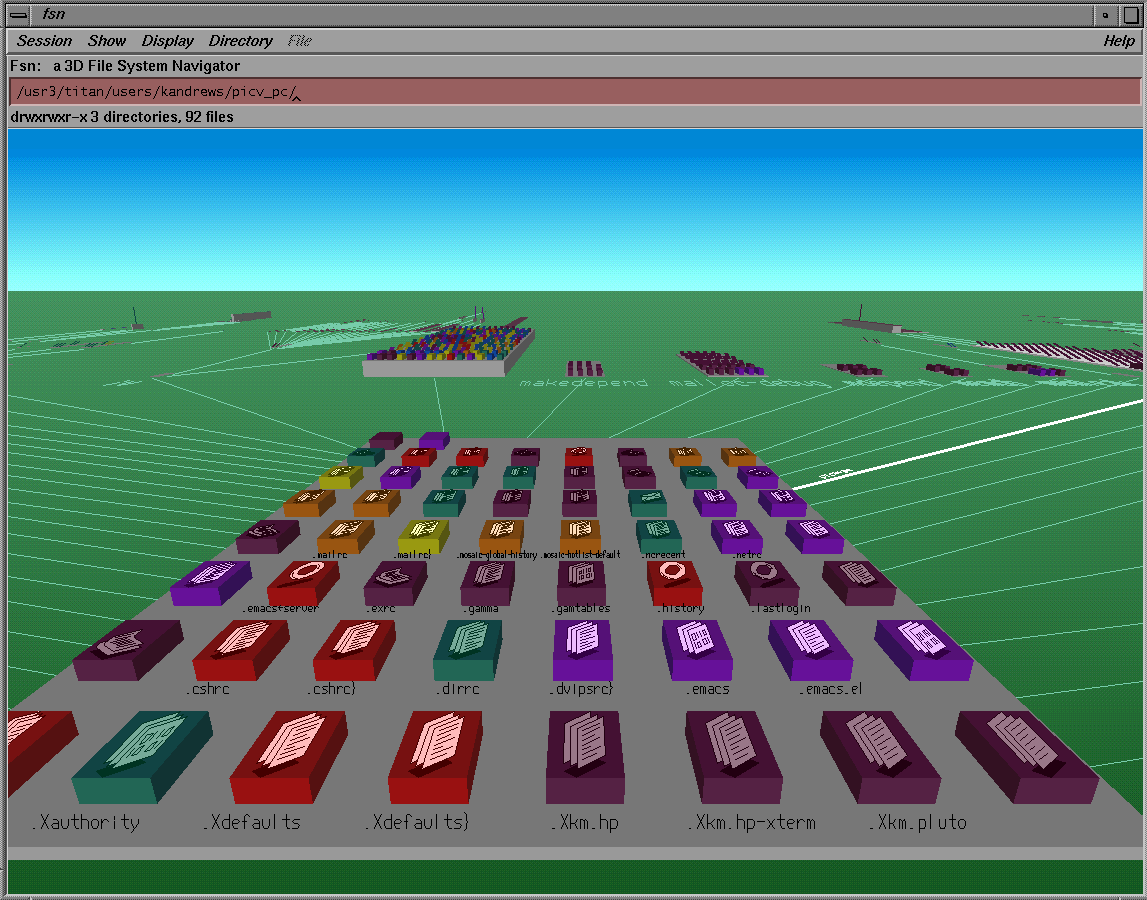
\includegraphics[width=8cm]{../grafik/fsn1.png}
\caption{FSN.}
\label{fig:fsn}
\end{figure}
\end{center}

\begin{center}
\begin{figure}[H]
    \centering
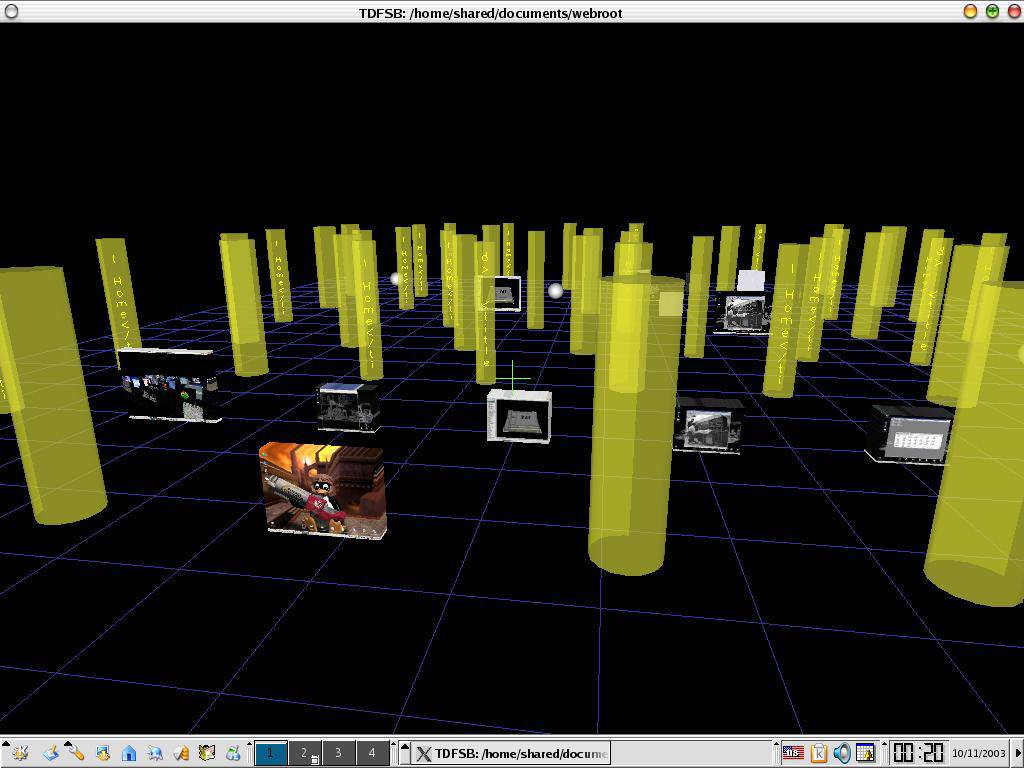
\includegraphics[width=8cm]{../grafik/tdfsb.jpg}
\caption{TDFSB.}
\label{fig:tdfsb}
\end{figure}
\end{center}

De ursprungliga obligatoriska kraven för produkten var följande:
\begin{LIPSkravlista}
\LIPSkrav{Original}{Alla filer ska representeras av block med någon textur på, är det en bild så ska bilden användas som textur}{1}

\LIPSkrav{Original}{Alla mappar ska representeras av block med någon textur}{1}
\LIPSkrav{Original}{Alla mappar och filer i en mapp ska vara placerade på en platta med en textur}{1}
\LIPSkrav{Original}{Ljussättningen ska ske med en Phong-shader}{1}
\LIPSkrav{Original}{Alla block ska ha skuggor}{1}
\LIPSkrav{Original}{Navigeringen ska vara first person där piltangenterna styr x och z koordinaterna och musen styr kameren i ett sfäriskt koordinatsystem}{1}
\LIPSkrav{Original}{Man ska inte kunna gå igenom filerna(collisions detection)}{1}
\LIPSkrav{Original}{Du ska kunna gå in i en mapp så transporteras du till den nya mappen)}{1}
\LIPSkrav{Original}{Du ska kunna klicka på en fil/mapp och få upp alla möjliga alternativ såsom radera, öppna...)}{1}
\LIPSkrav{Original}{Om du raderar en fil ska övriga filer ordna sig så det inte är några luckor någonstans}{1}
\LIPSkrav{Original}{Skydome ska finnas}{1}
\LIPSkrav{Original}{Endast Linux kommer stödjas}{1}
\end{LIPSkravlista}


och de ej obligatoriska kraven var följande:
\begin{LIPSkravlista}
\LIPSkrav{Original}{Du ska kunna få upp en terminal i filhanteraren}{2}
\LIPSkrav{Original}{Du ska kunna klicka på en mapp och sedan få upp en portal som du kan se in i mappen genom}{2}
\LIPSkrav{Original}{När du raderar en fil ska den explodera}{2}
\LIPSkrav{Original}{Innehåller en mapp många filer/mappar ska frustum culling användas för att minimera beräkningar}{2}
\LIPSkrav{Original}{Mapparnas texturer ska vara den ikon filen som operativsystemet använder med transparens, då ska renderingsordningen och vara korrekt}{2}
\end{LIPSkravlista}
Under projektets gång gick de obligatoriska kraven igenom en modifikation på grund av att projektet tog längre tid än vad jag trodde samt att en del inte riktigt passade in. Krav 5 togs bort på grund av tidsbrist, krav 6 gjordes om så att användaren bara navigerade i XZ planet då detta passade mycket bättre samt en del förenklingar kunde göras. Krav 9 togs bort då en terminal ansågs vara mycket enklare att implementera så all modifikation av filsystemet görs via den. Inga av de ej obligatorska kraven uppfylldes på grund av tidsbrist. I figur~\ref{fig:tmbtrf} kan man se resultatet. 
\begin{center}
\begin{figure}[H]
    \centering
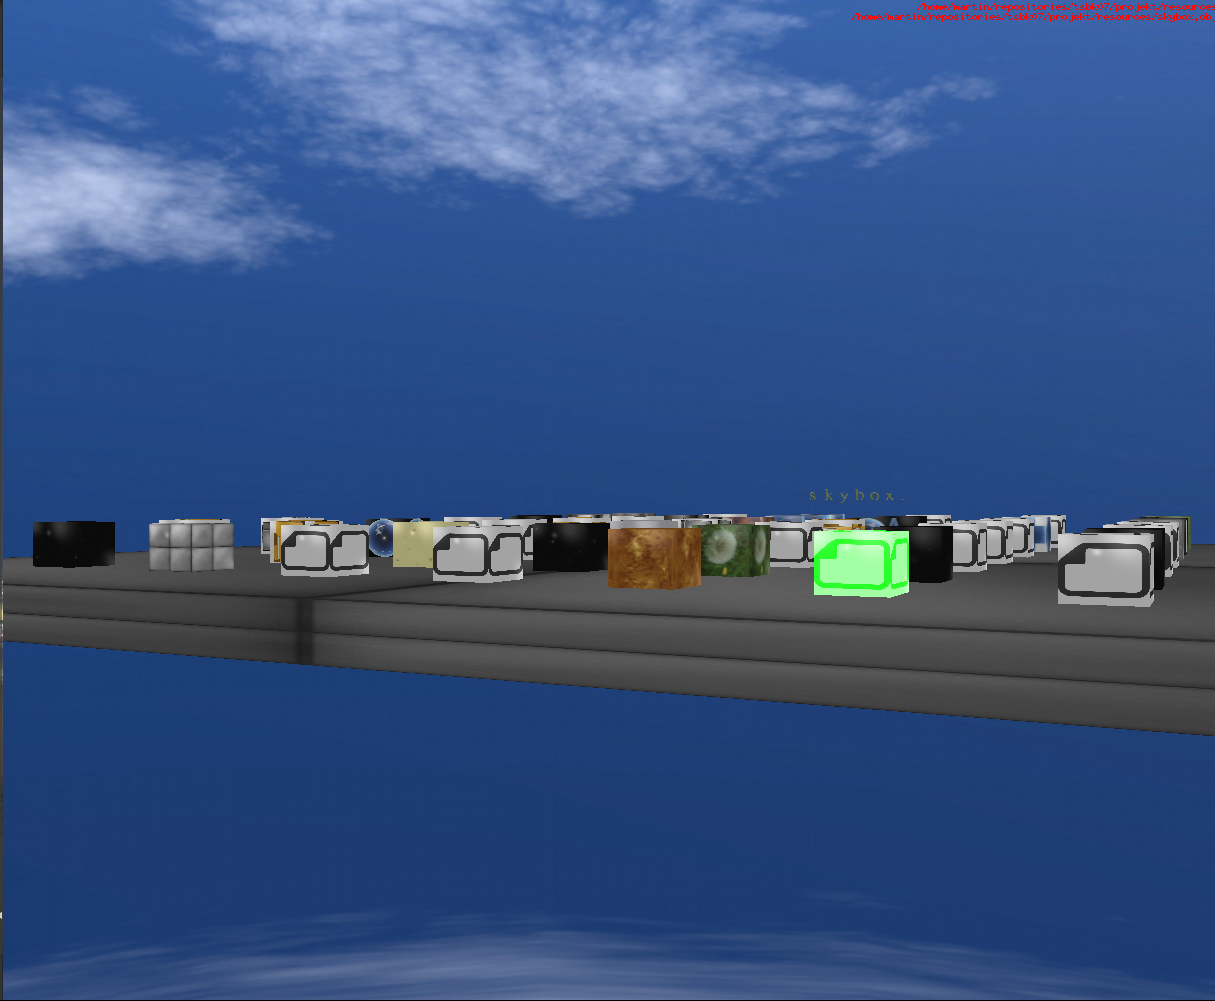
\includegraphics[width=8cm]{../grafik/tmbtrf.png}
\caption{TMBTRF.}
\label{fig:tmbtrf}
\end{figure}
\end{center}

\section{Bakgrund}
Det svåraste problemet jag hade innan jag började med projeketet var att på ett effektivt sätt interagera med datorns filsystem. Detta löstes rätt enkelt när jag upptäckte Boost::Filesystem. Detta bibliotek är inte speciellt använt så det finns inte så mycket hjälp att hitta på forum men dokumentation för det är väldigt bra så när jag väl kom in i det så fungera det väldigt bra. Funktioner såsom att byta namn och radera filer fanns redan implementerade så detta underlättade mycket.
\\
\\
Ett annat problem som var svårare än vad jag trodde var att visa filnamn i en 3D miljö. Den enklaste lösning skulle varit att använda något bibliotek för att generera texturer med en font till exempel FreeType. Jag försökte detta och jag kommer inte ihåg varför men jag fick det inte att fungera. För att få detta snyggt så skulle texturerna behöva vara transparenta så jag skulle behöva ta hänsynt till ordningen som alla objekt renderas. Min lösning på problemet var att generera .obj filer för alla tänkbara bokstäver och tecken som kan förekomma i ett filnamn. Jag valde alla bokstäver a-z och A-Z, alla siffror samt tecknen . - \_. Detta gjordes med ett python script i cad-programmet FreeCad. För att minimera inläsningstiden så läses alla dessa modeller in vid starten av programmet och återanvänds hela tiden. För att undvika problem som kan uppkomma vid långa filnamn som sträcker sig över hela miljön så visas bara de 7 första tecknen i filnamnet.
\\
\\
Anledningen till att C++ valdes var mest för dess datastrukturer såsom Vector, Map och string. Allting som kan göras i C++ kan självklart göras i C men där så är allting klart. Detta gjorde så att jag kunde göra en väldigt allmän klass som representerar alla objekt i 3D världen. Programmet arbetar också mycket med strängar och då är String väldigt mycket smidigare än en char array.
\\
\\
Ett problem som upptäcktes senare var att när man går in i en mapp som innehåller många filer, speciellt bilder, så tar det rätt lång tid innan hela världen har genererats. Detta skulle kunna lösas genom att ha en separat tråd som förbereder alla undermappar i den nuvarande mappen. Detta har dock inte implementeras men skulle jag fortsätta utveckla TMBTRF så skulle detta vara ett av de första problemen jag skulle lösa. 

\section{Teori}
I boken ''Software Product Quality Control'' \citep{SPQC} nämns ett antal definitioner som förtydligar vad kvalitetssäkring innebär, dessa syns nedan.  

\begin{itemize}
  \item ''Quality assurance: a planned and systematic pattern of all actions necessary to provide adequate confidence that an item or product conforms to established technical requirements.'' \citep[p.19]{SPQC} 
  \item ''Constructive quality assurance: All means to be used in constructing a product in a way so it meets its quality requirements.'' \citep[p.19]{SPQC} 
  \item ''Analyctical quality assurance: All means of analysing the state of the quality of a product.'' \citep[p.19]{SPQC} 
\end{itemize}
\noindent Kvalitetssäkring innebär följaktligen att man som leverantör av en produkt eller tjänst ska se till att de uppfyller de krav som har satts upp i en eventuell kravspecifikation. Det är dessa krav som sätter standarden för vad som är rätt nivå gällande kvalité. Under arbetsgången måste man analysera om man är på väg att uppfylla kraven eller inte, i sådana fall måste detta åtgärdas omedelbart.
\newline
\newline
Med detta sagt finns det flera steg i ett projekt att kvalitetssäkra. Ett effektivt sätt att göra detta på är genom att följa Shewhart cykeln, det vill säga planera, göra, studera och agera (PGSA) \citep{PDCA}. Shewhart cykeln är en iterativ fyra stegs metod, se figur \ref{fig:shewcycle}. Metoden är utvecklad av William Edwards Deming. Namnet ''Shewhart'' kommer från en av Demings kollegor \citep[p.~88]{Deming}. 
\begin{figure}[h]
\centerline{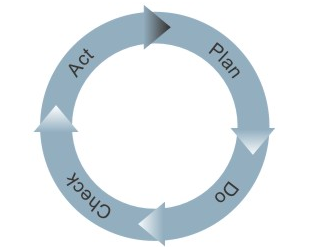
\includegraphics[scale=0.5]{ruben-tex/graphic/shewhartcycle}}
\caption{Shewhart cykeln \citep{Mindtools}}
\label{fig:shewcycle}
\end{figure}
\begin{enumerate}
  \item Planera. I detta skede ska målet fastställas, det vill säga sätta upp de krav som behövs för att kunden skall bli nöjd. Genom att göra detta är det tydligt om vad som skall göras och en överenskommelse finns mellan kund och leverantör. 
  \item Göra. När man konstaterat vad som behöver göras för att kunden skall bli nöjd är det dags att implementera ett sätt att arbeta och fullfölja processen.
  \item Studera. Efter att ha följt processen under en viss period är det dags att utvärdera om processen man har följt kommer leda till att man uppfyller de målen man har fastställt i planeringsfasen.
  \item Agera. Om man under studeringsfasen upptäcker att processen man följer inte kommer leda till att man uppfyller de krav som kund och leverantör var överens om måste detta åtgärdas omedelbart genom att planera om arbetsprocessen eller i viss mån diskutera kraven med kunden. Om processen som följs kommer uppfylla de krav som har satts upp kan man fortsätta med iterationerna av Shewhart cykeln precis som innan.
\end{enumerate}
\begin{figure}[h]
\centerline{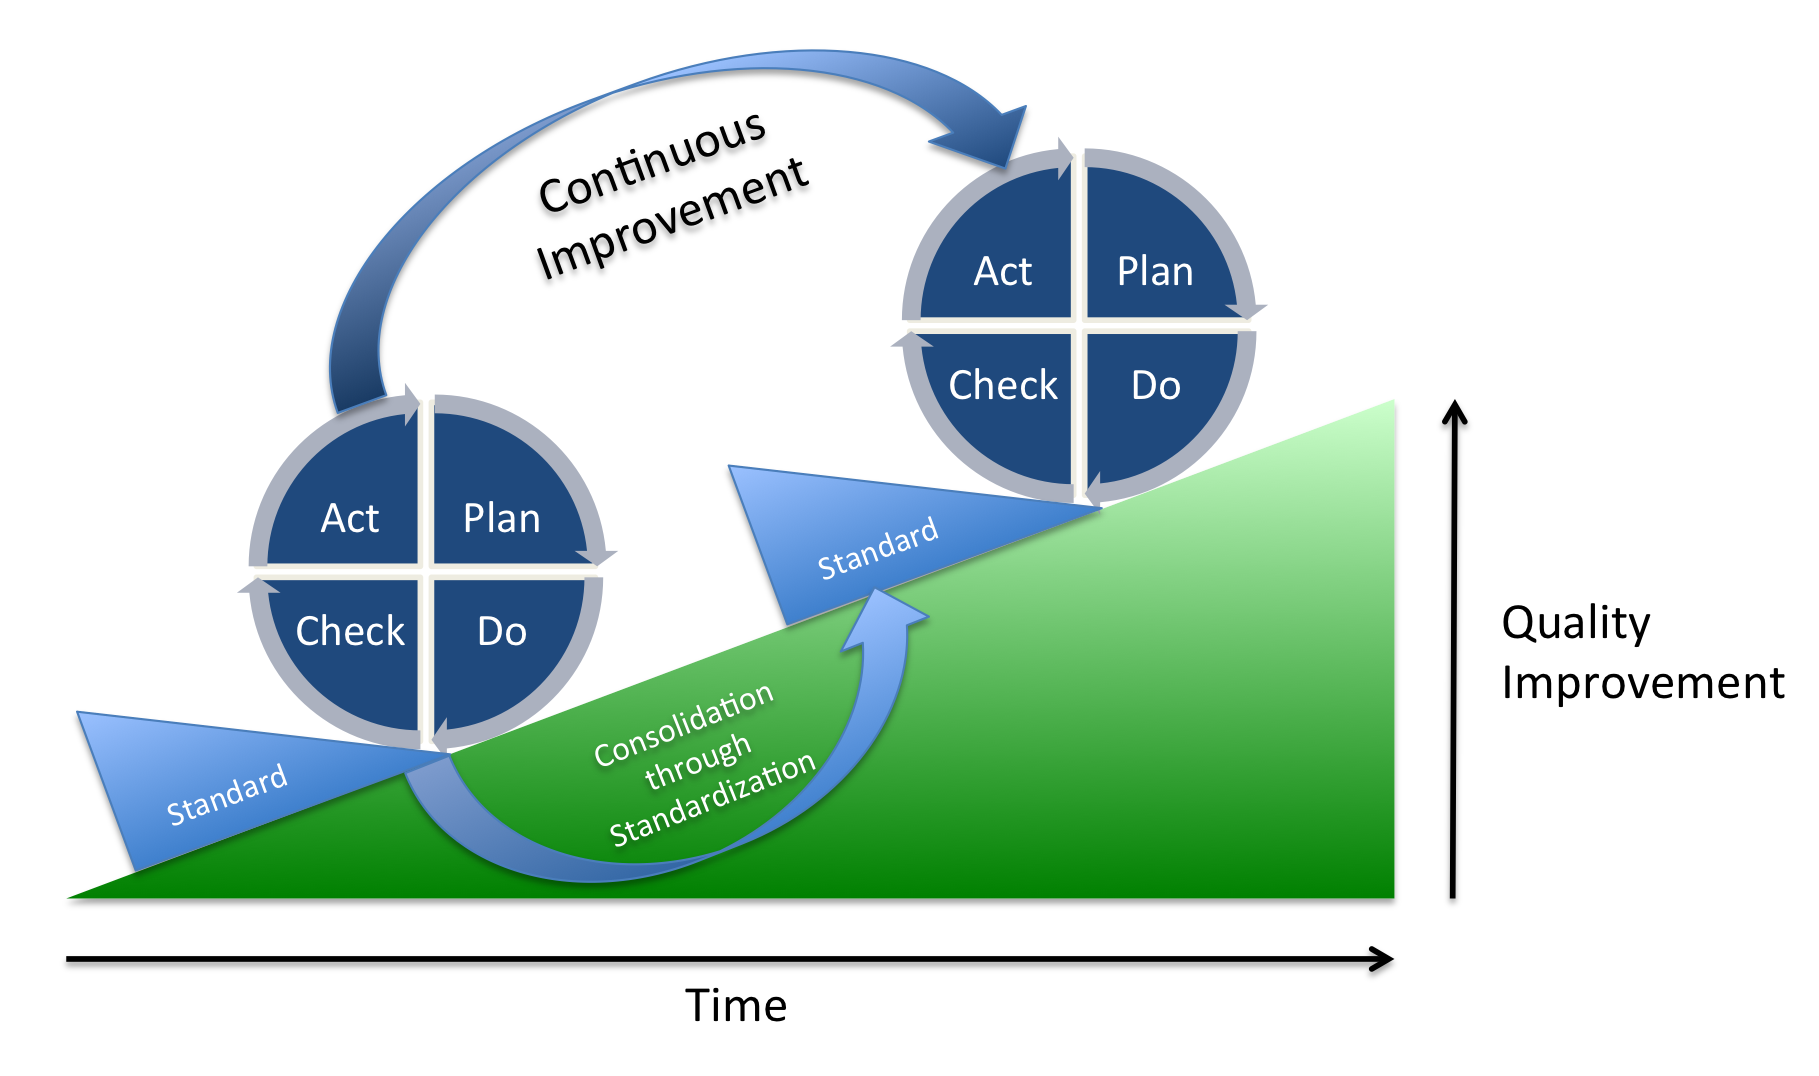
\includegraphics[scale=0.15]{ruben-tex/graphic/PDCA_Process}}
\caption{PDCA process \citep{Vietze}}
\label{fig:pdcaprocess}
\end{figure}
\noindent Genom att följa Shewhart cykeln under ett projekt kan man iterativt förbättra sin arbetsprocess och genom detta öka kvaliteten av den produkt man utvecklar, se figur \ref{fig:pdcaprocess}.
\newline
\newline
När det väl är dags för överlämning av en produkt eller tjänst är det bra att göra en kravinspektion innan. En kravinspektion enligt IEEE standarden för ''Software reviews'' syns nedan.

\begin{tcolorbox}[boxrule=1pt,leftrule=5pt,arc=0pt,auto outer arc]
\textbf{''}A process or meeting during which a software product is examined by a project personnel, managers, users, customers, user representatives, or other interested parties for comment or approval\textbf{''} \citep{SFSR}
\end{tcolorbox}

\noindent
Det man vill få gjort med en kravinspektion är alltså att produkten eller tjänsten som har tagits fram ska utvärderas av berörda parter så att den uppfyller de krav som har fastställts i ett tidigare skede för ett godkännande. En kravinspektion kan se ut som sådan \citep{Sandahl}:
\begin{enumerate}
\item{Tillträde.}
\item{Planering och översikt. Under detta steg sker en planering över hur inspektionen ska gå till och en översikt av produkten ges.}
\item{Individuell granskning. De berörda parterna granskar produkten eller tjänsten.}
\item{Möte. Efter granskningen görs en lista av alla de defekter som kan ha hittats.}
\item{Ändringar och uppföljning. I detta skede åtgärdar man de defekter som stöttes på och normalt brukar verifiera detta.}
\item{Utträde.}
\end{enumerate}

\subsection{Sammanfattning}
Sammanfattningsvis kan man konstatera att ett återkommande tema för att ta fram en högkvalitativ produkt eller tjänst är att planera, utföra och granska, för att sedan upprepa proceduren under projektets gång. Detta är dock bara en teoretisk tillämpning och verkligheten kan se annorlunda ut.

\section{Metod}
	För att ta reda på all information som behövs har ett flertal böcker blickats igenom. Ingen av dem har läst till 100\%, utan endast de intressanta delarna har läst med mer nogrannhet. För att verifiera att det som lästs stämmer har vissa delar testats i praktiken, i detta fall på projketet. Till exempel så har enhetstester körts på matris bibliotekts funktioner såsom matrisaddition, sytemtester och modultester har körts på den kvadratiska problem-lösaren och acceptanstester har körts på alla delar i projektet för att se till att alla krav är uppfyllda. Mer om detta kan läsas i resultat.
	
\subsection{Enhetstest}
	I ''Software Unit Testing'' \citep{ivv} definierar ett enhetstest som ett test på den minsta möjliga samlingen kod som fortfarande går att testa nyttofullt, alltså att koden är tillräckligt stor för att fel ska kunna uppstå. Dessa test är bra då de är riktade mot en så liten portion med kod och i och med detta sällan missar buggar och fel. Det som kan vara krångligt med enhetstest är att just hitta dessa minsta samlingarna med kod, speciellt om det är en extern part (en annan programmerare) som ska skapa och utföra testen. I och med att man kör enhetstester på så små delar av kod har de i teorin en tendens till att bli väldigt många om man ska täcka tillräckligt stor funktionalitet. Detta är dock oftast inget problem i praktiken eftersom många små funktioner ofta är triviala och har ytterst få uppgifter. Då behöver inte så många test skrivas, om ens ett enda.
\subsection{Modultest}	
	Det finns flera olika definitioner av vad en modul är, och i och med det blir det då svårt att definiera vad ett modultest är. I ''The Art of Software Testing'' definierar de att moduler och enheter är samma sak men jag har valt att istället gå efter Kristian Sandahls definiton. Han definierar att ett modultest är ett integrationtest utav två eller fler enheter. Det går ut på att man kombinerar ett antal enheter och sedan testar dem tillsammans. Testen i sig kan var väldigt lika enhetstest men täcker nu en mer komplex funktionalitet. Precis som enheter kan moduler vara svåra att definiera. Om allt för många enheter förs samman och modulen får mer funktionalitet kanske den till slut kan klassas som ett system, och då förlorar modultestningen sitt syfte. Om man har ett så litet projekt som detta så är moduldefinitionen ofta inte så svår, eftersom både komplexiteten och utvecklingsmöjligheterna är begränsade. Det är kritiskt vid dessa test att underliggande funktioner redan är testade. Om inte, kan i stort sett inga slutsatser, angående vad som är fel, dras när ett test misslyckas.
\subsection{Systemtest}	
	Ett systemtest är precis som modultest ett integrationstest, men nu utav ett antal moduler istället. Enligt ''The Art of Software Testing'' inriktar sig testet nu också vanligtvis på hela produkten som har utvecklats, för att se om funktionalitetskraven är uppfyllda. Detta för att säkerställa dess funktionalitet och för att hitta fel som uppstått vid kommunikation mellan moduler. Exempel på systemtest i vårt projekt är test av lösaren. Anledningen till att lösaren ses som ett eget system och inte är ihopbakad med GUI:t är att den ska kunna fungera separat. Givetvis är de båda ihopbakade också ett system, som också kräver systemtest.	
\subsection{Acceptanstest}	
	Ett acceptanstest är ett test som har målet att testa om programmet är acceptabelt. Med det menas att testen validerar ifall programmet uppfyller alla krav som ställs på det, och nu inte endast funktionalitetskraven. I vårt projekt är det huvudsakligen prestandan som behöver acceptanstestas. Då det prestandakrav produkten hade var relativt vagt ("Produkten ska ha likvärdig prestanda med Gurobi"), och att kravet sedan förhandlades bort, gjorde att testen inte hade så stor prioritet. Men för att få någon vetskap om produktens hastighet och för att garantera att kunden blir nöjd krävs ändå någon form utav test.
\subsection{Övrigt}	
	I projektet har även ett byggsystem använts, som smidigt kompilerat all kod automatiskt. Systemet har därefter även kört alla tester som skapats genom projektet.
	Med hjälp av byggsystemet och Kontinuerlig Integration har all kod då kunnat testas direkt när någon har skrivit ny kod och därav har det gått att se när och var feluppstått. Och eftersom systemet även har kört alla gamla test har koden säkerställts med att alla andra funktioner, de som inte har rörts, också fortfarande fungerar.
\section{Resultat}	
	Följande del beskriver hur arbetet med efterforskningen gick samt hur testen utfördes.
	\subsection{Efterforskning}
	Det finns otroligt mycket information om mjukvarutestning men samtidigt är ämnet ganska vagt då testning beror så mycket på just vad som ska testas. I vårt projekt visade det sig att ''Black Box''-testning var den metod som överlägset lämpade sig bäst. ''Black Box'' går ut på att man sätter en ''svart låda'' över det som ska testas, så att man endast kan se in- och utdatan. Sedan tittar man på utdata och ser ifall den är den förväntade. ''Black Box'' anses bra i detta projekt eftersom hela Quadopt är uppbyggd utav många små funktioner och resultateten som de ska ge tillbaka är oftast kända på förhand. Ett exempel på detta är matrisaritmetiken där resultatet, av till exempel en multiplikation, går att räkna ut ganska enkelt på papper. Enligt ''The Art of Software Testing'' ska dessa test utgå ifrån kravspecifikationen och andra dokument som beskriver vad produkten ska ha för funktionalitet. Boken beskriver också ''Black Box'' som en utmattande testteknik. Med det menar de att man borde testa alla möjliga indata till den svarta lådan och se så att svaren stämmer. Detta är precis som det står i boken i praktiken omöjligt. Speciellt i vårt projekt där det enda som begränsar antalet olika sätt en matris, bestående utav tal, kan se ut på är datorns minne. \newline
I projektet fanns dock ofta behovet av se en funktions lösningsgång, och då är ''Black Box'' en väldigt dålig metod. En metod som då lämpar sig bättre är ''White Box'' testning, som innebär att man tittar på den interna strukturen i en funktion. Därefter kan man se, efter vald indata, om lösningsgången är den väntade. I ''The Art of Software Testing'' står det att även denna metod kan problematisk då antalet lösningsgångar kan vara väldigt många. För att se om det ens är rimligt att utföra dessa test kan man se på funktionens cyklomatiska komplexitet. Cyklomatisk komplexitet innebär att man gör en graf över funktionen där de möjliga stadierna i lösningsgången är noder, och de möjliga lösningsvägarna är bågar. I ''Structured testing'' \citep{structest} står det att om denna komplexitet är för stor ökar antalet fel som programmeraren gjort väldigt fort, och samtidigt blir det i stort sett omöjligt att utföra några ''White Box''-test då fel kan uppstå på så många ställen. \\ 	
För att säkerställa projektets krav behövdes bara en testmetod till, och det var en metod för att mäta prestanda. Den som valdes var ''Load testing'' som innebär att man belastar programmet med mycket data och ser hur bra det fungerar. I projektets fall gavs lösaren många problem och tittade på hur fort det gick i förhållande till andra lösare. \newline	
Det skulle kunnat varit så att GUI:t hade haft högre prioritet än vad det hade. I det fallet hade olika typer av UX- och användartest varit nödvändiga för att kvalitetssäkra produkten. Men eftersom GUI:t beställdes utifrån kundens personliga behov, var det tydligt definierat redan från början att det var av låg prioritet. 
	
	\subsection{Praktik}
	Som beskrivet tidigare finns det i stort sett oändligt många kombinationer av in- och utdata.	För att då kunna utföra ''Black Box''-testerna behövdes antalet testfall reduceras. Detta åstadkoms genom att ha möten med kunden som klargjorde att indata till programmet alltid skulle vara giltig. Det reducerade antal testfall enormt mycket, men som beskrivet i resultatet av efterforskningen finns det även väldigt mycket giltig indata. Exempelvis för matrisaritmetiken. Dessa test gick också att reducera genom att de flesta operationer är triviala och endast kräver numeriska test såsom nolldivision och flyttalsfel. Genom att även utnyttja ''White Box''-tekniken gick det att utforma olika ''Black Box''-test som tog olika vägar genom koden och på så sätt bara skapa ett test för varje väg. Denna teknik utnyttjades endast på mindre funktioner såsom moduler för att antalet olika fall skulle begränsas till något som var rimligt. \newline
	För lösaren gick det att applicera samma metod, eftersom dess funktionalitet bygger mycket på underliggande funktioner. Det som skilde sig gentemot småfunktionerna var att nu behandlades oftast rader eller kolumner i matriser istället för enskilda element. Detta ledde till att de flesta test kontrollerade på kanterna utav det tillåtna området. Alltså kunde ett test vara att försöka hämta ut en radvektor på rad -1 ur en matris, vilket skulle vara ogiltigt.\newline
Vid granskning av testresultat från Git, Travis (verktyg för Kontinuerlig integration) och gruppmedlemmar visade det sig att majoriteten fel av bestod utav två typer: ''Assertion''s som misslyckats och ''Segmentation fault''. En ''Assertion'' är ett test inuti koden som avbryter exekveringen om testet inte går bra. ''Segmentation fault'' är ett programmeringsfel som resulterat i en ogiltig läsning eller skrivning till minnet. Felen som uppstod var väldigt utspridda och olika. Det som de flesta hade gemensamt var dock att de låg på en låg nivå, alltså i bottenfunktionerna. \newline	
	För att testa algoritmens hastighet stötte gruppen på oväntade problem, lösarna var för snabba.	Då varje testkörning tog 0.00 sekunder för alla lösarna förutom MATLAB behövdes testen köras många gånger för att se en tydlig skillnad. Anledningen till att MATLAB är långsammare är för att den är oerhört generell men förmodligen inte gjorts med fokus på att vara snabb. Gurobi är snabb eftersom dess enda uppgift är att lösa sådana här problem och har arbetats på under lång tid. Vår algoritm är snabb eftersom den inte är generell, alltså bryr vi oss inte om vissa specialfall som vi aldrig kommer stöta på. \newline
	För att då testa deras prestanda fick lösarna lösa olika optimeringsproblem många gånger, ofta upp emot 1000 gånger, för att kunna skilja deras egentliga hastighet. Att köra testen på vår lösare och i MATLAB var enkelt då vi hade funktionalitet för att konvertera matriser från MATLABs definition till vår, och vice versa. Däremot så var det krångligare i gurobi eftersom tiden som var allokerad för utbildning av programmet var begränsad. Det tvingade gruppen till att mata in problemet på ekvationsform vilket gjorde att gruppmedlemmarna var tvungna att köra endast små tester. Redan vid problem med fler än 10 bivillkor skulle det ta väldigt lång tid att konvertera och mata in problemet. \newline
	
	
	\subsection{Enhetstester}
	Under projektet har många enhetstest skrivits (framförallt för matrisbiblioteket). Dessa test har skrivits innan och under kodningen och sedan utförts direkt efter att koden blivit klar. Det som var intressant med dessa test var mängden av fel som upptäcktes direkt. Det ledde till att utvecklingen blev mycket effektiv då fel kunde åtgärdas direkt.
	
	\subsection{Integrationstester}
	De modultester som planerades och utfördes under projektet var framförallt lösarens funktioner. Modulerna var uppbyggda utav sammansättningar av enheter från matrisbiblioteket och andra strukturer. Dessa test utfördes vanligtvis samtidigt som implementeringen pågick. Detta för att hela tiden se till att rätt protokoll och gränssnitt användes.\\
De systemtester som utförts är tester utav lösaren och subproblemslösaren. Dessa ansågs vara tillräcklig komplexa för att ses som system. 
	
	
	\subsection{Acceptanstester}
	De acceptanstester som utförts under projektet är framförallt prestandatester. Detta då det enda kravet lösaren hade var att den skulle vara ungefär lika snabb som den kommersiella lösaren Gurobi. Då detta krav sedan togs bort lade mindre energi på prestandatester. Men de delar som ändå testats var framförallt underfunktioner till lösaren, såsom matrisbiblioteket och subproblemslösaren.
	
	\subsection{Misstag}
	Det hände att vissa modul- och systemtester skedde innan de underliggande enheterna blivit testade. Ett exempel på det är lösaren, som gruppen ivrigt ville få igång och började därför testa den tidigt. Då den inte fungerade korrekt gjorde detta att det tog lång tid att hitta felen som förmodligen hade upptäckts mycket snabbare om bara rätt testprocess hade använts.
	
	
\section{Diskussion}
Under denna del kommer en diskussion angående om resultaten ske samt metoderna som användes.
\subsection{Resultat}
Resultaten för alla tre punkter måste anses vara rimliga. Den första punkten angående vad som är rätt nivå är en väldigt diffus fråga och kan bara svaras genom att båda parter, dvs leverantör och kund har ett enhetligt svar. Eftersom det man kommer överens om i en eventuell kravspecifikation måste räcka att fullfölja för att det ska klassas som rätt nivå gällande kvalité. Sen om kunden hade velat haft några andra funktioner med produkten eller tjänsten så borde kunden ha specificerat detta. Leverantörer har också skyldighet att försöka uppfylla alla krav som har specificerats på ett snyggt sätt och inte bara slänga ihop något som fungerar, små detaljer kan utmärka ett arbete.
\newline
\newline
Den andra punkten finns det inte mycket att diskutera om, som allt annat i livet krävs det struktur för att man ska uppnå något. Under teoridelen i kapitel tre kan man konstatera att planera, utföra och granska antagligen kommer generera en produkt eller tjänst av tillräckligt god kvalité.
\newline
\newline
Angående den sista punkten kan man byta svaret från ett ja till ett nej, då ett krav förhandlades bort. I detta projekt hade kandidatgruppen endast ett mätbart krav, detta krav specificerade att optimeringsalgoritmen skulle vara likvärdig i hastighet i jämförelse med en kommersiell mjukvara kallad ''Gurobi''. ''Gurobi'' specialiserar sig i att lösa olika sorters optimeringsproblem \citep{gurobi}. Under projektets slutskede diskuterade kandidatgruppen med kunden om att det kommer bli svårt att vara jämbördig med ''Gurboi'', detta var inget problem för kunden och kravet kunde tas bort. Kunden tryckte på att det viktigaste var att koden fungerar och att den är väldokumenterad, vilket den är. Däremot kan jag tycka att om man tar bort ett krav så har man misslyckats och därför anser jag att man kan ändra svaret till nej, slutprodukten håller inte tillräckligt god kvalité, men då är jag väldigt hård mot mig själv och kandidatgruppen. Däremot säger teorin bakom det hela att produkten håller tillräckligt god nivå då den uppfyller alla krav, det ska inte spela någon roll om man har förhandlat bort något krav eller inte.

\subsection{Metod}
Efter slutförandet av projektet och analys av hur det hela gick finns det många saker man hade kunnat gjort annorlunda. Ett återkommande problem som stöttes på under projektets gång var att kodstandarden som hade satts upp från början inte följdes helt och hållet, inte förens den sista iterationen skrevs kod efter den. Detta resulterade i att mycket tid lades ner på att refaktorera kod. Kodstandarden innehöll inte heller allt som bör ta hänsyns till. Ett exempel är att frigöra minne, vilket resultera i att mycket tid lades ner på att hitta och åtgärda minnesläckor. Eftersom kandidatgruppen hade ett krav på att skriva pålitlig kod så är förstås minnesläckor inte accepterbart. 
\newline
\newline
Jag tror att slutprodukten skulle ha sett annorlunda ut om kodstandarden täckte fler områden i hur man ska skriva kod samt om man tryckte på hur viktigt det är att följa kodstandarden. Jag som kvalitetsamordnare hade kunnat trycka mer på att kodstandarden skall följas för att en produkt av bättre kvalité skulle skapats.
\newline
\newline
I teoridelen visade forskningen att om man ska uppnå en högkvalitativ produkt kan man t.ex. använda sig av Shewhart cykeln, planera, göra, studera och agera. Kandidatgruppen planera hur man skulle skriva kod, man följde inte kodstandarden, kandidatgruppen var väl medveten om det. Vid detta stadiet borde man agera, visserligen sas det åt folk att börja använda kodstandarden, men det hade nog varit bättre att utvärdera om kodstandarden och föra dialog om varför den inte följs för att skriva en ny som möjligtvis alla känner sig bekväma med.

\section{Slutsatser}
{\LaTeX} lämpar sig mycket väl för teknisk dokumentation i ett programmeringsprojekt. Denna slutsats kan dras från det {\LaTeX} dokument gruppen har producerat. {\LaTeX} gav oss verktygen för att infoga figurer, matematiska formler, ekvationer, algoritmer och pseudokod som behövdes för dokumenten i projektet.   
\newline
\newline
Det tog hela projekttiden för att samtliga medlemmar skulle känna att de behärskade {\LaTeX}. Detta kan ses som en lång inlärningskurva för språket och att det tog onödig tid från andra delar av projektet. Dock var detta aldrig egentligen något problem, mycket hjälp fanns att hämta från internet och då två av gruppmedlemmarna behärskade {\LaTeX} sedan tidigare kunde de hjälpa och lära resten av gruppen. 
\newline
\newline
Om ingen av gruppens medlemmar hade använt {\LaTeX} sedan tidigare kan det diskuteras om det hade varit lönsamt för gruppen att lära sig det. Då hade mer tid behövts läggas på utbildning av språket och andra uppgifter hade fått lida. Som sagt lämpar sig {\LaTeX} mycket väl för teknisk dokumentation i ett programmeringsprojekt och även om det hade tagit mer tid så hade det varit värt i det långa loppet.    
\stopcontents[sections]
\newpage

%Dennis report
\stopcontents
\resumecontents[default]
\addcontentsline{toc}{section}{\protect\numberline{D} \LaTeX \ för teknisk dokumentation}
\stopcontents
\startcontents[sections]
\LIPSTitelsidadennis
\setcounter{section}{0} 
\newpage
\printcontents[sections]{ }{1}{}
\newpage
\section{Inledning}
Jag har gjort en filhanterar som visualiserar alla filer och mappar i 3D med hjälp av OpenGL. Inspirationen till detta projekt var bland annat FSN (File System Navigator) som gjordes av SGI för IRIX systemen och FSV(File System Visualizer) som är en remake av FSN på Linux, se figur~\ref{fig:fsn}. En annan inspiration var det lite modernare TDFSB som även visar upp bilder och filmer i 3D världen, se figur~\ref{fig:tdfsb}. 

\begin{center}
\begin{figure}[H]
    \centering
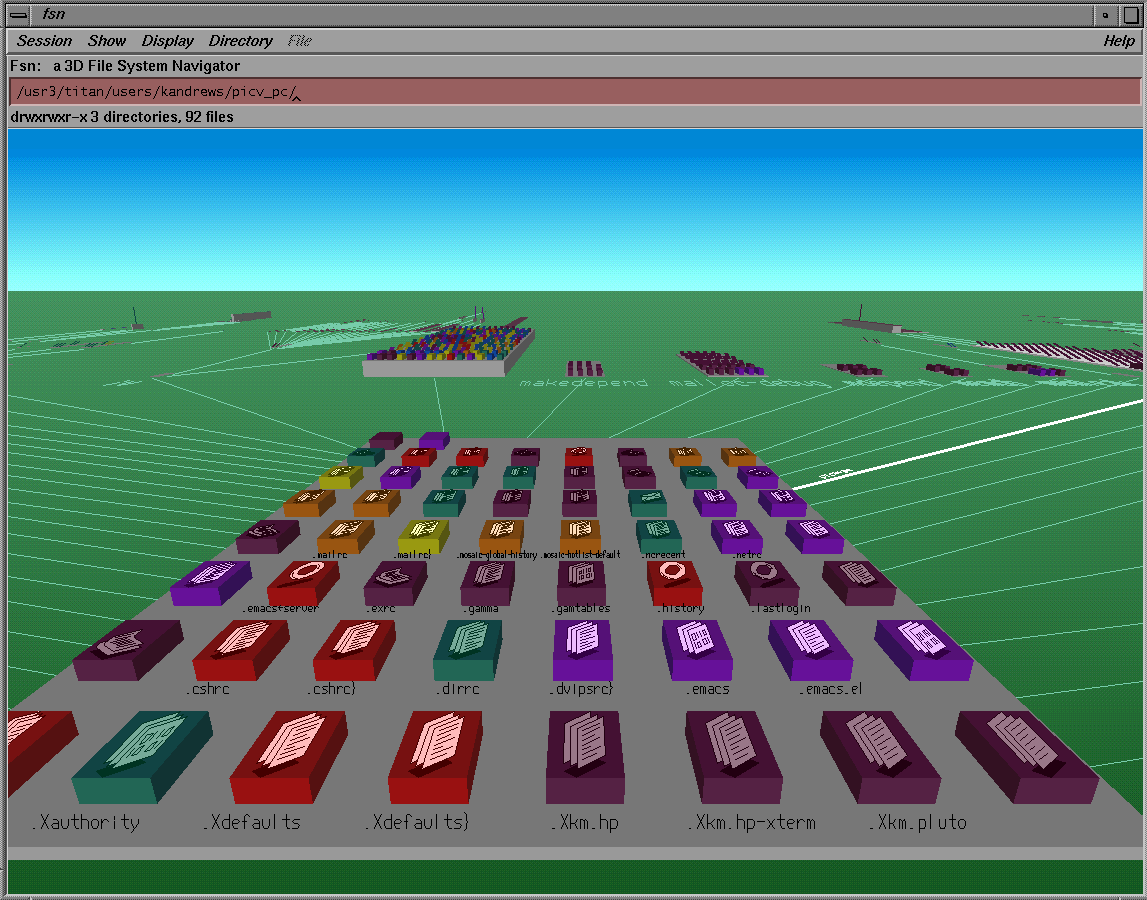
\includegraphics[width=8cm]{../grafik/fsn1.png}
\caption{FSN.}
\label{fig:fsn}
\end{figure}
\end{center}

\begin{center}
\begin{figure}[H]
    \centering
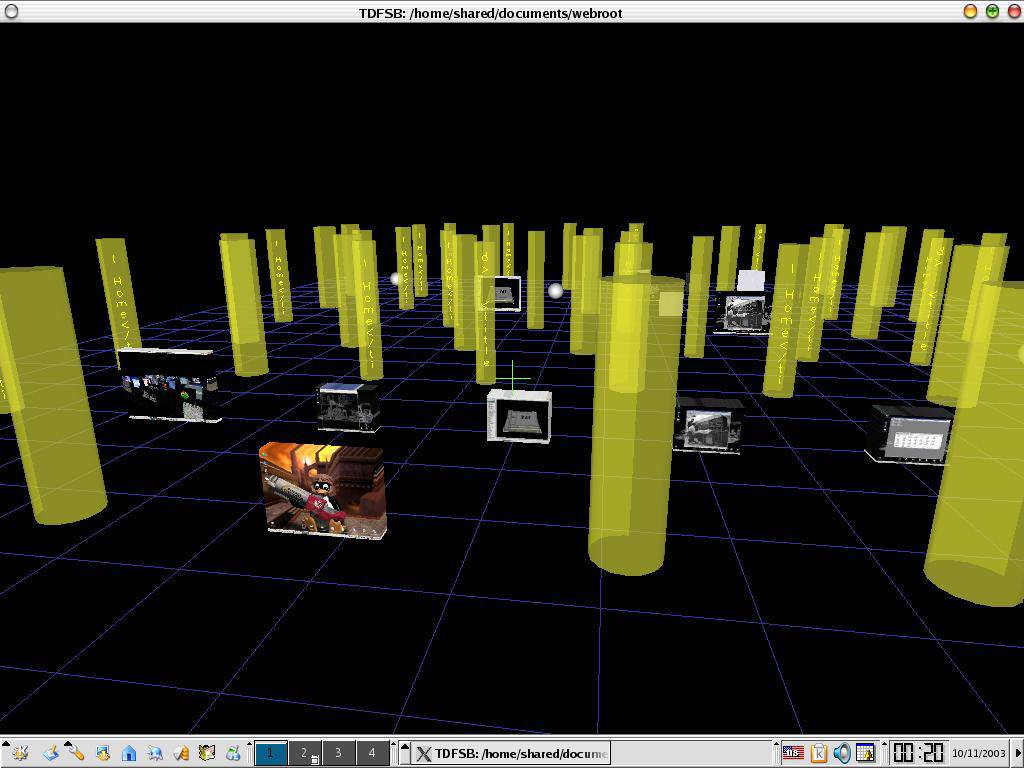
\includegraphics[width=8cm]{../grafik/tdfsb.jpg}
\caption{TDFSB.}
\label{fig:tdfsb}
\end{figure}
\end{center}

De ursprungliga obligatoriska kraven för produkten var följande:
\begin{LIPSkravlista}
\LIPSkrav{Original}{Alla filer ska representeras av block med någon textur på, är det en bild så ska bilden användas som textur}{1}

\LIPSkrav{Original}{Alla mappar ska representeras av block med någon textur}{1}
\LIPSkrav{Original}{Alla mappar och filer i en mapp ska vara placerade på en platta med en textur}{1}
\LIPSkrav{Original}{Ljussättningen ska ske med en Phong-shader}{1}
\LIPSkrav{Original}{Alla block ska ha skuggor}{1}
\LIPSkrav{Original}{Navigeringen ska vara first person där piltangenterna styr x och z koordinaterna och musen styr kameren i ett sfäriskt koordinatsystem}{1}
\LIPSkrav{Original}{Man ska inte kunna gå igenom filerna(collisions detection)}{1}
\LIPSkrav{Original}{Du ska kunna gå in i en mapp så transporteras du till den nya mappen)}{1}
\LIPSkrav{Original}{Du ska kunna klicka på en fil/mapp och få upp alla möjliga alternativ såsom radera, öppna...)}{1}
\LIPSkrav{Original}{Om du raderar en fil ska övriga filer ordna sig så det inte är några luckor någonstans}{1}
\LIPSkrav{Original}{Skydome ska finnas}{1}
\LIPSkrav{Original}{Endast Linux kommer stödjas}{1}
\end{LIPSkravlista}


och de ej obligatoriska kraven var följande:
\begin{LIPSkravlista}
\LIPSkrav{Original}{Du ska kunna få upp en terminal i filhanteraren}{2}
\LIPSkrav{Original}{Du ska kunna klicka på en mapp och sedan få upp en portal som du kan se in i mappen genom}{2}
\LIPSkrav{Original}{När du raderar en fil ska den explodera}{2}
\LIPSkrav{Original}{Innehåller en mapp många filer/mappar ska frustum culling användas för att minimera beräkningar}{2}
\LIPSkrav{Original}{Mapparnas texturer ska vara den ikon filen som operativsystemet använder med transparens, då ska renderingsordningen och vara korrekt}{2}
\end{LIPSkravlista}
Under projektets gång gick de obligatoriska kraven igenom en modifikation på grund av att projektet tog längre tid än vad jag trodde samt att en del inte riktigt passade in. Krav 5 togs bort på grund av tidsbrist, krav 6 gjordes om så att användaren bara navigerade i XZ planet då detta passade mycket bättre samt en del förenklingar kunde göras. Krav 9 togs bort då en terminal ansågs vara mycket enklare att implementera så all modifikation av filsystemet görs via den. Inga av de ej obligatorska kraven uppfylldes på grund av tidsbrist. I figur~\ref{fig:tmbtrf} kan man se resultatet. 
\begin{center}
\begin{figure}[H]
    \centering
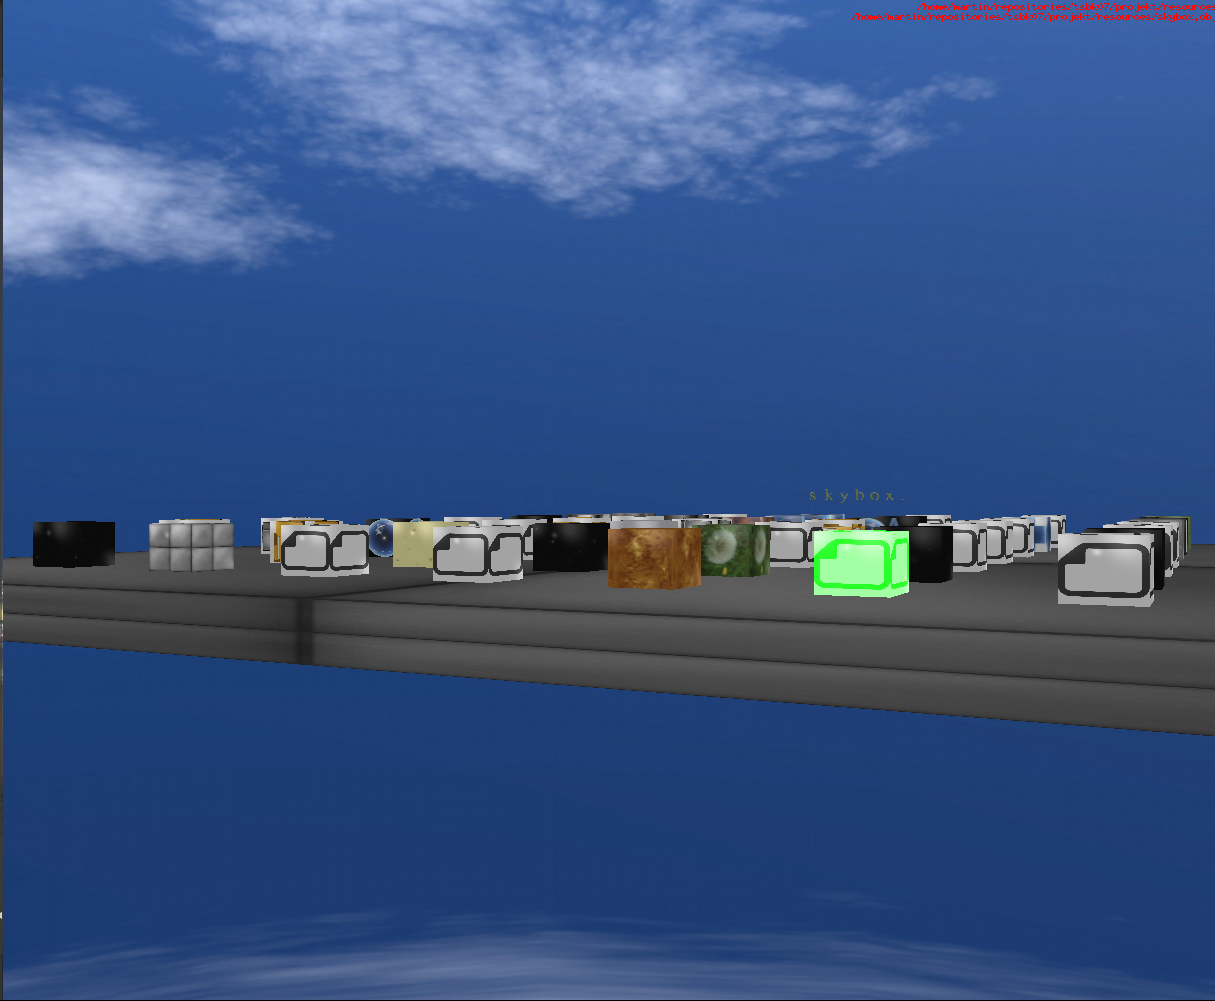
\includegraphics[width=8cm]{../grafik/tmbtrf.png}
\caption{TMBTRF.}
\label{fig:tmbtrf}
\end{figure}
\end{center}

\section{Bakgrund}
Det svåraste problemet jag hade innan jag började med projeketet var att på ett effektivt sätt interagera med datorns filsystem. Detta löstes rätt enkelt när jag upptäckte Boost::Filesystem. Detta bibliotek är inte speciellt använt så det finns inte så mycket hjälp att hitta på forum men dokumentation för det är väldigt bra så när jag väl kom in i det så fungera det väldigt bra. Funktioner såsom att byta namn och radera filer fanns redan implementerade så detta underlättade mycket.
\\
\\
Ett annat problem som var svårare än vad jag trodde var att visa filnamn i en 3D miljö. Den enklaste lösning skulle varit att använda något bibliotek för att generera texturer med en font till exempel FreeType. Jag försökte detta och jag kommer inte ihåg varför men jag fick det inte att fungera. För att få detta snyggt så skulle texturerna behöva vara transparenta så jag skulle behöva ta hänsynt till ordningen som alla objekt renderas. Min lösning på problemet var att generera .obj filer för alla tänkbara bokstäver och tecken som kan förekomma i ett filnamn. Jag valde alla bokstäver a-z och A-Z, alla siffror samt tecknen . - \_. Detta gjordes med ett python script i cad-programmet FreeCad. För att minimera inläsningstiden så läses alla dessa modeller in vid starten av programmet och återanvänds hela tiden. För att undvika problem som kan uppkomma vid långa filnamn som sträcker sig över hela miljön så visas bara de 7 första tecknen i filnamnet.
\\
\\
Anledningen till att C++ valdes var mest för dess datastrukturer såsom Vector, Map och string. Allting som kan göras i C++ kan självklart göras i C men där så är allting klart. Detta gjorde så att jag kunde göra en väldigt allmän klass som representerar alla objekt i 3D världen. Programmet arbetar också mycket med strängar och då är String väldigt mycket smidigare än en char array.
\\
\\
Ett problem som upptäcktes senare var att när man går in i en mapp som innehåller många filer, speciellt bilder, så tar det rätt lång tid innan hela världen har genererats. Detta skulle kunna lösas genom att ha en separat tråd som förbereder alla undermappar i den nuvarande mappen. Detta har dock inte implementeras men skulle jag fortsätta utveckla TMBTRF så skulle detta vara ett av de första problemen jag skulle lösa. 

\section{Teori}
I boken ''Software Product Quality Control'' \citep{SPQC} nämns ett antal definitioner som förtydligar vad kvalitetssäkring innebär, dessa syns nedan.  

\begin{itemize}
  \item ''Quality assurance: a planned and systematic pattern of all actions necessary to provide adequate confidence that an item or product conforms to established technical requirements.'' \citep[p.19]{SPQC} 
  \item ''Constructive quality assurance: All means to be used in constructing a product in a way so it meets its quality requirements.'' \citep[p.19]{SPQC} 
  \item ''Analyctical quality assurance: All means of analysing the state of the quality of a product.'' \citep[p.19]{SPQC} 
\end{itemize}
\noindent Kvalitetssäkring innebär följaktligen att man som leverantör av en produkt eller tjänst ska se till att de uppfyller de krav som har satts upp i en eventuell kravspecifikation. Det är dessa krav som sätter standarden för vad som är rätt nivå gällande kvalité. Under arbetsgången måste man analysera om man är på väg att uppfylla kraven eller inte, i sådana fall måste detta åtgärdas omedelbart.
\newline
\newline
Med detta sagt finns det flera steg i ett projekt att kvalitetssäkra. Ett effektivt sätt att göra detta på är genom att följa Shewhart cykeln, det vill säga planera, göra, studera och agera (PGSA) \citep{PDCA}. Shewhart cykeln är en iterativ fyra stegs metod, se figur \ref{fig:shewcycle}. Metoden är utvecklad av William Edwards Deming. Namnet ''Shewhart'' kommer från en av Demings kollegor \citep[p.~88]{Deming}. 
\begin{figure}[h]
\centerline{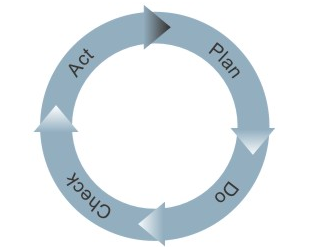
\includegraphics[scale=0.5]{ruben-tex/graphic/shewhartcycle}}
\caption{Shewhart cykeln \citep{Mindtools}}
\label{fig:shewcycle}
\end{figure}
\begin{enumerate}
  \item Planera. I detta skede ska målet fastställas, det vill säga sätta upp de krav som behövs för att kunden skall bli nöjd. Genom att göra detta är det tydligt om vad som skall göras och en överenskommelse finns mellan kund och leverantör. 
  \item Göra. När man konstaterat vad som behöver göras för att kunden skall bli nöjd är det dags att implementera ett sätt att arbeta och fullfölja processen.
  \item Studera. Efter att ha följt processen under en viss period är det dags att utvärdera om processen man har följt kommer leda till att man uppfyller de målen man har fastställt i planeringsfasen.
  \item Agera. Om man under studeringsfasen upptäcker att processen man följer inte kommer leda till att man uppfyller de krav som kund och leverantör var överens om måste detta åtgärdas omedelbart genom att planera om arbetsprocessen eller i viss mån diskutera kraven med kunden. Om processen som följs kommer uppfylla de krav som har satts upp kan man fortsätta med iterationerna av Shewhart cykeln precis som innan.
\end{enumerate}
\begin{figure}[h]
\centerline{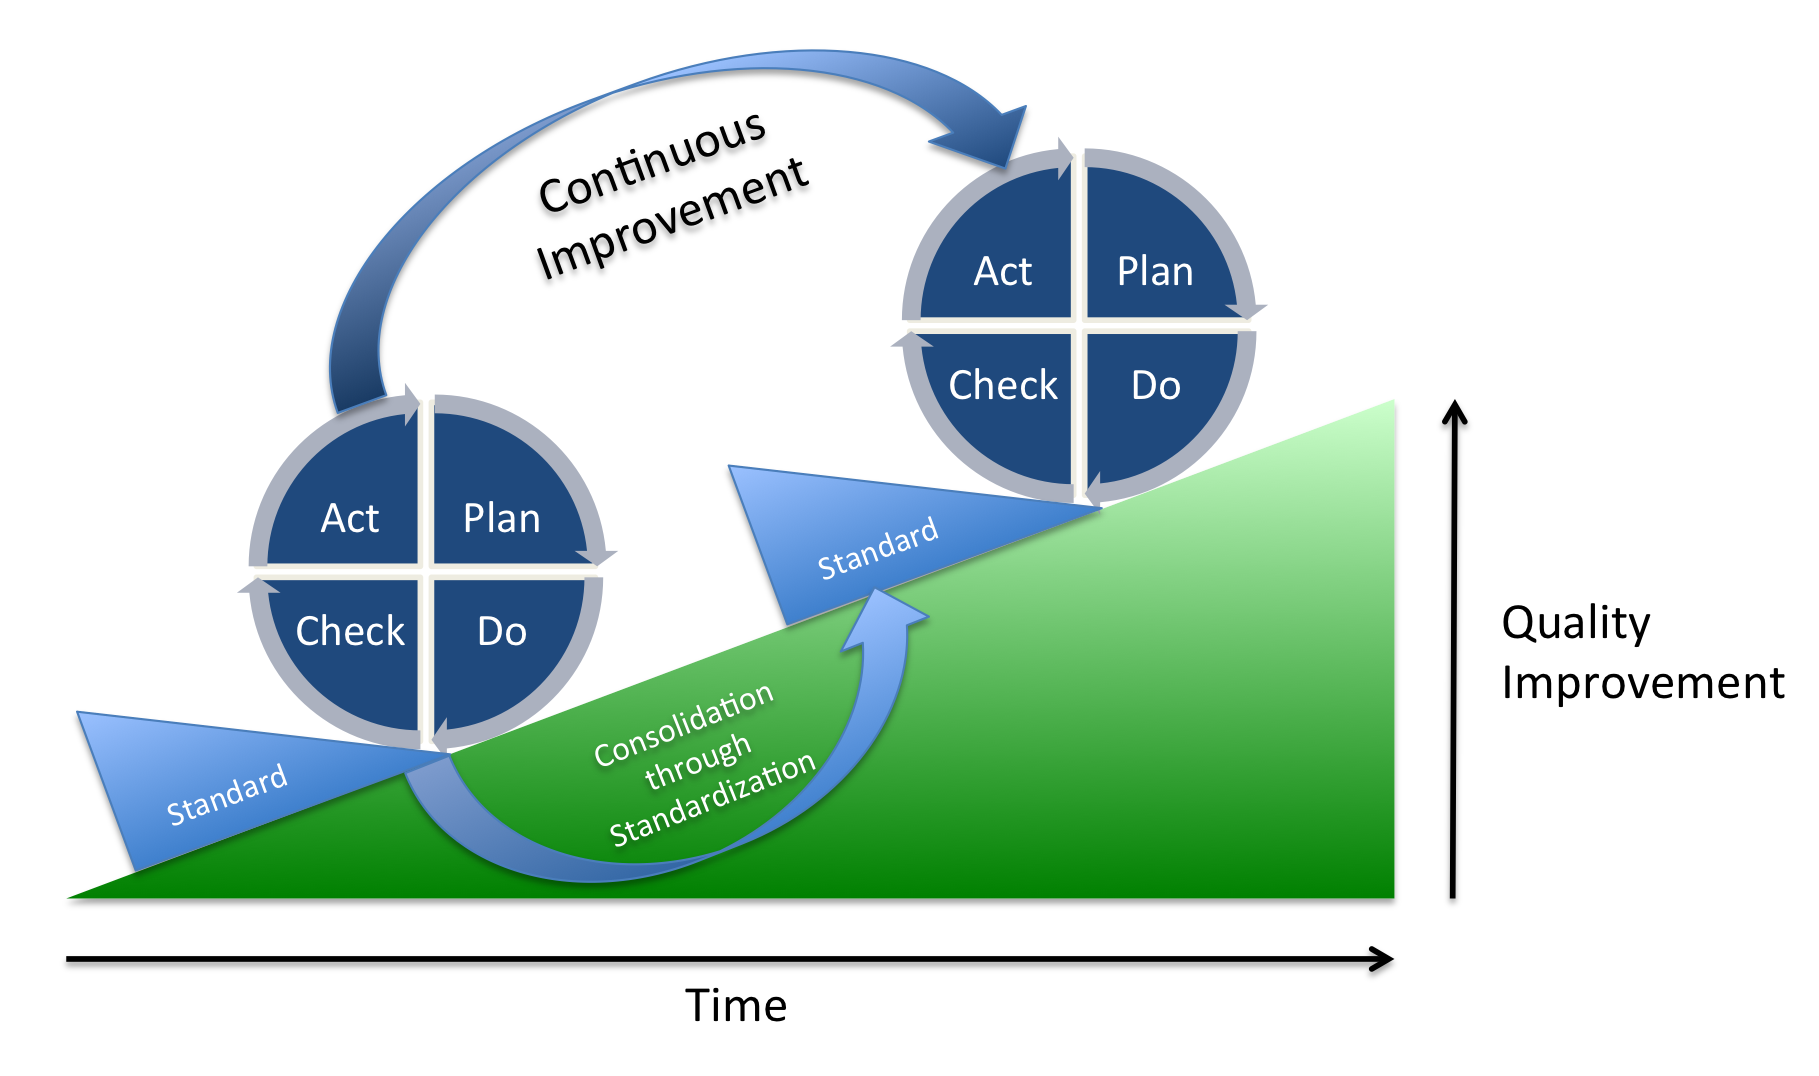
\includegraphics[scale=0.15]{ruben-tex/graphic/PDCA_Process}}
\caption{PDCA process \citep{Vietze}}
\label{fig:pdcaprocess}
\end{figure}
\noindent Genom att följa Shewhart cykeln under ett projekt kan man iterativt förbättra sin arbetsprocess och genom detta öka kvaliteten av den produkt man utvecklar, se figur \ref{fig:pdcaprocess}.
\newline
\newline
När det väl är dags för överlämning av en produkt eller tjänst är det bra att göra en kravinspektion innan. En kravinspektion enligt IEEE standarden för ''Software reviews'' syns nedan.

\begin{tcolorbox}[boxrule=1pt,leftrule=5pt,arc=0pt,auto outer arc]
\textbf{''}A process or meeting during which a software product is examined by a project personnel, managers, users, customers, user representatives, or other interested parties for comment or approval\textbf{''} \citep{SFSR}
\end{tcolorbox}

\noindent
Det man vill få gjort med en kravinspektion är alltså att produkten eller tjänsten som har tagits fram ska utvärderas av berörda parter så att den uppfyller de krav som har fastställts i ett tidigare skede för ett godkännande. En kravinspektion kan se ut som sådan \citep{Sandahl}:
\begin{enumerate}
\item{Tillträde.}
\item{Planering och översikt. Under detta steg sker en planering över hur inspektionen ska gå till och en översikt av produkten ges.}
\item{Individuell granskning. De berörda parterna granskar produkten eller tjänsten.}
\item{Möte. Efter granskningen görs en lista av alla de defekter som kan ha hittats.}
\item{Ändringar och uppföljning. I detta skede åtgärdar man de defekter som stöttes på och normalt brukar verifiera detta.}
\item{Utträde.}
\end{enumerate}

\subsection{Sammanfattning}
Sammanfattningsvis kan man konstatera att ett återkommande tema för att ta fram en högkvalitativ produkt eller tjänst är att planera, utföra och granska, för att sedan upprepa proceduren under projektets gång. Detta är dock bara en teoretisk tillämpning och verkligheten kan se annorlunda ut.

\section{Metod}
	För att ta reda på all information som behövs har ett flertal böcker blickats igenom. Ingen av dem har läst till 100\%, utan endast de intressanta delarna har läst med mer nogrannhet. För att verifiera att det som lästs stämmer har vissa delar testats i praktiken, i detta fall på projketet. Till exempel så har enhetstester körts på matris bibliotekts funktioner såsom matrisaddition, sytemtester och modultester har körts på den kvadratiska problem-lösaren och acceptanstester har körts på alla delar i projektet för att se till att alla krav är uppfyllda. Mer om detta kan läsas i resultat.
	
\subsection{Enhetstest}
	I ''Software Unit Testing'' \citep{ivv} definierar ett enhetstest som ett test på den minsta möjliga samlingen kod som fortfarande går att testa nyttofullt, alltså att koden är tillräckligt stor för att fel ska kunna uppstå. Dessa test är bra då de är riktade mot en så liten portion med kod och i och med detta sällan missar buggar och fel. Det som kan vara krångligt med enhetstest är att just hitta dessa minsta samlingarna med kod, speciellt om det är en extern part (en annan programmerare) som ska skapa och utföra testen. I och med att man kör enhetstester på så små delar av kod har de i teorin en tendens till att bli väldigt många om man ska täcka tillräckligt stor funktionalitet. Detta är dock oftast inget problem i praktiken eftersom många små funktioner ofta är triviala och har ytterst få uppgifter. Då behöver inte så många test skrivas, om ens ett enda.
\subsection{Modultest}	
	Det finns flera olika definitioner av vad en modul är, och i och med det blir det då svårt att definiera vad ett modultest är. I ''The Art of Software Testing'' definierar de att moduler och enheter är samma sak men jag har valt att istället gå efter Kristian Sandahls definiton. Han definierar att ett modultest är ett integrationtest utav två eller fler enheter. Det går ut på att man kombinerar ett antal enheter och sedan testar dem tillsammans. Testen i sig kan var väldigt lika enhetstest men täcker nu en mer komplex funktionalitet. Precis som enheter kan moduler vara svåra att definiera. Om allt för många enheter förs samman och modulen får mer funktionalitet kanske den till slut kan klassas som ett system, och då förlorar modultestningen sitt syfte. Om man har ett så litet projekt som detta så är moduldefinitionen ofta inte så svår, eftersom både komplexiteten och utvecklingsmöjligheterna är begränsade. Det är kritiskt vid dessa test att underliggande funktioner redan är testade. Om inte, kan i stort sett inga slutsatser, angående vad som är fel, dras när ett test misslyckas.
\subsection{Systemtest}	
	Ett systemtest är precis som modultest ett integrationstest, men nu utav ett antal moduler istället. Enligt ''The Art of Software Testing'' inriktar sig testet nu också vanligtvis på hela produkten som har utvecklats, för att se om funktionalitetskraven är uppfyllda. Detta för att säkerställa dess funktionalitet och för att hitta fel som uppstått vid kommunikation mellan moduler. Exempel på systemtest i vårt projekt är test av lösaren. Anledningen till att lösaren ses som ett eget system och inte är ihopbakad med GUI:t är att den ska kunna fungera separat. Givetvis är de båda ihopbakade också ett system, som också kräver systemtest.	
\subsection{Acceptanstest}	
	Ett acceptanstest är ett test som har målet att testa om programmet är acceptabelt. Med det menas att testen validerar ifall programmet uppfyller alla krav som ställs på det, och nu inte endast funktionalitetskraven. I vårt projekt är det huvudsakligen prestandan som behöver acceptanstestas. Då det prestandakrav produkten hade var relativt vagt ("Produkten ska ha likvärdig prestanda med Gurobi"), och att kravet sedan förhandlades bort, gjorde att testen inte hade så stor prioritet. Men för att få någon vetskap om produktens hastighet och för att garantera att kunden blir nöjd krävs ändå någon form utav test.
\subsection{Övrigt}	
	I projektet har även ett byggsystem använts, som smidigt kompilerat all kod automatiskt. Systemet har därefter även kört alla tester som skapats genom projektet.
	Med hjälp av byggsystemet och Kontinuerlig Integration har all kod då kunnat testas direkt när någon har skrivit ny kod och därav har det gått att se när och var feluppstått. Och eftersom systemet även har kört alla gamla test har koden säkerställts med att alla andra funktioner, de som inte har rörts, också fortfarande fungerar.
\section{Resultat}	
	Följande del beskriver hur arbetet med efterforskningen gick samt hur testen utfördes.
	\subsection{Efterforskning}
	Det finns otroligt mycket information om mjukvarutestning men samtidigt är ämnet ganska vagt då testning beror så mycket på just vad som ska testas. I vårt projekt visade det sig att ''Black Box''-testning var den metod som överlägset lämpade sig bäst. ''Black Box'' går ut på att man sätter en ''svart låda'' över det som ska testas, så att man endast kan se in- och utdatan. Sedan tittar man på utdata och ser ifall den är den förväntade. ''Black Box'' anses bra i detta projekt eftersom hela Quadopt är uppbyggd utav många små funktioner och resultateten som de ska ge tillbaka är oftast kända på förhand. Ett exempel på detta är matrisaritmetiken där resultatet, av till exempel en multiplikation, går att räkna ut ganska enkelt på papper. Enligt ''The Art of Software Testing'' ska dessa test utgå ifrån kravspecifikationen och andra dokument som beskriver vad produkten ska ha för funktionalitet. Boken beskriver också ''Black Box'' som en utmattande testteknik. Med det menar de att man borde testa alla möjliga indata till den svarta lådan och se så att svaren stämmer. Detta är precis som det står i boken i praktiken omöjligt. Speciellt i vårt projekt där det enda som begränsar antalet olika sätt en matris, bestående utav tal, kan se ut på är datorns minne. \newline
I projektet fanns dock ofta behovet av se en funktions lösningsgång, och då är ''Black Box'' en väldigt dålig metod. En metod som då lämpar sig bättre är ''White Box'' testning, som innebär att man tittar på den interna strukturen i en funktion. Därefter kan man se, efter vald indata, om lösningsgången är den väntade. I ''The Art of Software Testing'' står det att även denna metod kan problematisk då antalet lösningsgångar kan vara väldigt många. För att se om det ens är rimligt att utföra dessa test kan man se på funktionens cyklomatiska komplexitet. Cyklomatisk komplexitet innebär att man gör en graf över funktionen där de möjliga stadierna i lösningsgången är noder, och de möjliga lösningsvägarna är bågar. I ''Structured testing'' \citep{structest} står det att om denna komplexitet är för stor ökar antalet fel som programmeraren gjort väldigt fort, och samtidigt blir det i stort sett omöjligt att utföra några ''White Box''-test då fel kan uppstå på så många ställen. \\ 	
För att säkerställa projektets krav behövdes bara en testmetod till, och det var en metod för att mäta prestanda. Den som valdes var ''Load testing'' som innebär att man belastar programmet med mycket data och ser hur bra det fungerar. I projektets fall gavs lösaren många problem och tittade på hur fort det gick i förhållande till andra lösare. \newline	
Det skulle kunnat varit så att GUI:t hade haft högre prioritet än vad det hade. I det fallet hade olika typer av UX- och användartest varit nödvändiga för att kvalitetssäkra produkten. Men eftersom GUI:t beställdes utifrån kundens personliga behov, var det tydligt definierat redan från början att det var av låg prioritet. 
	
	\subsection{Praktik}
	Som beskrivet tidigare finns det i stort sett oändligt många kombinationer av in- och utdata.	För att då kunna utföra ''Black Box''-testerna behövdes antalet testfall reduceras. Detta åstadkoms genom att ha möten med kunden som klargjorde att indata till programmet alltid skulle vara giltig. Det reducerade antal testfall enormt mycket, men som beskrivet i resultatet av efterforskningen finns det även väldigt mycket giltig indata. Exempelvis för matrisaritmetiken. Dessa test gick också att reducera genom att de flesta operationer är triviala och endast kräver numeriska test såsom nolldivision och flyttalsfel. Genom att även utnyttja ''White Box''-tekniken gick det att utforma olika ''Black Box''-test som tog olika vägar genom koden och på så sätt bara skapa ett test för varje väg. Denna teknik utnyttjades endast på mindre funktioner såsom moduler för att antalet olika fall skulle begränsas till något som var rimligt. \newline
	För lösaren gick det att applicera samma metod, eftersom dess funktionalitet bygger mycket på underliggande funktioner. Det som skilde sig gentemot småfunktionerna var att nu behandlades oftast rader eller kolumner i matriser istället för enskilda element. Detta ledde till att de flesta test kontrollerade på kanterna utav det tillåtna området. Alltså kunde ett test vara att försöka hämta ut en radvektor på rad -1 ur en matris, vilket skulle vara ogiltigt.\newline
Vid granskning av testresultat från Git, Travis (verktyg för Kontinuerlig integration) och gruppmedlemmar visade det sig att majoriteten fel av bestod utav två typer: ''Assertion''s som misslyckats och ''Segmentation fault''. En ''Assertion'' är ett test inuti koden som avbryter exekveringen om testet inte går bra. ''Segmentation fault'' är ett programmeringsfel som resulterat i en ogiltig läsning eller skrivning till minnet. Felen som uppstod var väldigt utspridda och olika. Det som de flesta hade gemensamt var dock att de låg på en låg nivå, alltså i bottenfunktionerna. \newline	
	För att testa algoritmens hastighet stötte gruppen på oväntade problem, lösarna var för snabba.	Då varje testkörning tog 0.00 sekunder för alla lösarna förutom MATLAB behövdes testen köras många gånger för att se en tydlig skillnad. Anledningen till att MATLAB är långsammare är för att den är oerhört generell men förmodligen inte gjorts med fokus på att vara snabb. Gurobi är snabb eftersom dess enda uppgift är att lösa sådana här problem och har arbetats på under lång tid. Vår algoritm är snabb eftersom den inte är generell, alltså bryr vi oss inte om vissa specialfall som vi aldrig kommer stöta på. \newline
	För att då testa deras prestanda fick lösarna lösa olika optimeringsproblem många gånger, ofta upp emot 1000 gånger, för att kunna skilja deras egentliga hastighet. Att köra testen på vår lösare och i MATLAB var enkelt då vi hade funktionalitet för att konvertera matriser från MATLABs definition till vår, och vice versa. Däremot så var det krångligare i gurobi eftersom tiden som var allokerad för utbildning av programmet var begränsad. Det tvingade gruppen till att mata in problemet på ekvationsform vilket gjorde att gruppmedlemmarna var tvungna att köra endast små tester. Redan vid problem med fler än 10 bivillkor skulle det ta väldigt lång tid att konvertera och mata in problemet. \newline
	
	
	\subsection{Enhetstester}
	Under projektet har många enhetstest skrivits (framförallt för matrisbiblioteket). Dessa test har skrivits innan och under kodningen och sedan utförts direkt efter att koden blivit klar. Det som var intressant med dessa test var mängden av fel som upptäcktes direkt. Det ledde till att utvecklingen blev mycket effektiv då fel kunde åtgärdas direkt.
	
	\subsection{Integrationstester}
	De modultester som planerades och utfördes under projektet var framförallt lösarens funktioner. Modulerna var uppbyggda utav sammansättningar av enheter från matrisbiblioteket och andra strukturer. Dessa test utfördes vanligtvis samtidigt som implementeringen pågick. Detta för att hela tiden se till att rätt protokoll och gränssnitt användes.\\
De systemtester som utförts är tester utav lösaren och subproblemslösaren. Dessa ansågs vara tillräcklig komplexa för att ses som system. 
	
	
	\subsection{Acceptanstester}
	De acceptanstester som utförts under projektet är framförallt prestandatester. Detta då det enda kravet lösaren hade var att den skulle vara ungefär lika snabb som den kommersiella lösaren Gurobi. Då detta krav sedan togs bort lade mindre energi på prestandatester. Men de delar som ändå testats var framförallt underfunktioner till lösaren, såsom matrisbiblioteket och subproblemslösaren.
	
	\subsection{Misstag}
	Det hände att vissa modul- och systemtester skedde innan de underliggande enheterna blivit testade. Ett exempel på det är lösaren, som gruppen ivrigt ville få igång och började därför testa den tidigt. Då den inte fungerade korrekt gjorde detta att det tog lång tid att hitta felen som förmodligen hade upptäckts mycket snabbare om bara rätt testprocess hade använts.
	
	
\section{Diskussion}
Under denna del kommer en diskussion angående om resultaten ske samt metoderna som användes.
\subsection{Resultat}
Resultaten för alla tre punkter måste anses vara rimliga. Den första punkten angående vad som är rätt nivå är en väldigt diffus fråga och kan bara svaras genom att båda parter, dvs leverantör och kund har ett enhetligt svar. Eftersom det man kommer överens om i en eventuell kravspecifikation måste räcka att fullfölja för att det ska klassas som rätt nivå gällande kvalité. Sen om kunden hade velat haft några andra funktioner med produkten eller tjänsten så borde kunden ha specificerat detta. Leverantörer har också skyldighet att försöka uppfylla alla krav som har specificerats på ett snyggt sätt och inte bara slänga ihop något som fungerar, små detaljer kan utmärka ett arbete.
\newline
\newline
Den andra punkten finns det inte mycket att diskutera om, som allt annat i livet krävs det struktur för att man ska uppnå något. Under teoridelen i kapitel tre kan man konstatera att planera, utföra och granska antagligen kommer generera en produkt eller tjänst av tillräckligt god kvalité.
\newline
\newline
Angående den sista punkten kan man byta svaret från ett ja till ett nej, då ett krav förhandlades bort. I detta projekt hade kandidatgruppen endast ett mätbart krav, detta krav specificerade att optimeringsalgoritmen skulle vara likvärdig i hastighet i jämförelse med en kommersiell mjukvara kallad ''Gurobi''. ''Gurobi'' specialiserar sig i att lösa olika sorters optimeringsproblem \citep{gurobi}. Under projektets slutskede diskuterade kandidatgruppen med kunden om att det kommer bli svårt att vara jämbördig med ''Gurboi'', detta var inget problem för kunden och kravet kunde tas bort. Kunden tryckte på att det viktigaste var att koden fungerar och att den är väldokumenterad, vilket den är. Däremot kan jag tycka att om man tar bort ett krav så har man misslyckats och därför anser jag att man kan ändra svaret till nej, slutprodukten håller inte tillräckligt god kvalité, men då är jag väldigt hård mot mig själv och kandidatgruppen. Däremot säger teorin bakom det hela att produkten håller tillräckligt god nivå då den uppfyller alla krav, det ska inte spela någon roll om man har förhandlat bort något krav eller inte.

\subsection{Metod}
Efter slutförandet av projektet och analys av hur det hela gick finns det många saker man hade kunnat gjort annorlunda. Ett återkommande problem som stöttes på under projektets gång var att kodstandarden som hade satts upp från början inte följdes helt och hållet, inte förens den sista iterationen skrevs kod efter den. Detta resulterade i att mycket tid lades ner på att refaktorera kod. Kodstandarden innehöll inte heller allt som bör ta hänsyns till. Ett exempel är att frigöra minne, vilket resultera i att mycket tid lades ner på att hitta och åtgärda minnesläckor. Eftersom kandidatgruppen hade ett krav på att skriva pålitlig kod så är förstås minnesläckor inte accepterbart. 
\newline
\newline
Jag tror att slutprodukten skulle ha sett annorlunda ut om kodstandarden täckte fler områden i hur man ska skriva kod samt om man tryckte på hur viktigt det är att följa kodstandarden. Jag som kvalitetsamordnare hade kunnat trycka mer på att kodstandarden skall följas för att en produkt av bättre kvalité skulle skapats.
\newline
\newline
I teoridelen visade forskningen att om man ska uppnå en högkvalitativ produkt kan man t.ex. använda sig av Shewhart cykeln, planera, göra, studera och agera. Kandidatgruppen planera hur man skulle skriva kod, man följde inte kodstandarden, kandidatgruppen var väl medveten om det. Vid detta stadiet borde man agera, visserligen sas det åt folk att börja använda kodstandarden, men det hade nog varit bättre att utvärdera om kodstandarden och föra dialog om varför den inte följs för att skriva en ny som möjligtvis alla känner sig bekväma med.

\section{Slutsatser}
{\LaTeX} lämpar sig mycket väl för teknisk dokumentation i ett programmeringsprojekt. Denna slutsats kan dras från det {\LaTeX} dokument gruppen har producerat. {\LaTeX} gav oss verktygen för att infoga figurer, matematiska formler, ekvationer, algoritmer och pseudokod som behövdes för dokumenten i projektet.   
\newline
\newline
Det tog hela projekttiden för att samtliga medlemmar skulle känna att de behärskade {\LaTeX}. Detta kan ses som en lång inlärningskurva för språket och att det tog onödig tid från andra delar av projektet. Dock var detta aldrig egentligen något problem, mycket hjälp fanns att hämta från internet och då två av gruppmedlemmarna behärskade {\LaTeX} sedan tidigare kunde de hjälpa och lära resten av gruppen. 
\newline
\newline
Om ingen av gruppens medlemmar hade använt {\LaTeX} sedan tidigare kan det diskuteras om det hade varit lönsamt för gruppen att lära sig det. Då hade mer tid behövts läggas på utbildning av språket och andra uppgifter hade fått lida. Som sagt lämpar sig {\LaTeX} mycket väl för teknisk dokumentation i ett programmeringsprojekt och även om det hade tagit mer tid så hade det varit värt i det långa loppet.    
\newpage

%Johans report
\newpage
\stopcontents[sections]
\resumecontents[default]
\addcontentsline{toc}{section}{\protect\numberline{E} Mjukvarutestning}
\stopcontents
\startcontents[sections]
\LIPSTitelsidajohan
\setcounter{section}{0} 
\printcontents[sections]{ }{1}{}
\newpage
\section{Inledning}
Jag har gjort en filhanterar som visualiserar alla filer och mappar i 3D med hjälp av OpenGL. Inspirationen till detta projekt var bland annat FSN (File System Navigator) som gjordes av SGI för IRIX systemen och FSV(File System Visualizer) som är en remake av FSN på Linux, se figur~\ref{fig:fsn}. En annan inspiration var det lite modernare TDFSB som även visar upp bilder och filmer i 3D världen, se figur~\ref{fig:tdfsb}. 

\begin{center}
\begin{figure}[H]
    \centering
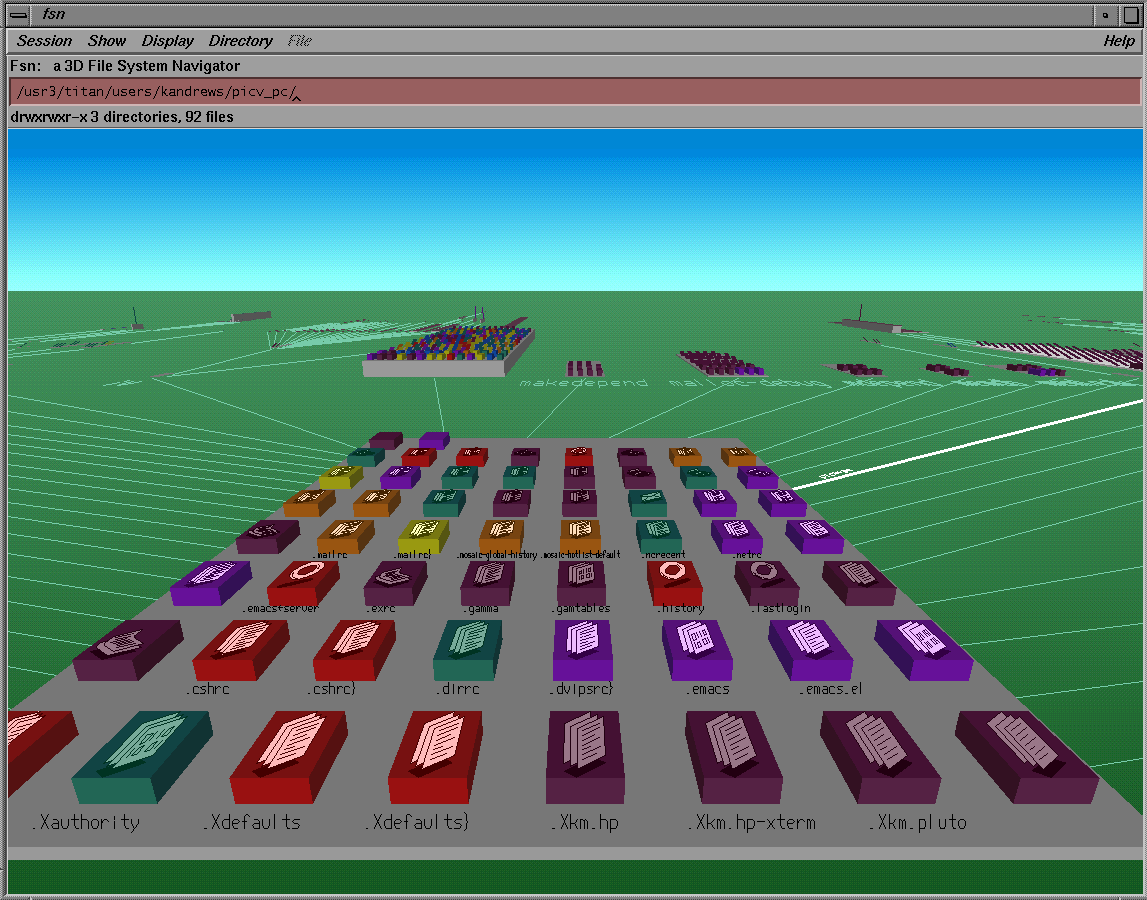
\includegraphics[width=8cm]{../grafik/fsn1.png}
\caption{FSN.}
\label{fig:fsn}
\end{figure}
\end{center}

\begin{center}
\begin{figure}[H]
    \centering
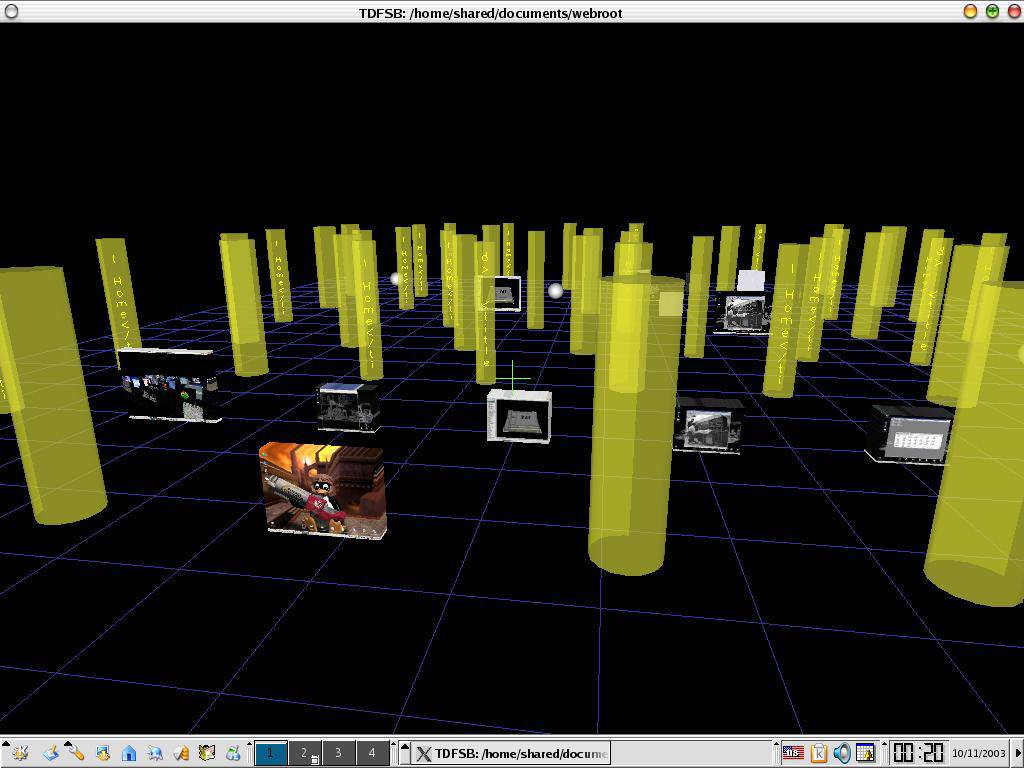
\includegraphics[width=8cm]{../grafik/tdfsb.jpg}
\caption{TDFSB.}
\label{fig:tdfsb}
\end{figure}
\end{center}

De ursprungliga obligatoriska kraven för produkten var följande:
\begin{LIPSkravlista}
\LIPSkrav{Original}{Alla filer ska representeras av block med någon textur på, är det en bild så ska bilden användas som textur}{1}

\LIPSkrav{Original}{Alla mappar ska representeras av block med någon textur}{1}
\LIPSkrav{Original}{Alla mappar och filer i en mapp ska vara placerade på en platta med en textur}{1}
\LIPSkrav{Original}{Ljussättningen ska ske med en Phong-shader}{1}
\LIPSkrav{Original}{Alla block ska ha skuggor}{1}
\LIPSkrav{Original}{Navigeringen ska vara first person där piltangenterna styr x och z koordinaterna och musen styr kameren i ett sfäriskt koordinatsystem}{1}
\LIPSkrav{Original}{Man ska inte kunna gå igenom filerna(collisions detection)}{1}
\LIPSkrav{Original}{Du ska kunna gå in i en mapp så transporteras du till den nya mappen)}{1}
\LIPSkrav{Original}{Du ska kunna klicka på en fil/mapp och få upp alla möjliga alternativ såsom radera, öppna...)}{1}
\LIPSkrav{Original}{Om du raderar en fil ska övriga filer ordna sig så det inte är några luckor någonstans}{1}
\LIPSkrav{Original}{Skydome ska finnas}{1}
\LIPSkrav{Original}{Endast Linux kommer stödjas}{1}
\end{LIPSkravlista}


och de ej obligatoriska kraven var följande:
\begin{LIPSkravlista}
\LIPSkrav{Original}{Du ska kunna få upp en terminal i filhanteraren}{2}
\LIPSkrav{Original}{Du ska kunna klicka på en mapp och sedan få upp en portal som du kan se in i mappen genom}{2}
\LIPSkrav{Original}{När du raderar en fil ska den explodera}{2}
\LIPSkrav{Original}{Innehåller en mapp många filer/mappar ska frustum culling användas för att minimera beräkningar}{2}
\LIPSkrav{Original}{Mapparnas texturer ska vara den ikon filen som operativsystemet använder med transparens, då ska renderingsordningen och vara korrekt}{2}
\end{LIPSkravlista}
Under projektets gång gick de obligatoriska kraven igenom en modifikation på grund av att projektet tog längre tid än vad jag trodde samt att en del inte riktigt passade in. Krav 5 togs bort på grund av tidsbrist, krav 6 gjordes om så att användaren bara navigerade i XZ planet då detta passade mycket bättre samt en del förenklingar kunde göras. Krav 9 togs bort då en terminal ansågs vara mycket enklare att implementera så all modifikation av filsystemet görs via den. Inga av de ej obligatorska kraven uppfylldes på grund av tidsbrist. I figur~\ref{fig:tmbtrf} kan man se resultatet. 
\begin{center}
\begin{figure}[H]
    \centering
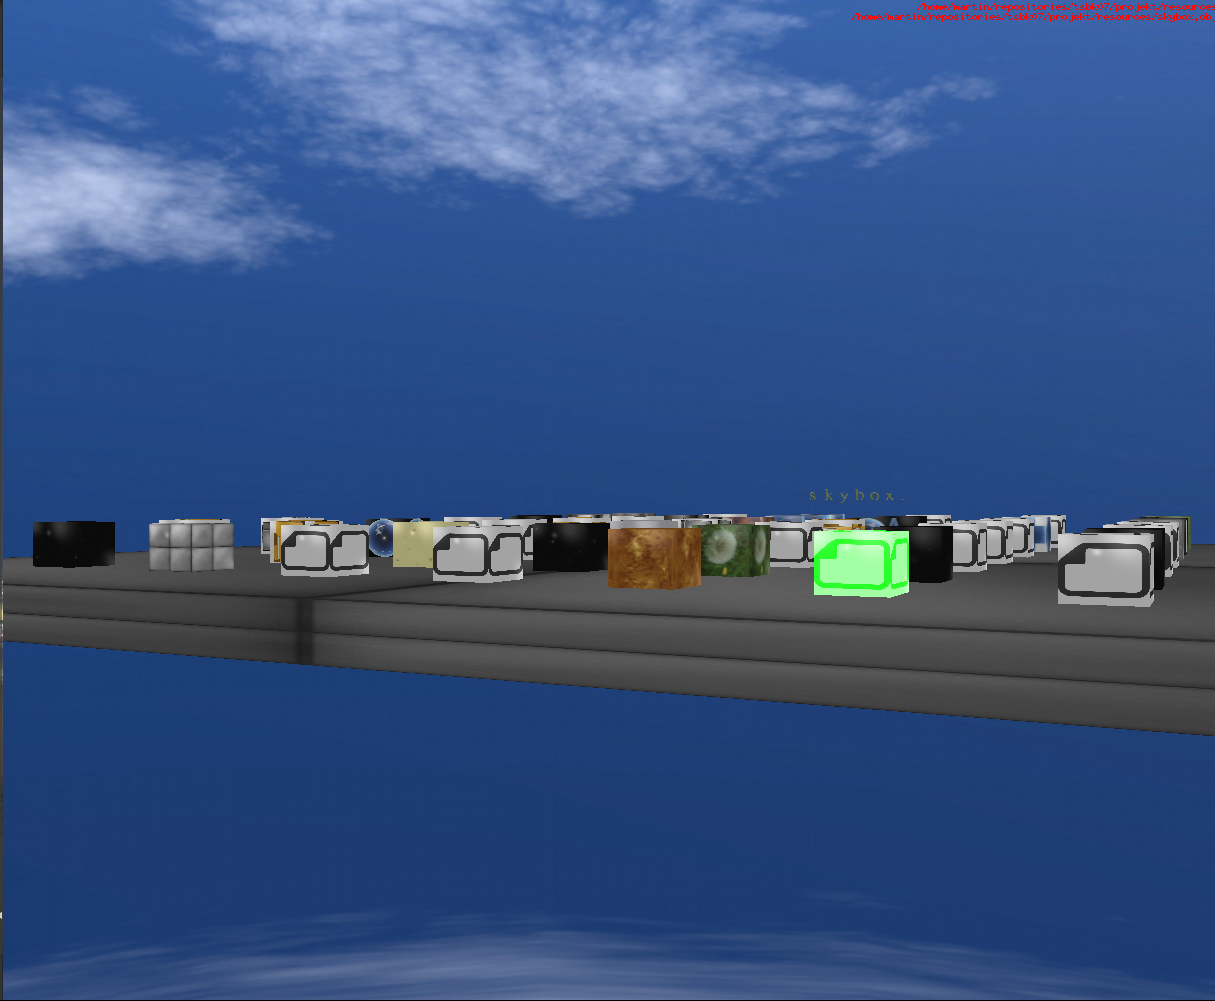
\includegraphics[width=8cm]{../grafik/tmbtrf.png}
\caption{TMBTRF.}
\label{fig:tmbtrf}
\end{figure}
\end{center}

\section{Bakgrund}
Det svåraste problemet jag hade innan jag började med projeketet var att på ett effektivt sätt interagera med datorns filsystem. Detta löstes rätt enkelt när jag upptäckte Boost::Filesystem. Detta bibliotek är inte speciellt använt så det finns inte så mycket hjälp att hitta på forum men dokumentation för det är väldigt bra så när jag väl kom in i det så fungera det väldigt bra. Funktioner såsom att byta namn och radera filer fanns redan implementerade så detta underlättade mycket.
\\
\\
Ett annat problem som var svårare än vad jag trodde var att visa filnamn i en 3D miljö. Den enklaste lösning skulle varit att använda något bibliotek för att generera texturer med en font till exempel FreeType. Jag försökte detta och jag kommer inte ihåg varför men jag fick det inte att fungera. För att få detta snyggt så skulle texturerna behöva vara transparenta så jag skulle behöva ta hänsynt till ordningen som alla objekt renderas. Min lösning på problemet var att generera .obj filer för alla tänkbara bokstäver och tecken som kan förekomma i ett filnamn. Jag valde alla bokstäver a-z och A-Z, alla siffror samt tecknen . - \_. Detta gjordes med ett python script i cad-programmet FreeCad. För att minimera inläsningstiden så läses alla dessa modeller in vid starten av programmet och återanvänds hela tiden. För att undvika problem som kan uppkomma vid långa filnamn som sträcker sig över hela miljön så visas bara de 7 första tecknen i filnamnet.
\\
\\
Anledningen till att C++ valdes var mest för dess datastrukturer såsom Vector, Map och string. Allting som kan göras i C++ kan självklart göras i C men där så är allting klart. Detta gjorde så att jag kunde göra en väldigt allmän klass som representerar alla objekt i 3D världen. Programmet arbetar också mycket med strängar och då är String väldigt mycket smidigare än en char array.
\\
\\
Ett problem som upptäcktes senare var att när man går in i en mapp som innehåller många filer, speciellt bilder, så tar det rätt lång tid innan hela världen har genererats. Detta skulle kunna lösas genom att ha en separat tråd som förbereder alla undermappar i den nuvarande mappen. Detta har dock inte implementeras men skulle jag fortsätta utveckla TMBTRF så skulle detta vara ett av de första problemen jag skulle lösa. 

\section{Teori}
I boken ''Software Product Quality Control'' \citep{SPQC} nämns ett antal definitioner som förtydligar vad kvalitetssäkring innebär, dessa syns nedan.  

\begin{itemize}
  \item ''Quality assurance: a planned and systematic pattern of all actions necessary to provide adequate confidence that an item or product conforms to established technical requirements.'' \citep[p.19]{SPQC} 
  \item ''Constructive quality assurance: All means to be used in constructing a product in a way so it meets its quality requirements.'' \citep[p.19]{SPQC} 
  \item ''Analyctical quality assurance: All means of analysing the state of the quality of a product.'' \citep[p.19]{SPQC} 
\end{itemize}
\noindent Kvalitetssäkring innebär följaktligen att man som leverantör av en produkt eller tjänst ska se till att de uppfyller de krav som har satts upp i en eventuell kravspecifikation. Det är dessa krav som sätter standarden för vad som är rätt nivå gällande kvalité. Under arbetsgången måste man analysera om man är på väg att uppfylla kraven eller inte, i sådana fall måste detta åtgärdas omedelbart.
\newline
\newline
Med detta sagt finns det flera steg i ett projekt att kvalitetssäkra. Ett effektivt sätt att göra detta på är genom att följa Shewhart cykeln, det vill säga planera, göra, studera och agera (PGSA) \citep{PDCA}. Shewhart cykeln är en iterativ fyra stegs metod, se figur \ref{fig:shewcycle}. Metoden är utvecklad av William Edwards Deming. Namnet ''Shewhart'' kommer från en av Demings kollegor \citep[p.~88]{Deming}. 
\begin{figure}[h]
\centerline{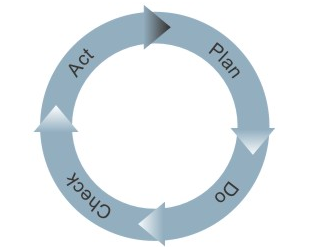
\includegraphics[scale=0.5]{ruben-tex/graphic/shewhartcycle}}
\caption{Shewhart cykeln \citep{Mindtools}}
\label{fig:shewcycle}
\end{figure}
\begin{enumerate}
  \item Planera. I detta skede ska målet fastställas, det vill säga sätta upp de krav som behövs för att kunden skall bli nöjd. Genom att göra detta är det tydligt om vad som skall göras och en överenskommelse finns mellan kund och leverantör. 
  \item Göra. När man konstaterat vad som behöver göras för att kunden skall bli nöjd är det dags att implementera ett sätt att arbeta och fullfölja processen.
  \item Studera. Efter att ha följt processen under en viss period är det dags att utvärdera om processen man har följt kommer leda till att man uppfyller de målen man har fastställt i planeringsfasen.
  \item Agera. Om man under studeringsfasen upptäcker att processen man följer inte kommer leda till att man uppfyller de krav som kund och leverantör var överens om måste detta åtgärdas omedelbart genom att planera om arbetsprocessen eller i viss mån diskutera kraven med kunden. Om processen som följs kommer uppfylla de krav som har satts upp kan man fortsätta med iterationerna av Shewhart cykeln precis som innan.
\end{enumerate}
\begin{figure}[h]
\centerline{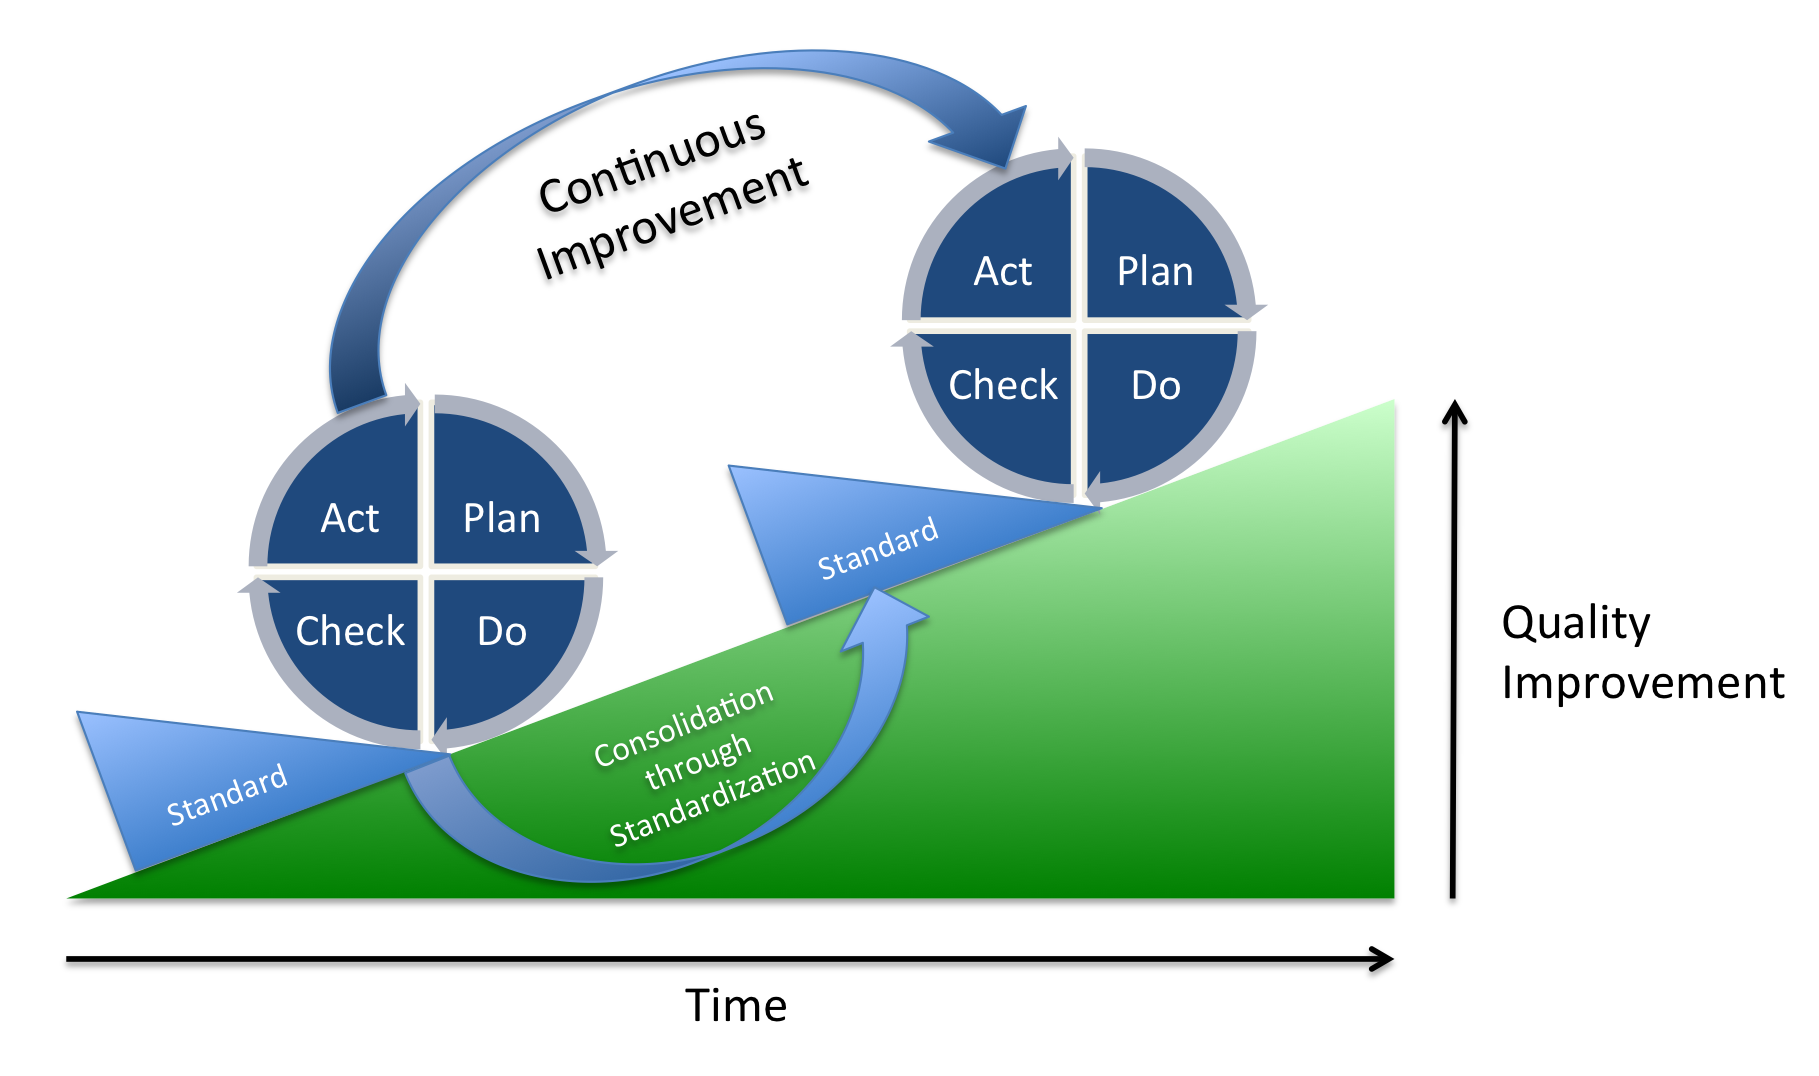
\includegraphics[scale=0.15]{ruben-tex/graphic/PDCA_Process}}
\caption{PDCA process \citep{Vietze}}
\label{fig:pdcaprocess}
\end{figure}
\noindent Genom att följa Shewhart cykeln under ett projekt kan man iterativt förbättra sin arbetsprocess och genom detta öka kvaliteten av den produkt man utvecklar, se figur \ref{fig:pdcaprocess}.
\newline
\newline
När det väl är dags för överlämning av en produkt eller tjänst är det bra att göra en kravinspektion innan. En kravinspektion enligt IEEE standarden för ''Software reviews'' syns nedan.

\begin{tcolorbox}[boxrule=1pt,leftrule=5pt,arc=0pt,auto outer arc]
\textbf{''}A process or meeting during which a software product is examined by a project personnel, managers, users, customers, user representatives, or other interested parties for comment or approval\textbf{''} \citep{SFSR}
\end{tcolorbox}

\noindent
Det man vill få gjort med en kravinspektion är alltså att produkten eller tjänsten som har tagits fram ska utvärderas av berörda parter så att den uppfyller de krav som har fastställts i ett tidigare skede för ett godkännande. En kravinspektion kan se ut som sådan \citep{Sandahl}:
\begin{enumerate}
\item{Tillträde.}
\item{Planering och översikt. Under detta steg sker en planering över hur inspektionen ska gå till och en översikt av produkten ges.}
\item{Individuell granskning. De berörda parterna granskar produkten eller tjänsten.}
\item{Möte. Efter granskningen görs en lista av alla de defekter som kan ha hittats.}
\item{Ändringar och uppföljning. I detta skede åtgärdar man de defekter som stöttes på och normalt brukar verifiera detta.}
\item{Utträde.}
\end{enumerate}

\subsection{Sammanfattning}
Sammanfattningsvis kan man konstatera att ett återkommande tema för att ta fram en högkvalitativ produkt eller tjänst är att planera, utföra och granska, för att sedan upprepa proceduren under projektets gång. Detta är dock bara en teoretisk tillämpning och verkligheten kan se annorlunda ut.

\section{Metod}
	För att ta reda på all information som behövs har ett flertal böcker blickats igenom. Ingen av dem har läst till 100\%, utan endast de intressanta delarna har läst med mer nogrannhet. För att verifiera att det som lästs stämmer har vissa delar testats i praktiken, i detta fall på projketet. Till exempel så har enhetstester körts på matris bibliotekts funktioner såsom matrisaddition, sytemtester och modultester har körts på den kvadratiska problem-lösaren och acceptanstester har körts på alla delar i projektet för att se till att alla krav är uppfyllda. Mer om detta kan läsas i resultat.
	
\subsection{Enhetstest}
	I ''Software Unit Testing'' \citep{ivv} definierar ett enhetstest som ett test på den minsta möjliga samlingen kod som fortfarande går att testa nyttofullt, alltså att koden är tillräckligt stor för att fel ska kunna uppstå. Dessa test är bra då de är riktade mot en så liten portion med kod och i och med detta sällan missar buggar och fel. Det som kan vara krångligt med enhetstest är att just hitta dessa minsta samlingarna med kod, speciellt om det är en extern part (en annan programmerare) som ska skapa och utföra testen. I och med att man kör enhetstester på så små delar av kod har de i teorin en tendens till att bli väldigt många om man ska täcka tillräckligt stor funktionalitet. Detta är dock oftast inget problem i praktiken eftersom många små funktioner ofta är triviala och har ytterst få uppgifter. Då behöver inte så många test skrivas, om ens ett enda.
\subsection{Modultest}	
	Det finns flera olika definitioner av vad en modul är, och i och med det blir det då svårt att definiera vad ett modultest är. I ''The Art of Software Testing'' definierar de att moduler och enheter är samma sak men jag har valt att istället gå efter Kristian Sandahls definiton. Han definierar att ett modultest är ett integrationtest utav två eller fler enheter. Det går ut på att man kombinerar ett antal enheter och sedan testar dem tillsammans. Testen i sig kan var väldigt lika enhetstest men täcker nu en mer komplex funktionalitet. Precis som enheter kan moduler vara svåra att definiera. Om allt för många enheter förs samman och modulen får mer funktionalitet kanske den till slut kan klassas som ett system, och då förlorar modultestningen sitt syfte. Om man har ett så litet projekt som detta så är moduldefinitionen ofta inte så svår, eftersom både komplexiteten och utvecklingsmöjligheterna är begränsade. Det är kritiskt vid dessa test att underliggande funktioner redan är testade. Om inte, kan i stort sett inga slutsatser, angående vad som är fel, dras när ett test misslyckas.
\subsection{Systemtest}	
	Ett systemtest är precis som modultest ett integrationstest, men nu utav ett antal moduler istället. Enligt ''The Art of Software Testing'' inriktar sig testet nu också vanligtvis på hela produkten som har utvecklats, för att se om funktionalitetskraven är uppfyllda. Detta för att säkerställa dess funktionalitet och för att hitta fel som uppstått vid kommunikation mellan moduler. Exempel på systemtest i vårt projekt är test av lösaren. Anledningen till att lösaren ses som ett eget system och inte är ihopbakad med GUI:t är att den ska kunna fungera separat. Givetvis är de båda ihopbakade också ett system, som också kräver systemtest.	
\subsection{Acceptanstest}	
	Ett acceptanstest är ett test som har målet att testa om programmet är acceptabelt. Med det menas att testen validerar ifall programmet uppfyller alla krav som ställs på det, och nu inte endast funktionalitetskraven. I vårt projekt är det huvudsakligen prestandan som behöver acceptanstestas. Då det prestandakrav produkten hade var relativt vagt ("Produkten ska ha likvärdig prestanda med Gurobi"), och att kravet sedan förhandlades bort, gjorde att testen inte hade så stor prioritet. Men för att få någon vetskap om produktens hastighet och för att garantera att kunden blir nöjd krävs ändå någon form utav test.
\subsection{Övrigt}	
	I projektet har även ett byggsystem använts, som smidigt kompilerat all kod automatiskt. Systemet har därefter även kört alla tester som skapats genom projektet.
	Med hjälp av byggsystemet och Kontinuerlig Integration har all kod då kunnat testas direkt när någon har skrivit ny kod och därav har det gått att se när och var feluppstått. Och eftersom systemet även har kört alla gamla test har koden säkerställts med att alla andra funktioner, de som inte har rörts, också fortfarande fungerar.
\section{Resultat}	
	Följande del beskriver hur arbetet med efterforskningen gick samt hur testen utfördes.
	\subsection{Efterforskning}
	Det finns otroligt mycket information om mjukvarutestning men samtidigt är ämnet ganska vagt då testning beror så mycket på just vad som ska testas. I vårt projekt visade det sig att ''Black Box''-testning var den metod som överlägset lämpade sig bäst. ''Black Box'' går ut på att man sätter en ''svart låda'' över det som ska testas, så att man endast kan se in- och utdatan. Sedan tittar man på utdata och ser ifall den är den förväntade. ''Black Box'' anses bra i detta projekt eftersom hela Quadopt är uppbyggd utav många små funktioner och resultateten som de ska ge tillbaka är oftast kända på förhand. Ett exempel på detta är matrisaritmetiken där resultatet, av till exempel en multiplikation, går att räkna ut ganska enkelt på papper. Enligt ''The Art of Software Testing'' ska dessa test utgå ifrån kravspecifikationen och andra dokument som beskriver vad produkten ska ha för funktionalitet. Boken beskriver också ''Black Box'' som en utmattande testteknik. Med det menar de att man borde testa alla möjliga indata till den svarta lådan och se så att svaren stämmer. Detta är precis som det står i boken i praktiken omöjligt. Speciellt i vårt projekt där det enda som begränsar antalet olika sätt en matris, bestående utav tal, kan se ut på är datorns minne. \newline
I projektet fanns dock ofta behovet av se en funktions lösningsgång, och då är ''Black Box'' en väldigt dålig metod. En metod som då lämpar sig bättre är ''White Box'' testning, som innebär att man tittar på den interna strukturen i en funktion. Därefter kan man se, efter vald indata, om lösningsgången är den väntade. I ''The Art of Software Testing'' står det att även denna metod kan problematisk då antalet lösningsgångar kan vara väldigt många. För att se om det ens är rimligt att utföra dessa test kan man se på funktionens cyklomatiska komplexitet. Cyklomatisk komplexitet innebär att man gör en graf över funktionen där de möjliga stadierna i lösningsgången är noder, och de möjliga lösningsvägarna är bågar. I ''Structured testing'' \citep{structest} står det att om denna komplexitet är för stor ökar antalet fel som programmeraren gjort väldigt fort, och samtidigt blir det i stort sett omöjligt att utföra några ''White Box''-test då fel kan uppstå på så många ställen. \\ 	
För att säkerställa projektets krav behövdes bara en testmetod till, och det var en metod för att mäta prestanda. Den som valdes var ''Load testing'' som innebär att man belastar programmet med mycket data och ser hur bra det fungerar. I projektets fall gavs lösaren många problem och tittade på hur fort det gick i förhållande till andra lösare. \newline	
Det skulle kunnat varit så att GUI:t hade haft högre prioritet än vad det hade. I det fallet hade olika typer av UX- och användartest varit nödvändiga för att kvalitetssäkra produkten. Men eftersom GUI:t beställdes utifrån kundens personliga behov, var det tydligt definierat redan från början att det var av låg prioritet. 
	
	\subsection{Praktik}
	Som beskrivet tidigare finns det i stort sett oändligt många kombinationer av in- och utdata.	För att då kunna utföra ''Black Box''-testerna behövdes antalet testfall reduceras. Detta åstadkoms genom att ha möten med kunden som klargjorde att indata till programmet alltid skulle vara giltig. Det reducerade antal testfall enormt mycket, men som beskrivet i resultatet av efterforskningen finns det även väldigt mycket giltig indata. Exempelvis för matrisaritmetiken. Dessa test gick också att reducera genom att de flesta operationer är triviala och endast kräver numeriska test såsom nolldivision och flyttalsfel. Genom att även utnyttja ''White Box''-tekniken gick det att utforma olika ''Black Box''-test som tog olika vägar genom koden och på så sätt bara skapa ett test för varje väg. Denna teknik utnyttjades endast på mindre funktioner såsom moduler för att antalet olika fall skulle begränsas till något som var rimligt. \newline
	För lösaren gick det att applicera samma metod, eftersom dess funktionalitet bygger mycket på underliggande funktioner. Det som skilde sig gentemot småfunktionerna var att nu behandlades oftast rader eller kolumner i matriser istället för enskilda element. Detta ledde till att de flesta test kontrollerade på kanterna utav det tillåtna området. Alltså kunde ett test vara att försöka hämta ut en radvektor på rad -1 ur en matris, vilket skulle vara ogiltigt.\newline
Vid granskning av testresultat från Git, Travis (verktyg för Kontinuerlig integration) och gruppmedlemmar visade det sig att majoriteten fel av bestod utav två typer: ''Assertion''s som misslyckats och ''Segmentation fault''. En ''Assertion'' är ett test inuti koden som avbryter exekveringen om testet inte går bra. ''Segmentation fault'' är ett programmeringsfel som resulterat i en ogiltig läsning eller skrivning till minnet. Felen som uppstod var väldigt utspridda och olika. Det som de flesta hade gemensamt var dock att de låg på en låg nivå, alltså i bottenfunktionerna. \newline	
	För att testa algoritmens hastighet stötte gruppen på oväntade problem, lösarna var för snabba.	Då varje testkörning tog 0.00 sekunder för alla lösarna förutom MATLAB behövdes testen köras många gånger för att se en tydlig skillnad. Anledningen till att MATLAB är långsammare är för att den är oerhört generell men förmodligen inte gjorts med fokus på att vara snabb. Gurobi är snabb eftersom dess enda uppgift är att lösa sådana här problem och har arbetats på under lång tid. Vår algoritm är snabb eftersom den inte är generell, alltså bryr vi oss inte om vissa specialfall som vi aldrig kommer stöta på. \newline
	För att då testa deras prestanda fick lösarna lösa olika optimeringsproblem många gånger, ofta upp emot 1000 gånger, för att kunna skilja deras egentliga hastighet. Att köra testen på vår lösare och i MATLAB var enkelt då vi hade funktionalitet för att konvertera matriser från MATLABs definition till vår, och vice versa. Däremot så var det krångligare i gurobi eftersom tiden som var allokerad för utbildning av programmet var begränsad. Det tvingade gruppen till att mata in problemet på ekvationsform vilket gjorde att gruppmedlemmarna var tvungna att köra endast små tester. Redan vid problem med fler än 10 bivillkor skulle det ta väldigt lång tid att konvertera och mata in problemet. \newline
	
	
	\subsection{Enhetstester}
	Under projektet har många enhetstest skrivits (framförallt för matrisbiblioteket). Dessa test har skrivits innan och under kodningen och sedan utförts direkt efter att koden blivit klar. Det som var intressant med dessa test var mängden av fel som upptäcktes direkt. Det ledde till att utvecklingen blev mycket effektiv då fel kunde åtgärdas direkt.
	
	\subsection{Integrationstester}
	De modultester som planerades och utfördes under projektet var framförallt lösarens funktioner. Modulerna var uppbyggda utav sammansättningar av enheter från matrisbiblioteket och andra strukturer. Dessa test utfördes vanligtvis samtidigt som implementeringen pågick. Detta för att hela tiden se till att rätt protokoll och gränssnitt användes.\\
De systemtester som utförts är tester utav lösaren och subproblemslösaren. Dessa ansågs vara tillräcklig komplexa för att ses som system. 
	
	
	\subsection{Acceptanstester}
	De acceptanstester som utförts under projektet är framförallt prestandatester. Detta då det enda kravet lösaren hade var att den skulle vara ungefär lika snabb som den kommersiella lösaren Gurobi. Då detta krav sedan togs bort lade mindre energi på prestandatester. Men de delar som ändå testats var framförallt underfunktioner till lösaren, såsom matrisbiblioteket och subproblemslösaren.
	
	\subsection{Misstag}
	Det hände att vissa modul- och systemtester skedde innan de underliggande enheterna blivit testade. Ett exempel på det är lösaren, som gruppen ivrigt ville få igång och började därför testa den tidigt. Då den inte fungerade korrekt gjorde detta att det tog lång tid att hitta felen som förmodligen hade upptäckts mycket snabbare om bara rätt testprocess hade använts.
	
	
\section{Diskussion}
Under denna del kommer en diskussion angående om resultaten ske samt metoderna som användes.
\subsection{Resultat}
Resultaten för alla tre punkter måste anses vara rimliga. Den första punkten angående vad som är rätt nivå är en väldigt diffus fråga och kan bara svaras genom att båda parter, dvs leverantör och kund har ett enhetligt svar. Eftersom det man kommer överens om i en eventuell kravspecifikation måste räcka att fullfölja för att det ska klassas som rätt nivå gällande kvalité. Sen om kunden hade velat haft några andra funktioner med produkten eller tjänsten så borde kunden ha specificerat detta. Leverantörer har också skyldighet att försöka uppfylla alla krav som har specificerats på ett snyggt sätt och inte bara slänga ihop något som fungerar, små detaljer kan utmärka ett arbete.
\newline
\newline
Den andra punkten finns det inte mycket att diskutera om, som allt annat i livet krävs det struktur för att man ska uppnå något. Under teoridelen i kapitel tre kan man konstatera att planera, utföra och granska antagligen kommer generera en produkt eller tjänst av tillräckligt god kvalité.
\newline
\newline
Angående den sista punkten kan man byta svaret från ett ja till ett nej, då ett krav förhandlades bort. I detta projekt hade kandidatgruppen endast ett mätbart krav, detta krav specificerade att optimeringsalgoritmen skulle vara likvärdig i hastighet i jämförelse med en kommersiell mjukvara kallad ''Gurobi''. ''Gurobi'' specialiserar sig i att lösa olika sorters optimeringsproblem \citep{gurobi}. Under projektets slutskede diskuterade kandidatgruppen med kunden om att det kommer bli svårt att vara jämbördig med ''Gurboi'', detta var inget problem för kunden och kravet kunde tas bort. Kunden tryckte på att det viktigaste var att koden fungerar och att den är väldokumenterad, vilket den är. Däremot kan jag tycka att om man tar bort ett krav så har man misslyckats och därför anser jag att man kan ändra svaret till nej, slutprodukten håller inte tillräckligt god kvalité, men då är jag väldigt hård mot mig själv och kandidatgruppen. Däremot säger teorin bakom det hela att produkten håller tillräckligt god nivå då den uppfyller alla krav, det ska inte spela någon roll om man har förhandlat bort något krav eller inte.

\subsection{Metod}
Efter slutförandet av projektet och analys av hur det hela gick finns det många saker man hade kunnat gjort annorlunda. Ett återkommande problem som stöttes på under projektets gång var att kodstandarden som hade satts upp från början inte följdes helt och hållet, inte förens den sista iterationen skrevs kod efter den. Detta resulterade i att mycket tid lades ner på att refaktorera kod. Kodstandarden innehöll inte heller allt som bör ta hänsyns till. Ett exempel är att frigöra minne, vilket resultera i att mycket tid lades ner på att hitta och åtgärda minnesläckor. Eftersom kandidatgruppen hade ett krav på att skriva pålitlig kod så är förstås minnesläckor inte accepterbart. 
\newline
\newline
Jag tror att slutprodukten skulle ha sett annorlunda ut om kodstandarden täckte fler områden i hur man ska skriva kod samt om man tryckte på hur viktigt det är att följa kodstandarden. Jag som kvalitetsamordnare hade kunnat trycka mer på att kodstandarden skall följas för att en produkt av bättre kvalité skulle skapats.
\newline
\newline
I teoridelen visade forskningen att om man ska uppnå en högkvalitativ produkt kan man t.ex. använda sig av Shewhart cykeln, planera, göra, studera och agera. Kandidatgruppen planera hur man skulle skriva kod, man följde inte kodstandarden, kandidatgruppen var väl medveten om det. Vid detta stadiet borde man agera, visserligen sas det åt folk att börja använda kodstandarden, men det hade nog varit bättre att utvärdera om kodstandarden och föra dialog om varför den inte följs för att skriva en ny som möjligtvis alla känner sig bekväma med.

\section{Slutsatser}
{\LaTeX} lämpar sig mycket väl för teknisk dokumentation i ett programmeringsprojekt. Denna slutsats kan dras från det {\LaTeX} dokument gruppen har producerat. {\LaTeX} gav oss verktygen för att infoga figurer, matematiska formler, ekvationer, algoritmer och pseudokod som behövdes för dokumenten i projektet.   
\newline
\newline
Det tog hela projekttiden för att samtliga medlemmar skulle känna att de behärskade {\LaTeX}. Detta kan ses som en lång inlärningskurva för språket och att det tog onödig tid från andra delar av projektet. Dock var detta aldrig egentligen något problem, mycket hjälp fanns att hämta från internet och då två av gruppmedlemmarna behärskade {\LaTeX} sedan tidigare kunde de hjälpa och lära resten av gruppen. 
\newline
\newline
Om ingen av gruppens medlemmar hade använt {\LaTeX} sedan tidigare kan det diskuteras om det hade varit lönsamt för gruppen att lära sig det. Då hade mer tid behövts läggas på utbildning av språket och andra uppgifter hade fått lida. Som sagt lämpar sig {\LaTeX} mycket väl för teknisk dokumentation i ett programmeringsprojekt och även om det hade tagit mer tid så hade det varit värt i det långa loppet.    
\newpage

\newpage

%Sebastian report
\newpage
\stopcontents[sections]
\resumecontents[default]
\addcontentsline{toc}{section}{\protect\numberline{F} Uppbyggnad av stabila arkitekturer }
\stopcontents
\startcontents[sections]
\LIPSTitelsidasebastian
\setcounter{section}{0} 
\printcontents[sections]{ }{1}{}
\newpage
\section{Inledning}
Jag har gjort en filhanterar som visualiserar alla filer och mappar i 3D med hjälp av OpenGL. Inspirationen till detta projekt var bland annat FSN (File System Navigator) som gjordes av SGI för IRIX systemen och FSV(File System Visualizer) som är en remake av FSN på Linux, se figur~\ref{fig:fsn}. En annan inspiration var det lite modernare TDFSB som även visar upp bilder och filmer i 3D världen, se figur~\ref{fig:tdfsb}. 

\begin{center}
\begin{figure}[H]
    \centering
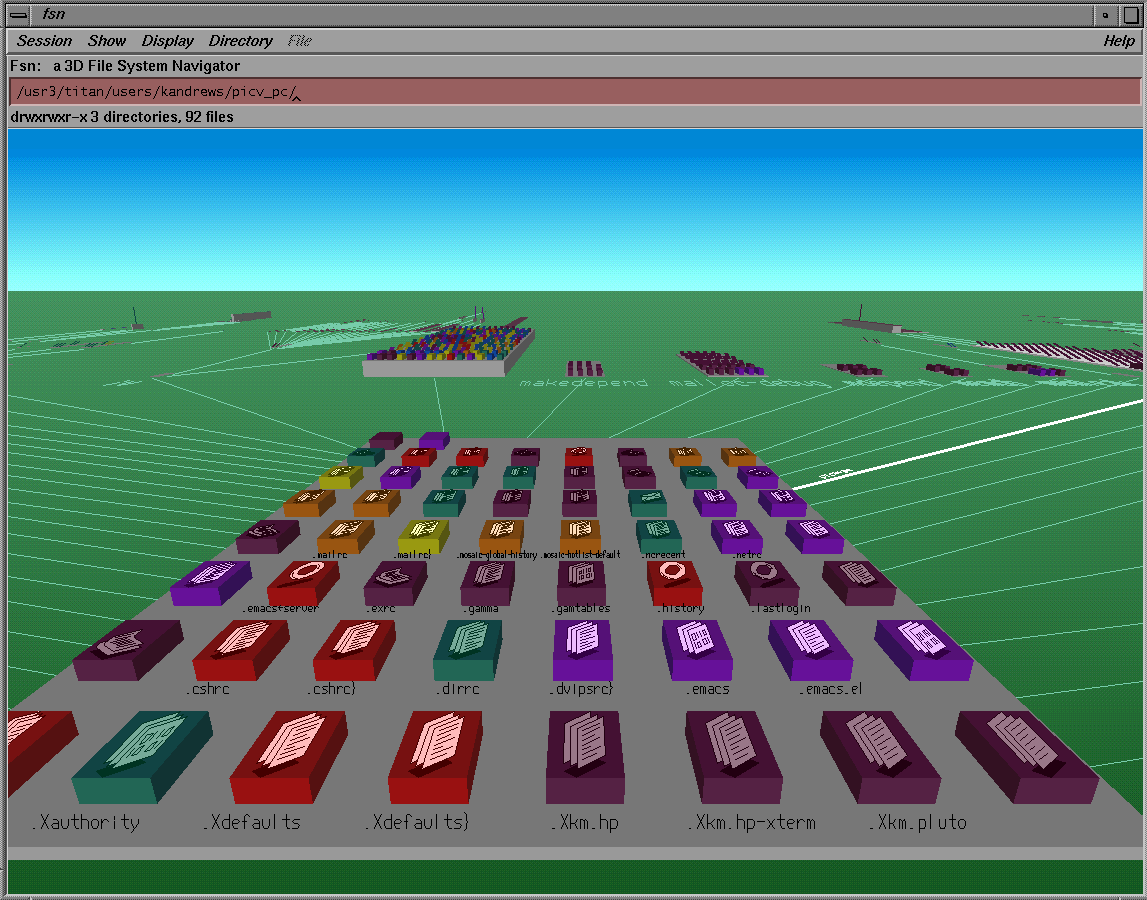
\includegraphics[width=8cm]{../grafik/fsn1.png}
\caption{FSN.}
\label{fig:fsn}
\end{figure}
\end{center}

\begin{center}
\begin{figure}[H]
    \centering
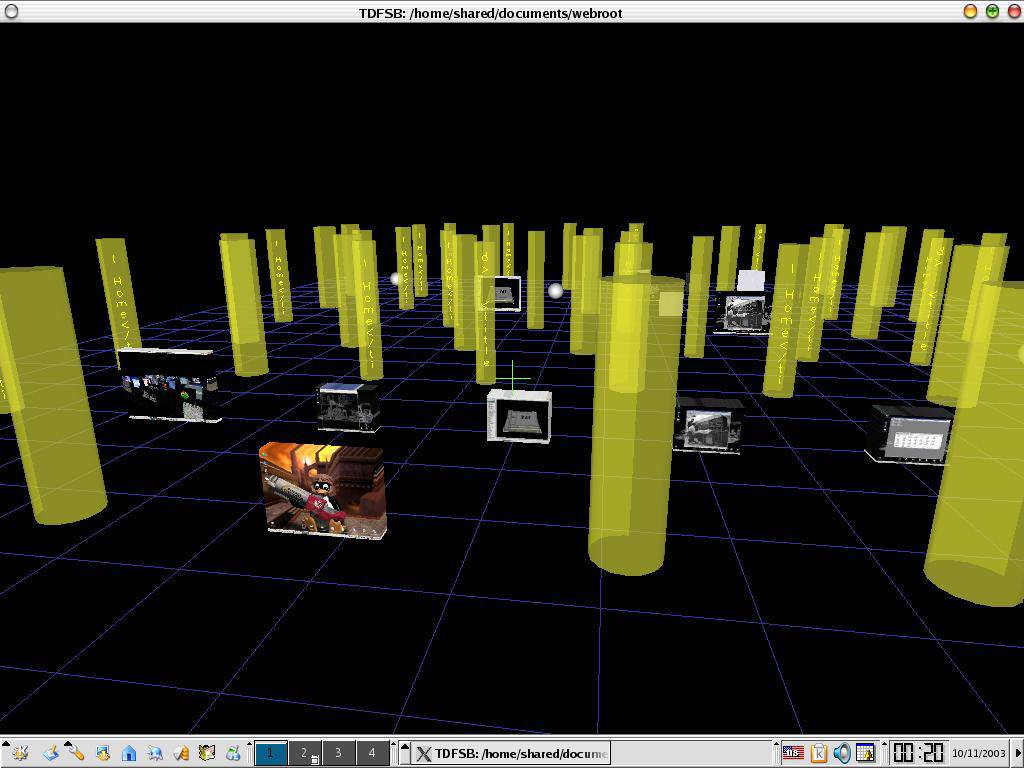
\includegraphics[width=8cm]{../grafik/tdfsb.jpg}
\caption{TDFSB.}
\label{fig:tdfsb}
\end{figure}
\end{center}

De ursprungliga obligatoriska kraven för produkten var följande:
\begin{LIPSkravlista}
\LIPSkrav{Original}{Alla filer ska representeras av block med någon textur på, är det en bild så ska bilden användas som textur}{1}

\LIPSkrav{Original}{Alla mappar ska representeras av block med någon textur}{1}
\LIPSkrav{Original}{Alla mappar och filer i en mapp ska vara placerade på en platta med en textur}{1}
\LIPSkrav{Original}{Ljussättningen ska ske med en Phong-shader}{1}
\LIPSkrav{Original}{Alla block ska ha skuggor}{1}
\LIPSkrav{Original}{Navigeringen ska vara first person där piltangenterna styr x och z koordinaterna och musen styr kameren i ett sfäriskt koordinatsystem}{1}
\LIPSkrav{Original}{Man ska inte kunna gå igenom filerna(collisions detection)}{1}
\LIPSkrav{Original}{Du ska kunna gå in i en mapp så transporteras du till den nya mappen)}{1}
\LIPSkrav{Original}{Du ska kunna klicka på en fil/mapp och få upp alla möjliga alternativ såsom radera, öppna...)}{1}
\LIPSkrav{Original}{Om du raderar en fil ska övriga filer ordna sig så det inte är några luckor någonstans}{1}
\LIPSkrav{Original}{Skydome ska finnas}{1}
\LIPSkrav{Original}{Endast Linux kommer stödjas}{1}
\end{LIPSkravlista}


och de ej obligatoriska kraven var följande:
\begin{LIPSkravlista}
\LIPSkrav{Original}{Du ska kunna få upp en terminal i filhanteraren}{2}
\LIPSkrav{Original}{Du ska kunna klicka på en mapp och sedan få upp en portal som du kan se in i mappen genom}{2}
\LIPSkrav{Original}{När du raderar en fil ska den explodera}{2}
\LIPSkrav{Original}{Innehåller en mapp många filer/mappar ska frustum culling användas för att minimera beräkningar}{2}
\LIPSkrav{Original}{Mapparnas texturer ska vara den ikon filen som operativsystemet använder med transparens, då ska renderingsordningen och vara korrekt}{2}
\end{LIPSkravlista}
Under projektets gång gick de obligatoriska kraven igenom en modifikation på grund av att projektet tog längre tid än vad jag trodde samt att en del inte riktigt passade in. Krav 5 togs bort på grund av tidsbrist, krav 6 gjordes om så att användaren bara navigerade i XZ planet då detta passade mycket bättre samt en del förenklingar kunde göras. Krav 9 togs bort då en terminal ansågs vara mycket enklare att implementera så all modifikation av filsystemet görs via den. Inga av de ej obligatorska kraven uppfylldes på grund av tidsbrist. I figur~\ref{fig:tmbtrf} kan man se resultatet. 
\begin{center}
\begin{figure}[H]
    \centering
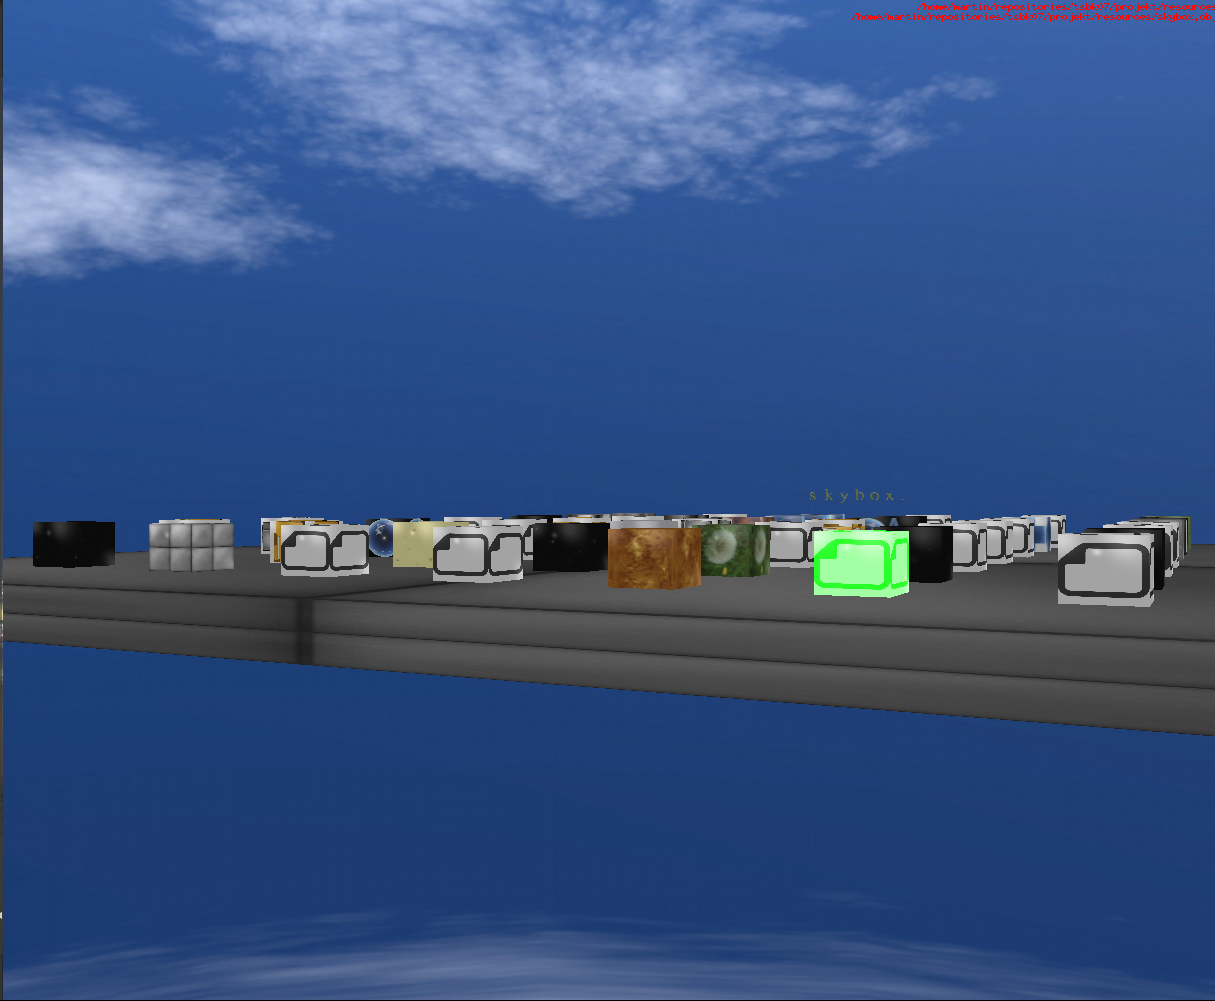
\includegraphics[width=8cm]{../grafik/tmbtrf.png}
\caption{TMBTRF.}
\label{fig:tmbtrf}
\end{figure}
\end{center}

\section{Bakgrund}
Det svåraste problemet jag hade innan jag började med projeketet var att på ett effektivt sätt interagera med datorns filsystem. Detta löstes rätt enkelt när jag upptäckte Boost::Filesystem. Detta bibliotek är inte speciellt använt så det finns inte så mycket hjälp att hitta på forum men dokumentation för det är väldigt bra så när jag väl kom in i det så fungera det väldigt bra. Funktioner såsom att byta namn och radera filer fanns redan implementerade så detta underlättade mycket.
\\
\\
Ett annat problem som var svårare än vad jag trodde var att visa filnamn i en 3D miljö. Den enklaste lösning skulle varit att använda något bibliotek för att generera texturer med en font till exempel FreeType. Jag försökte detta och jag kommer inte ihåg varför men jag fick det inte att fungera. För att få detta snyggt så skulle texturerna behöva vara transparenta så jag skulle behöva ta hänsynt till ordningen som alla objekt renderas. Min lösning på problemet var att generera .obj filer för alla tänkbara bokstäver och tecken som kan förekomma i ett filnamn. Jag valde alla bokstäver a-z och A-Z, alla siffror samt tecknen . - \_. Detta gjordes med ett python script i cad-programmet FreeCad. För att minimera inläsningstiden så läses alla dessa modeller in vid starten av programmet och återanvänds hela tiden. För att undvika problem som kan uppkomma vid långa filnamn som sträcker sig över hela miljön så visas bara de 7 första tecknen i filnamnet.
\\
\\
Anledningen till att C++ valdes var mest för dess datastrukturer såsom Vector, Map och string. Allting som kan göras i C++ kan självklart göras i C men där så är allting klart. Detta gjorde så att jag kunde göra en väldigt allmän klass som representerar alla objekt i 3D världen. Programmet arbetar också mycket med strängar och då är String väldigt mycket smidigare än en char array.
\\
\\
Ett problem som upptäcktes senare var att när man går in i en mapp som innehåller många filer, speciellt bilder, så tar det rätt lång tid innan hela världen har genererats. Detta skulle kunna lösas genom att ha en separat tråd som förbereder alla undermappar i den nuvarande mappen. Detta har dock inte implementeras men skulle jag fortsätta utveckla TMBTRF så skulle detta vara ett av de första problemen jag skulle lösa. 

\section{Teori}
I boken ''Software Product Quality Control'' \citep{SPQC} nämns ett antal definitioner som förtydligar vad kvalitetssäkring innebär, dessa syns nedan.  

\begin{itemize}
  \item ''Quality assurance: a planned and systematic pattern of all actions necessary to provide adequate confidence that an item or product conforms to established technical requirements.'' \citep[p.19]{SPQC} 
  \item ''Constructive quality assurance: All means to be used in constructing a product in a way so it meets its quality requirements.'' \citep[p.19]{SPQC} 
  \item ''Analyctical quality assurance: All means of analysing the state of the quality of a product.'' \citep[p.19]{SPQC} 
\end{itemize}
\noindent Kvalitetssäkring innebär följaktligen att man som leverantör av en produkt eller tjänst ska se till att de uppfyller de krav som har satts upp i en eventuell kravspecifikation. Det är dessa krav som sätter standarden för vad som är rätt nivå gällande kvalité. Under arbetsgången måste man analysera om man är på väg att uppfylla kraven eller inte, i sådana fall måste detta åtgärdas omedelbart.
\newline
\newline
Med detta sagt finns det flera steg i ett projekt att kvalitetssäkra. Ett effektivt sätt att göra detta på är genom att följa Shewhart cykeln, det vill säga planera, göra, studera och agera (PGSA) \citep{PDCA}. Shewhart cykeln är en iterativ fyra stegs metod, se figur \ref{fig:shewcycle}. Metoden är utvecklad av William Edwards Deming. Namnet ''Shewhart'' kommer från en av Demings kollegor \citep[p.~88]{Deming}. 
\begin{figure}[h]
\centerline{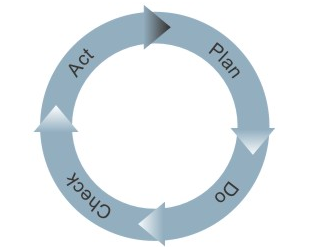
\includegraphics[scale=0.5]{ruben-tex/graphic/shewhartcycle}}
\caption{Shewhart cykeln \citep{Mindtools}}
\label{fig:shewcycle}
\end{figure}
\begin{enumerate}
  \item Planera. I detta skede ska målet fastställas, det vill säga sätta upp de krav som behövs för att kunden skall bli nöjd. Genom att göra detta är det tydligt om vad som skall göras och en överenskommelse finns mellan kund och leverantör. 
  \item Göra. När man konstaterat vad som behöver göras för att kunden skall bli nöjd är det dags att implementera ett sätt att arbeta och fullfölja processen.
  \item Studera. Efter att ha följt processen under en viss period är det dags att utvärdera om processen man har följt kommer leda till att man uppfyller de målen man har fastställt i planeringsfasen.
  \item Agera. Om man under studeringsfasen upptäcker att processen man följer inte kommer leda till att man uppfyller de krav som kund och leverantör var överens om måste detta åtgärdas omedelbart genom att planera om arbetsprocessen eller i viss mån diskutera kraven med kunden. Om processen som följs kommer uppfylla de krav som har satts upp kan man fortsätta med iterationerna av Shewhart cykeln precis som innan.
\end{enumerate}
\begin{figure}[h]
\centerline{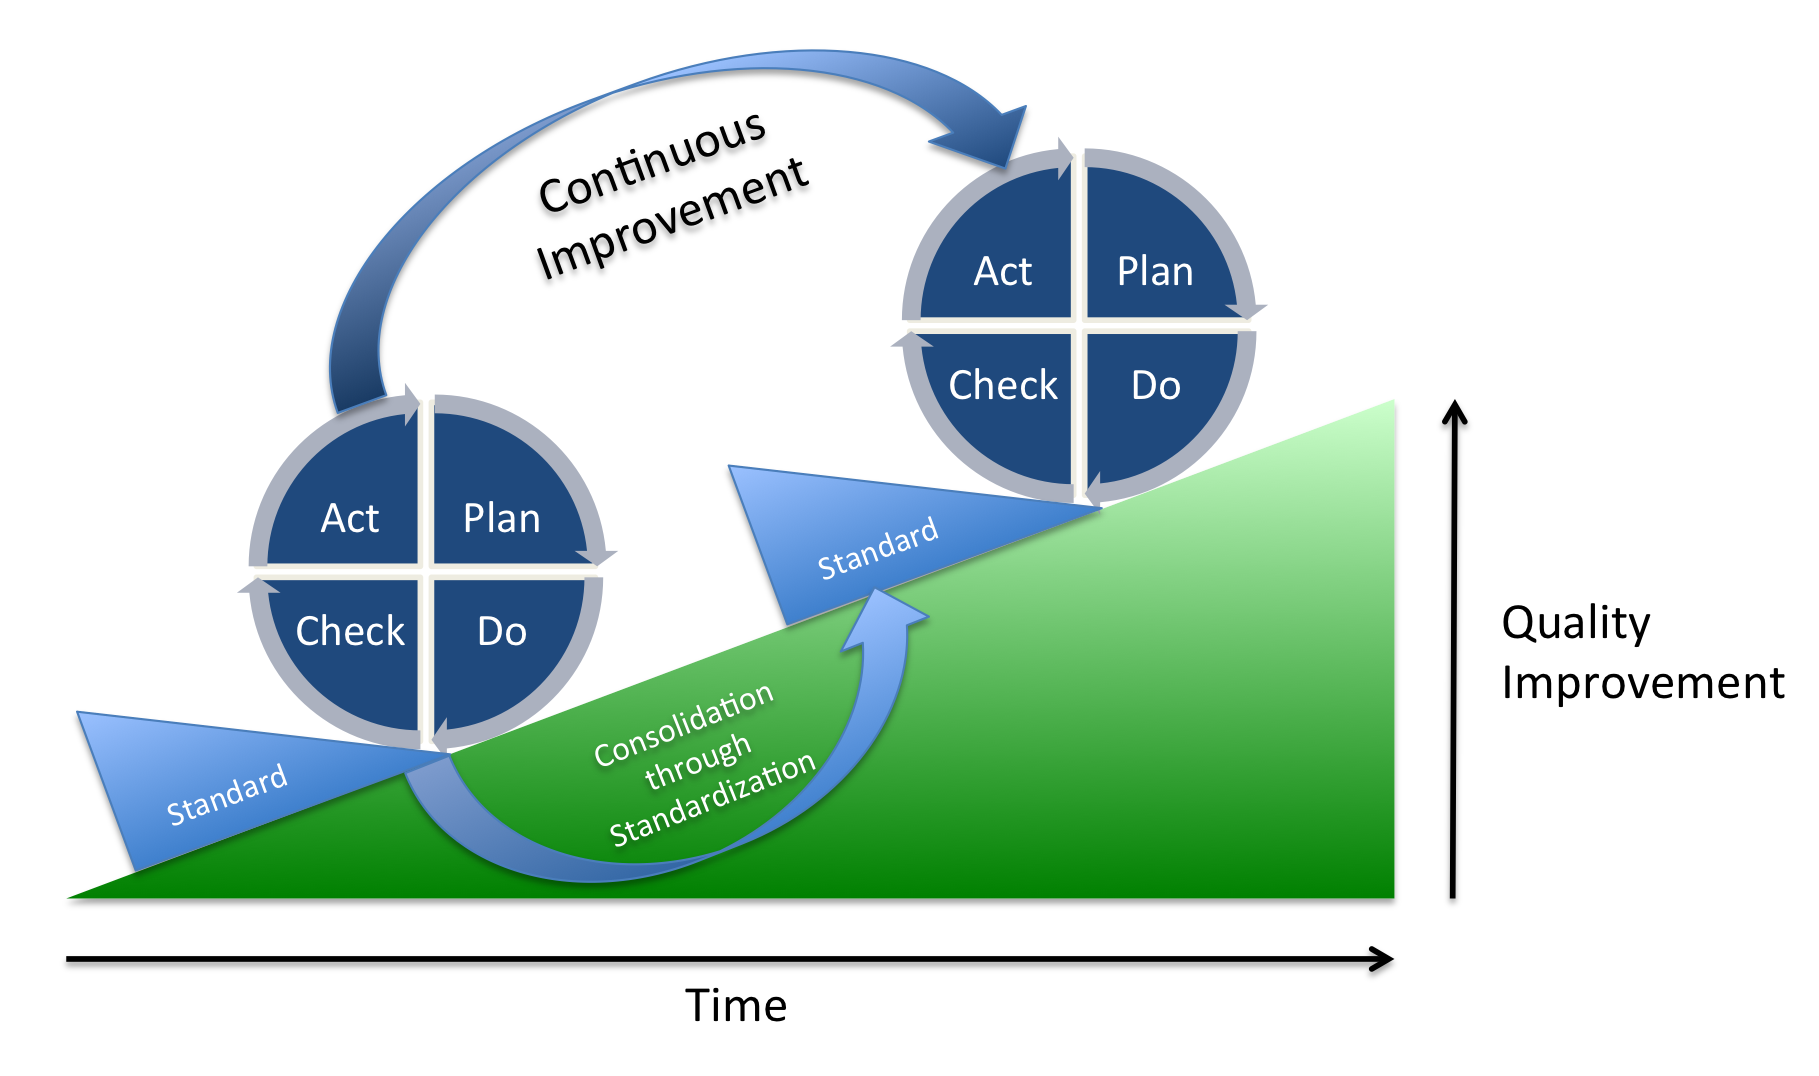
\includegraphics[scale=0.15]{ruben-tex/graphic/PDCA_Process}}
\caption{PDCA process \citep{Vietze}}
\label{fig:pdcaprocess}
\end{figure}
\noindent Genom att följa Shewhart cykeln under ett projekt kan man iterativt förbättra sin arbetsprocess och genom detta öka kvaliteten av den produkt man utvecklar, se figur \ref{fig:pdcaprocess}.
\newline
\newline
När det väl är dags för överlämning av en produkt eller tjänst är det bra att göra en kravinspektion innan. En kravinspektion enligt IEEE standarden för ''Software reviews'' syns nedan.

\begin{tcolorbox}[boxrule=1pt,leftrule=5pt,arc=0pt,auto outer arc]
\textbf{''}A process or meeting during which a software product is examined by a project personnel, managers, users, customers, user representatives, or other interested parties for comment or approval\textbf{''} \citep{SFSR}
\end{tcolorbox}

\noindent
Det man vill få gjort med en kravinspektion är alltså att produkten eller tjänsten som har tagits fram ska utvärderas av berörda parter så att den uppfyller de krav som har fastställts i ett tidigare skede för ett godkännande. En kravinspektion kan se ut som sådan \citep{Sandahl}:
\begin{enumerate}
\item{Tillträde.}
\item{Planering och översikt. Under detta steg sker en planering över hur inspektionen ska gå till och en översikt av produkten ges.}
\item{Individuell granskning. De berörda parterna granskar produkten eller tjänsten.}
\item{Möte. Efter granskningen görs en lista av alla de defekter som kan ha hittats.}
\item{Ändringar och uppföljning. I detta skede åtgärdar man de defekter som stöttes på och normalt brukar verifiera detta.}
\item{Utträde.}
\end{enumerate}

\subsection{Sammanfattning}
Sammanfattningsvis kan man konstatera att ett återkommande tema för att ta fram en högkvalitativ produkt eller tjänst är att planera, utföra och granska, för att sedan upprepa proceduren under projektets gång. Detta är dock bara en teoretisk tillämpning och verkligheten kan se annorlunda ut.

\section{Metod}
	För att ta reda på all information som behövs har ett flertal böcker blickats igenom. Ingen av dem har läst till 100\%, utan endast de intressanta delarna har läst med mer nogrannhet. För att verifiera att det som lästs stämmer har vissa delar testats i praktiken, i detta fall på projketet. Till exempel så har enhetstester körts på matris bibliotekts funktioner såsom matrisaddition, sytemtester och modultester har körts på den kvadratiska problem-lösaren och acceptanstester har körts på alla delar i projektet för att se till att alla krav är uppfyllda. Mer om detta kan läsas i resultat.
	
\subsection{Enhetstest}
	I ''Software Unit Testing'' \citep{ivv} definierar ett enhetstest som ett test på den minsta möjliga samlingen kod som fortfarande går att testa nyttofullt, alltså att koden är tillräckligt stor för att fel ska kunna uppstå. Dessa test är bra då de är riktade mot en så liten portion med kod och i och med detta sällan missar buggar och fel. Det som kan vara krångligt med enhetstest är att just hitta dessa minsta samlingarna med kod, speciellt om det är en extern part (en annan programmerare) som ska skapa och utföra testen. I och med att man kör enhetstester på så små delar av kod har de i teorin en tendens till att bli väldigt många om man ska täcka tillräckligt stor funktionalitet. Detta är dock oftast inget problem i praktiken eftersom många små funktioner ofta är triviala och har ytterst få uppgifter. Då behöver inte så många test skrivas, om ens ett enda.
\subsection{Modultest}	
	Det finns flera olika definitioner av vad en modul är, och i och med det blir det då svårt att definiera vad ett modultest är. I ''The Art of Software Testing'' definierar de att moduler och enheter är samma sak men jag har valt att istället gå efter Kristian Sandahls definiton. Han definierar att ett modultest är ett integrationtest utav två eller fler enheter. Det går ut på att man kombinerar ett antal enheter och sedan testar dem tillsammans. Testen i sig kan var väldigt lika enhetstest men täcker nu en mer komplex funktionalitet. Precis som enheter kan moduler vara svåra att definiera. Om allt för många enheter förs samman och modulen får mer funktionalitet kanske den till slut kan klassas som ett system, och då förlorar modultestningen sitt syfte. Om man har ett så litet projekt som detta så är moduldefinitionen ofta inte så svår, eftersom både komplexiteten och utvecklingsmöjligheterna är begränsade. Det är kritiskt vid dessa test att underliggande funktioner redan är testade. Om inte, kan i stort sett inga slutsatser, angående vad som är fel, dras när ett test misslyckas.
\subsection{Systemtest}	
	Ett systemtest är precis som modultest ett integrationstest, men nu utav ett antal moduler istället. Enligt ''The Art of Software Testing'' inriktar sig testet nu också vanligtvis på hela produkten som har utvecklats, för att se om funktionalitetskraven är uppfyllda. Detta för att säkerställa dess funktionalitet och för att hitta fel som uppstått vid kommunikation mellan moduler. Exempel på systemtest i vårt projekt är test av lösaren. Anledningen till att lösaren ses som ett eget system och inte är ihopbakad med GUI:t är att den ska kunna fungera separat. Givetvis är de båda ihopbakade också ett system, som också kräver systemtest.	
\subsection{Acceptanstest}	
	Ett acceptanstest är ett test som har målet att testa om programmet är acceptabelt. Med det menas att testen validerar ifall programmet uppfyller alla krav som ställs på det, och nu inte endast funktionalitetskraven. I vårt projekt är det huvudsakligen prestandan som behöver acceptanstestas. Då det prestandakrav produkten hade var relativt vagt ("Produkten ska ha likvärdig prestanda med Gurobi"), och att kravet sedan förhandlades bort, gjorde att testen inte hade så stor prioritet. Men för att få någon vetskap om produktens hastighet och för att garantera att kunden blir nöjd krävs ändå någon form utav test.
\subsection{Övrigt}	
	I projektet har även ett byggsystem använts, som smidigt kompilerat all kod automatiskt. Systemet har därefter även kört alla tester som skapats genom projektet.
	Med hjälp av byggsystemet och Kontinuerlig Integration har all kod då kunnat testas direkt när någon har skrivit ny kod och därav har det gått att se när och var feluppstått. Och eftersom systemet även har kört alla gamla test har koden säkerställts med att alla andra funktioner, de som inte har rörts, också fortfarande fungerar.
\section{Resultat}	
	Följande del beskriver hur arbetet med efterforskningen gick samt hur testen utfördes.
	\subsection{Efterforskning}
	Det finns otroligt mycket information om mjukvarutestning men samtidigt är ämnet ganska vagt då testning beror så mycket på just vad som ska testas. I vårt projekt visade det sig att ''Black Box''-testning var den metod som överlägset lämpade sig bäst. ''Black Box'' går ut på att man sätter en ''svart låda'' över det som ska testas, så att man endast kan se in- och utdatan. Sedan tittar man på utdata och ser ifall den är den förväntade. ''Black Box'' anses bra i detta projekt eftersom hela Quadopt är uppbyggd utav många små funktioner och resultateten som de ska ge tillbaka är oftast kända på förhand. Ett exempel på detta är matrisaritmetiken där resultatet, av till exempel en multiplikation, går att räkna ut ganska enkelt på papper. Enligt ''The Art of Software Testing'' ska dessa test utgå ifrån kravspecifikationen och andra dokument som beskriver vad produkten ska ha för funktionalitet. Boken beskriver också ''Black Box'' som en utmattande testteknik. Med det menar de att man borde testa alla möjliga indata till den svarta lådan och se så att svaren stämmer. Detta är precis som det står i boken i praktiken omöjligt. Speciellt i vårt projekt där det enda som begränsar antalet olika sätt en matris, bestående utav tal, kan se ut på är datorns minne. \newline
I projektet fanns dock ofta behovet av se en funktions lösningsgång, och då är ''Black Box'' en väldigt dålig metod. En metod som då lämpar sig bättre är ''White Box'' testning, som innebär att man tittar på den interna strukturen i en funktion. Därefter kan man se, efter vald indata, om lösningsgången är den väntade. I ''The Art of Software Testing'' står det att även denna metod kan problematisk då antalet lösningsgångar kan vara väldigt många. För att se om det ens är rimligt att utföra dessa test kan man se på funktionens cyklomatiska komplexitet. Cyklomatisk komplexitet innebär att man gör en graf över funktionen där de möjliga stadierna i lösningsgången är noder, och de möjliga lösningsvägarna är bågar. I ''Structured testing'' \citep{structest} står det att om denna komplexitet är för stor ökar antalet fel som programmeraren gjort väldigt fort, och samtidigt blir det i stort sett omöjligt att utföra några ''White Box''-test då fel kan uppstå på så många ställen. \\ 	
För att säkerställa projektets krav behövdes bara en testmetod till, och det var en metod för att mäta prestanda. Den som valdes var ''Load testing'' som innebär att man belastar programmet med mycket data och ser hur bra det fungerar. I projektets fall gavs lösaren många problem och tittade på hur fort det gick i förhållande till andra lösare. \newline	
Det skulle kunnat varit så att GUI:t hade haft högre prioritet än vad det hade. I det fallet hade olika typer av UX- och användartest varit nödvändiga för att kvalitetssäkra produkten. Men eftersom GUI:t beställdes utifrån kundens personliga behov, var det tydligt definierat redan från början att det var av låg prioritet. 
	
	\subsection{Praktik}
	Som beskrivet tidigare finns det i stort sett oändligt många kombinationer av in- och utdata.	För att då kunna utföra ''Black Box''-testerna behövdes antalet testfall reduceras. Detta åstadkoms genom att ha möten med kunden som klargjorde att indata till programmet alltid skulle vara giltig. Det reducerade antal testfall enormt mycket, men som beskrivet i resultatet av efterforskningen finns det även väldigt mycket giltig indata. Exempelvis för matrisaritmetiken. Dessa test gick också att reducera genom att de flesta operationer är triviala och endast kräver numeriska test såsom nolldivision och flyttalsfel. Genom att även utnyttja ''White Box''-tekniken gick det att utforma olika ''Black Box''-test som tog olika vägar genom koden och på så sätt bara skapa ett test för varje väg. Denna teknik utnyttjades endast på mindre funktioner såsom moduler för att antalet olika fall skulle begränsas till något som var rimligt. \newline
	För lösaren gick det att applicera samma metod, eftersom dess funktionalitet bygger mycket på underliggande funktioner. Det som skilde sig gentemot småfunktionerna var att nu behandlades oftast rader eller kolumner i matriser istället för enskilda element. Detta ledde till att de flesta test kontrollerade på kanterna utav det tillåtna området. Alltså kunde ett test vara att försöka hämta ut en radvektor på rad -1 ur en matris, vilket skulle vara ogiltigt.\newline
Vid granskning av testresultat från Git, Travis (verktyg för Kontinuerlig integration) och gruppmedlemmar visade det sig att majoriteten fel av bestod utav två typer: ''Assertion''s som misslyckats och ''Segmentation fault''. En ''Assertion'' är ett test inuti koden som avbryter exekveringen om testet inte går bra. ''Segmentation fault'' är ett programmeringsfel som resulterat i en ogiltig läsning eller skrivning till minnet. Felen som uppstod var väldigt utspridda och olika. Det som de flesta hade gemensamt var dock att de låg på en låg nivå, alltså i bottenfunktionerna. \newline	
	För att testa algoritmens hastighet stötte gruppen på oväntade problem, lösarna var för snabba.	Då varje testkörning tog 0.00 sekunder för alla lösarna förutom MATLAB behövdes testen köras många gånger för att se en tydlig skillnad. Anledningen till att MATLAB är långsammare är för att den är oerhört generell men förmodligen inte gjorts med fokus på att vara snabb. Gurobi är snabb eftersom dess enda uppgift är att lösa sådana här problem och har arbetats på under lång tid. Vår algoritm är snabb eftersom den inte är generell, alltså bryr vi oss inte om vissa specialfall som vi aldrig kommer stöta på. \newline
	För att då testa deras prestanda fick lösarna lösa olika optimeringsproblem många gånger, ofta upp emot 1000 gånger, för att kunna skilja deras egentliga hastighet. Att köra testen på vår lösare och i MATLAB var enkelt då vi hade funktionalitet för att konvertera matriser från MATLABs definition till vår, och vice versa. Däremot så var det krångligare i gurobi eftersom tiden som var allokerad för utbildning av programmet var begränsad. Det tvingade gruppen till att mata in problemet på ekvationsform vilket gjorde att gruppmedlemmarna var tvungna att köra endast små tester. Redan vid problem med fler än 10 bivillkor skulle det ta väldigt lång tid att konvertera och mata in problemet. \newline
	
	
	\subsection{Enhetstester}
	Under projektet har många enhetstest skrivits (framförallt för matrisbiblioteket). Dessa test har skrivits innan och under kodningen och sedan utförts direkt efter att koden blivit klar. Det som var intressant med dessa test var mängden av fel som upptäcktes direkt. Det ledde till att utvecklingen blev mycket effektiv då fel kunde åtgärdas direkt.
	
	\subsection{Integrationstester}
	De modultester som planerades och utfördes under projektet var framförallt lösarens funktioner. Modulerna var uppbyggda utav sammansättningar av enheter från matrisbiblioteket och andra strukturer. Dessa test utfördes vanligtvis samtidigt som implementeringen pågick. Detta för att hela tiden se till att rätt protokoll och gränssnitt användes.\\
De systemtester som utförts är tester utav lösaren och subproblemslösaren. Dessa ansågs vara tillräcklig komplexa för att ses som system. 
	
	
	\subsection{Acceptanstester}
	De acceptanstester som utförts under projektet är framförallt prestandatester. Detta då det enda kravet lösaren hade var att den skulle vara ungefär lika snabb som den kommersiella lösaren Gurobi. Då detta krav sedan togs bort lade mindre energi på prestandatester. Men de delar som ändå testats var framförallt underfunktioner till lösaren, såsom matrisbiblioteket och subproblemslösaren.
	
	\subsection{Misstag}
	Det hände att vissa modul- och systemtester skedde innan de underliggande enheterna blivit testade. Ett exempel på det är lösaren, som gruppen ivrigt ville få igång och började därför testa den tidigt. Då den inte fungerade korrekt gjorde detta att det tog lång tid att hitta felen som förmodligen hade upptäckts mycket snabbare om bara rätt testprocess hade använts.
	
	
\section{Diskussion}
Under denna del kommer en diskussion angående om resultaten ske samt metoderna som användes.
\subsection{Resultat}
Resultaten för alla tre punkter måste anses vara rimliga. Den första punkten angående vad som är rätt nivå är en väldigt diffus fråga och kan bara svaras genom att båda parter, dvs leverantör och kund har ett enhetligt svar. Eftersom det man kommer överens om i en eventuell kravspecifikation måste räcka att fullfölja för att det ska klassas som rätt nivå gällande kvalité. Sen om kunden hade velat haft några andra funktioner med produkten eller tjänsten så borde kunden ha specificerat detta. Leverantörer har också skyldighet att försöka uppfylla alla krav som har specificerats på ett snyggt sätt och inte bara slänga ihop något som fungerar, små detaljer kan utmärka ett arbete.
\newline
\newline
Den andra punkten finns det inte mycket att diskutera om, som allt annat i livet krävs det struktur för att man ska uppnå något. Under teoridelen i kapitel tre kan man konstatera att planera, utföra och granska antagligen kommer generera en produkt eller tjänst av tillräckligt god kvalité.
\newline
\newline
Angående den sista punkten kan man byta svaret från ett ja till ett nej, då ett krav förhandlades bort. I detta projekt hade kandidatgruppen endast ett mätbart krav, detta krav specificerade att optimeringsalgoritmen skulle vara likvärdig i hastighet i jämförelse med en kommersiell mjukvara kallad ''Gurobi''. ''Gurobi'' specialiserar sig i att lösa olika sorters optimeringsproblem \citep{gurobi}. Under projektets slutskede diskuterade kandidatgruppen med kunden om att det kommer bli svårt att vara jämbördig med ''Gurboi'', detta var inget problem för kunden och kravet kunde tas bort. Kunden tryckte på att det viktigaste var att koden fungerar och att den är väldokumenterad, vilket den är. Däremot kan jag tycka att om man tar bort ett krav så har man misslyckats och därför anser jag att man kan ändra svaret till nej, slutprodukten håller inte tillräckligt god kvalité, men då är jag väldigt hård mot mig själv och kandidatgruppen. Däremot säger teorin bakom det hela att produkten håller tillräckligt god nivå då den uppfyller alla krav, det ska inte spela någon roll om man har förhandlat bort något krav eller inte.

\subsection{Metod}
Efter slutförandet av projektet och analys av hur det hela gick finns det många saker man hade kunnat gjort annorlunda. Ett återkommande problem som stöttes på under projektets gång var att kodstandarden som hade satts upp från början inte följdes helt och hållet, inte förens den sista iterationen skrevs kod efter den. Detta resulterade i att mycket tid lades ner på att refaktorera kod. Kodstandarden innehöll inte heller allt som bör ta hänsyns till. Ett exempel är att frigöra minne, vilket resultera i att mycket tid lades ner på att hitta och åtgärda minnesläckor. Eftersom kandidatgruppen hade ett krav på att skriva pålitlig kod så är förstås minnesläckor inte accepterbart. 
\newline
\newline
Jag tror att slutprodukten skulle ha sett annorlunda ut om kodstandarden täckte fler områden i hur man ska skriva kod samt om man tryckte på hur viktigt det är att följa kodstandarden. Jag som kvalitetsamordnare hade kunnat trycka mer på att kodstandarden skall följas för att en produkt av bättre kvalité skulle skapats.
\newline
\newline
I teoridelen visade forskningen att om man ska uppnå en högkvalitativ produkt kan man t.ex. använda sig av Shewhart cykeln, planera, göra, studera och agera. Kandidatgruppen planera hur man skulle skriva kod, man följde inte kodstandarden, kandidatgruppen var väl medveten om det. Vid detta stadiet borde man agera, visserligen sas det åt folk att börja använda kodstandarden, men det hade nog varit bättre att utvärdera om kodstandarden och föra dialog om varför den inte följs för att skriva en ny som möjligtvis alla känner sig bekväma med.

\section{Slutsatser}
{\LaTeX} lämpar sig mycket väl för teknisk dokumentation i ett programmeringsprojekt. Denna slutsats kan dras från det {\LaTeX} dokument gruppen har producerat. {\LaTeX} gav oss verktygen för att infoga figurer, matematiska formler, ekvationer, algoritmer och pseudokod som behövdes för dokumenten i projektet.   
\newline
\newline
Det tog hela projekttiden för att samtliga medlemmar skulle känna att de behärskade {\LaTeX}. Detta kan ses som en lång inlärningskurva för språket och att det tog onödig tid från andra delar av projektet. Dock var detta aldrig egentligen något problem, mycket hjälp fanns att hämta från internet och då två av gruppmedlemmarna behärskade {\LaTeX} sedan tidigare kunde de hjälpa och lära resten av gruppen. 
\newline
\newline
Om ingen av gruppens medlemmar hade använt {\LaTeX} sedan tidigare kan det diskuteras om det hade varit lönsamt för gruppen att lära sig det. Då hade mer tid behövts läggas på utbildning av språket och andra uppgifter hade fått lida. Som sagt lämpar sig {\LaTeX} mycket väl för teknisk dokumentation i ett programmeringsprojekt och även om det hade tagit mer tid så hade det varit värt i det långa loppet.    


\newpage

%Rubens report
\stopcontents[sections]
\resumecontents[default]
\addcontentsline{toc}{section}{\protect\numberline{G} Kvalitetssäkring}
\stopcontents
\startcontents[sections]
\LIPSTitelsidaruben
\setcounter{section}{0} 
\printcontents[sections]{ }{1}{}
\newpage
\section{Inledning}
Jag har gjort en filhanterar som visualiserar alla filer och mappar i 3D med hjälp av OpenGL. Inspirationen till detta projekt var bland annat FSN (File System Navigator) som gjordes av SGI för IRIX systemen och FSV(File System Visualizer) som är en remake av FSN på Linux, se figur~\ref{fig:fsn}. En annan inspiration var det lite modernare TDFSB som även visar upp bilder och filmer i 3D världen, se figur~\ref{fig:tdfsb}. 

\begin{center}
\begin{figure}[H]
    \centering
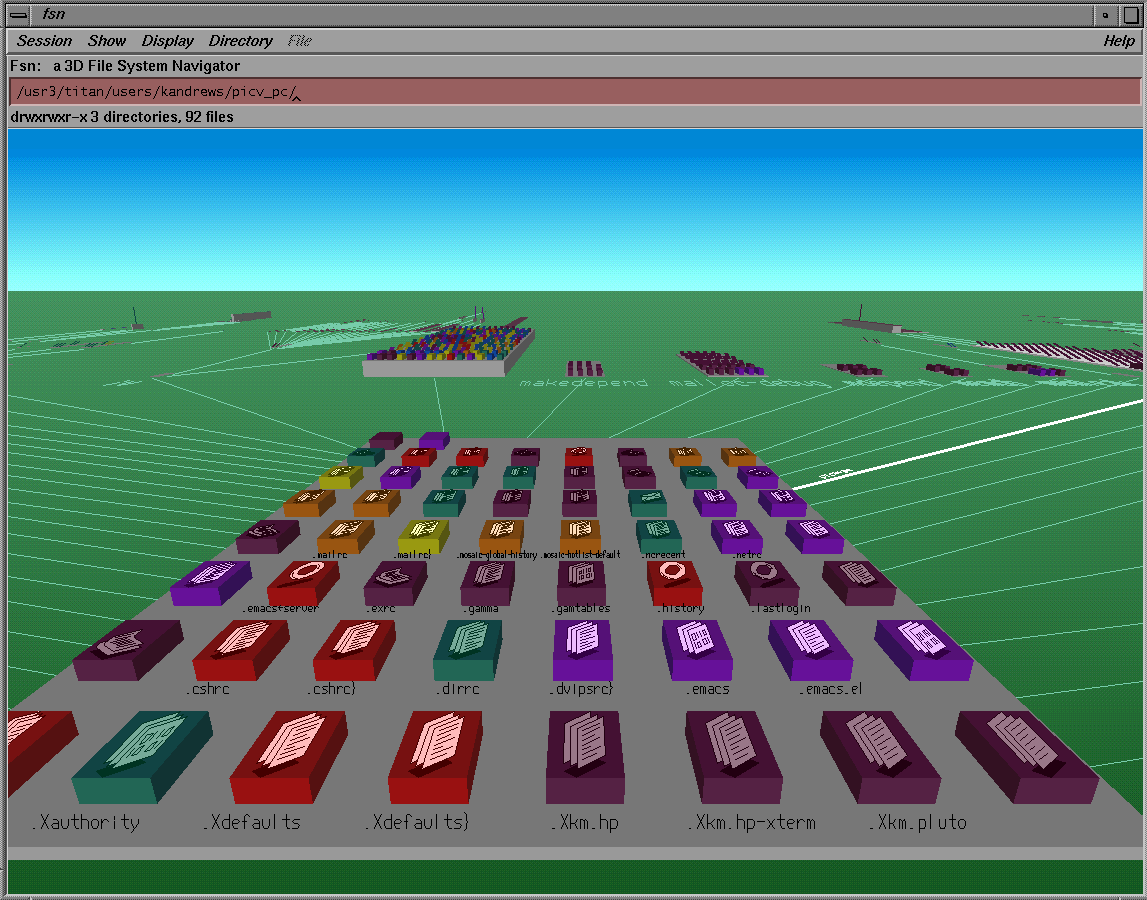
\includegraphics[width=8cm]{../grafik/fsn1.png}
\caption{FSN.}
\label{fig:fsn}
\end{figure}
\end{center}

\begin{center}
\begin{figure}[H]
    \centering
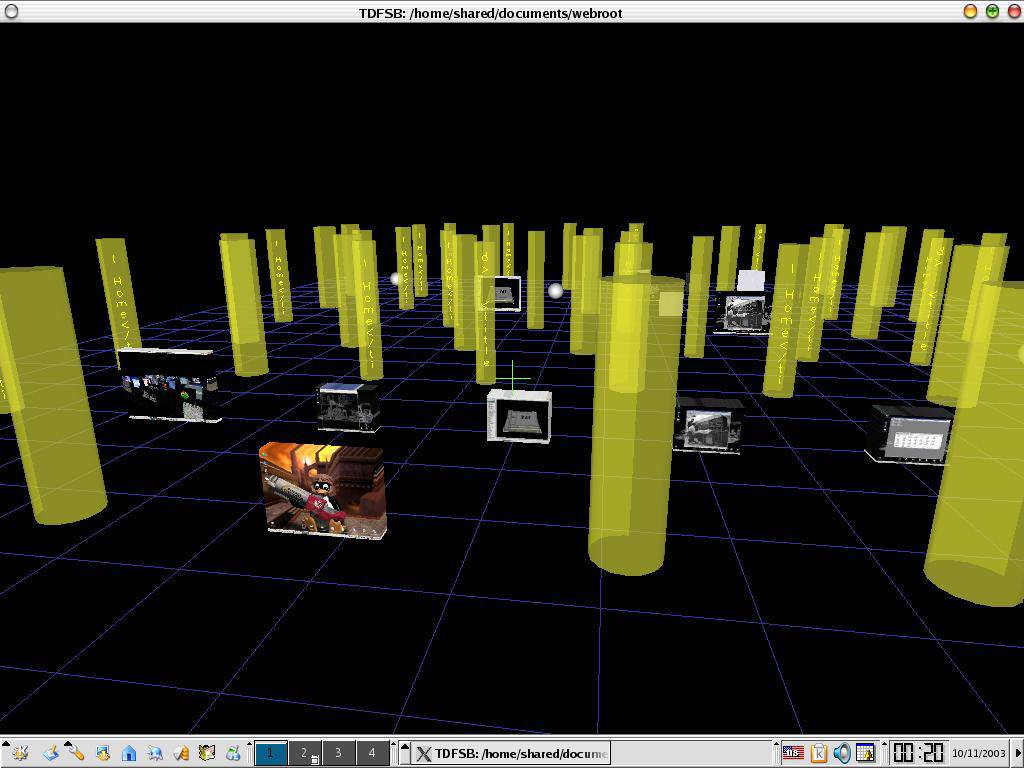
\includegraphics[width=8cm]{../grafik/tdfsb.jpg}
\caption{TDFSB.}
\label{fig:tdfsb}
\end{figure}
\end{center}

De ursprungliga obligatoriska kraven för produkten var följande:
\begin{LIPSkravlista}
\LIPSkrav{Original}{Alla filer ska representeras av block med någon textur på, är det en bild så ska bilden användas som textur}{1}

\LIPSkrav{Original}{Alla mappar ska representeras av block med någon textur}{1}
\LIPSkrav{Original}{Alla mappar och filer i en mapp ska vara placerade på en platta med en textur}{1}
\LIPSkrav{Original}{Ljussättningen ska ske med en Phong-shader}{1}
\LIPSkrav{Original}{Alla block ska ha skuggor}{1}
\LIPSkrav{Original}{Navigeringen ska vara first person där piltangenterna styr x och z koordinaterna och musen styr kameren i ett sfäriskt koordinatsystem}{1}
\LIPSkrav{Original}{Man ska inte kunna gå igenom filerna(collisions detection)}{1}
\LIPSkrav{Original}{Du ska kunna gå in i en mapp så transporteras du till den nya mappen)}{1}
\LIPSkrav{Original}{Du ska kunna klicka på en fil/mapp och få upp alla möjliga alternativ såsom radera, öppna...)}{1}
\LIPSkrav{Original}{Om du raderar en fil ska övriga filer ordna sig så det inte är några luckor någonstans}{1}
\LIPSkrav{Original}{Skydome ska finnas}{1}
\LIPSkrav{Original}{Endast Linux kommer stödjas}{1}
\end{LIPSkravlista}


och de ej obligatoriska kraven var följande:
\begin{LIPSkravlista}
\LIPSkrav{Original}{Du ska kunna få upp en terminal i filhanteraren}{2}
\LIPSkrav{Original}{Du ska kunna klicka på en mapp och sedan få upp en portal som du kan se in i mappen genom}{2}
\LIPSkrav{Original}{När du raderar en fil ska den explodera}{2}
\LIPSkrav{Original}{Innehåller en mapp många filer/mappar ska frustum culling användas för att minimera beräkningar}{2}
\LIPSkrav{Original}{Mapparnas texturer ska vara den ikon filen som operativsystemet använder med transparens, då ska renderingsordningen och vara korrekt}{2}
\end{LIPSkravlista}
Under projektets gång gick de obligatoriska kraven igenom en modifikation på grund av att projektet tog längre tid än vad jag trodde samt att en del inte riktigt passade in. Krav 5 togs bort på grund av tidsbrist, krav 6 gjordes om så att användaren bara navigerade i XZ planet då detta passade mycket bättre samt en del förenklingar kunde göras. Krav 9 togs bort då en terminal ansågs vara mycket enklare att implementera så all modifikation av filsystemet görs via den. Inga av de ej obligatorska kraven uppfylldes på grund av tidsbrist. I figur~\ref{fig:tmbtrf} kan man se resultatet. 
\begin{center}
\begin{figure}[H]
    \centering
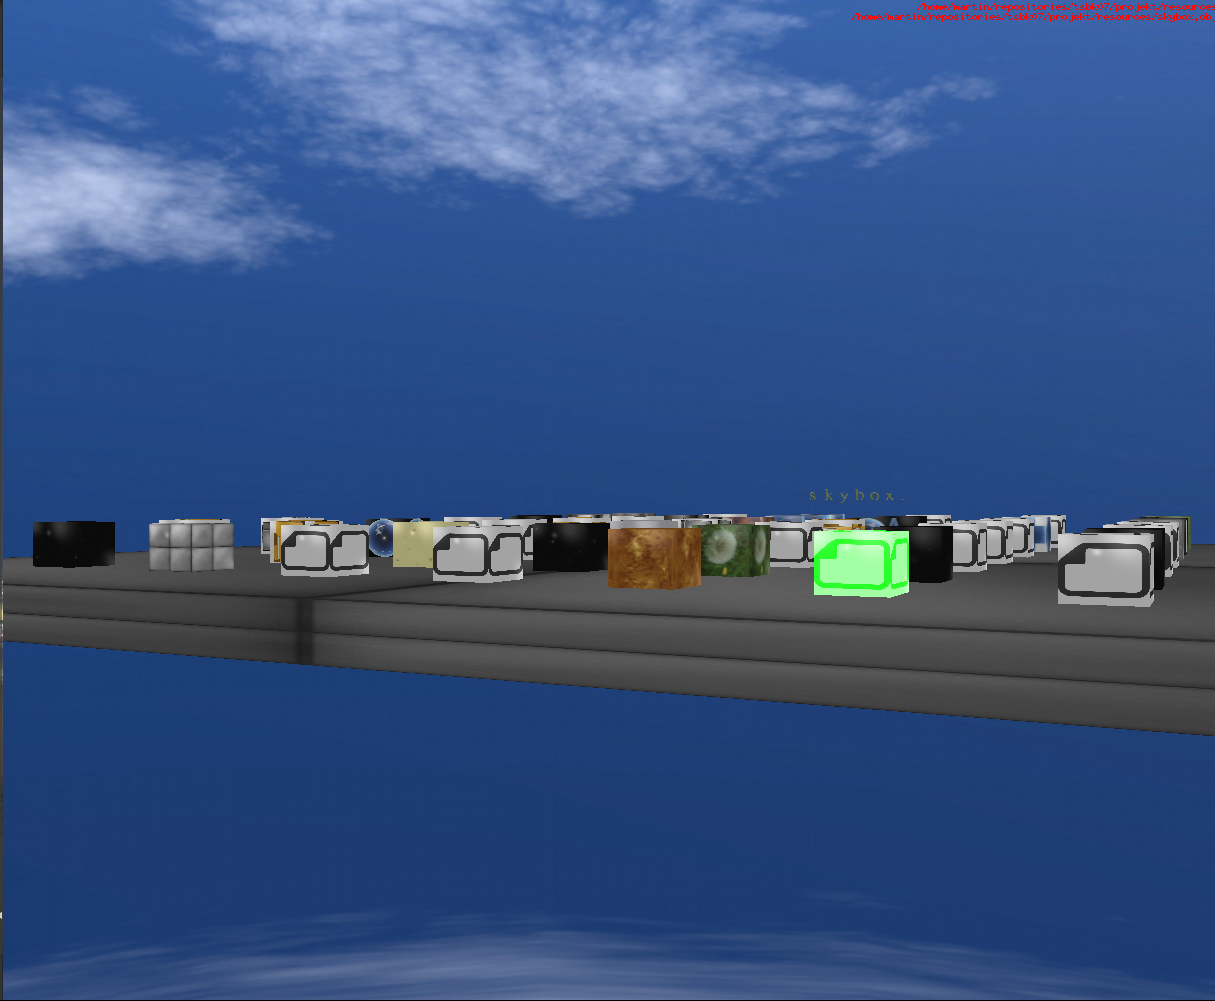
\includegraphics[width=8cm]{../grafik/tmbtrf.png}
\caption{TMBTRF.}
\label{fig:tmbtrf}
\end{figure}
\end{center}

\section{Bakgrund}
Det svåraste problemet jag hade innan jag började med projeketet var att på ett effektivt sätt interagera med datorns filsystem. Detta löstes rätt enkelt när jag upptäckte Boost::Filesystem. Detta bibliotek är inte speciellt använt så det finns inte så mycket hjälp att hitta på forum men dokumentation för det är väldigt bra så när jag väl kom in i det så fungera det väldigt bra. Funktioner såsom att byta namn och radera filer fanns redan implementerade så detta underlättade mycket.
\\
\\
Ett annat problem som var svårare än vad jag trodde var att visa filnamn i en 3D miljö. Den enklaste lösning skulle varit att använda något bibliotek för att generera texturer med en font till exempel FreeType. Jag försökte detta och jag kommer inte ihåg varför men jag fick det inte att fungera. För att få detta snyggt så skulle texturerna behöva vara transparenta så jag skulle behöva ta hänsynt till ordningen som alla objekt renderas. Min lösning på problemet var att generera .obj filer för alla tänkbara bokstäver och tecken som kan förekomma i ett filnamn. Jag valde alla bokstäver a-z och A-Z, alla siffror samt tecknen . - \_. Detta gjordes med ett python script i cad-programmet FreeCad. För att minimera inläsningstiden så läses alla dessa modeller in vid starten av programmet och återanvänds hela tiden. För att undvika problem som kan uppkomma vid långa filnamn som sträcker sig över hela miljön så visas bara de 7 första tecknen i filnamnet.
\\
\\
Anledningen till att C++ valdes var mest för dess datastrukturer såsom Vector, Map och string. Allting som kan göras i C++ kan självklart göras i C men där så är allting klart. Detta gjorde så att jag kunde göra en väldigt allmän klass som representerar alla objekt i 3D världen. Programmet arbetar också mycket med strängar och då är String väldigt mycket smidigare än en char array.
\\
\\
Ett problem som upptäcktes senare var att när man går in i en mapp som innehåller många filer, speciellt bilder, så tar det rätt lång tid innan hela världen har genererats. Detta skulle kunna lösas genom att ha en separat tråd som förbereder alla undermappar i den nuvarande mappen. Detta har dock inte implementeras men skulle jag fortsätta utveckla TMBTRF så skulle detta vara ett av de första problemen jag skulle lösa. 

\section{Teori}
I boken ''Software Product Quality Control'' \citep{SPQC} nämns ett antal definitioner som förtydligar vad kvalitetssäkring innebär, dessa syns nedan.  

\begin{itemize}
  \item ''Quality assurance: a planned and systematic pattern of all actions necessary to provide adequate confidence that an item or product conforms to established technical requirements.'' \citep[p.19]{SPQC} 
  \item ''Constructive quality assurance: All means to be used in constructing a product in a way so it meets its quality requirements.'' \citep[p.19]{SPQC} 
  \item ''Analyctical quality assurance: All means of analysing the state of the quality of a product.'' \citep[p.19]{SPQC} 
\end{itemize}
\noindent Kvalitetssäkring innebär följaktligen att man som leverantör av en produkt eller tjänst ska se till att de uppfyller de krav som har satts upp i en eventuell kravspecifikation. Det är dessa krav som sätter standarden för vad som är rätt nivå gällande kvalité. Under arbetsgången måste man analysera om man är på väg att uppfylla kraven eller inte, i sådana fall måste detta åtgärdas omedelbart.
\newline
\newline
Med detta sagt finns det flera steg i ett projekt att kvalitetssäkra. Ett effektivt sätt att göra detta på är genom att följa Shewhart cykeln, det vill säga planera, göra, studera och agera (PGSA) \citep{PDCA}. Shewhart cykeln är en iterativ fyra stegs metod, se figur \ref{fig:shewcycle}. Metoden är utvecklad av William Edwards Deming. Namnet ''Shewhart'' kommer från en av Demings kollegor \citep[p.~88]{Deming}. 
\begin{figure}[h]
\centerline{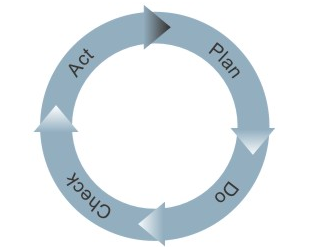
\includegraphics[scale=0.5]{ruben-tex/graphic/shewhartcycle}}
\caption{Shewhart cykeln \citep{Mindtools}}
\label{fig:shewcycle}
\end{figure}
\begin{enumerate}
  \item Planera. I detta skede ska målet fastställas, det vill säga sätta upp de krav som behövs för att kunden skall bli nöjd. Genom att göra detta är det tydligt om vad som skall göras och en överenskommelse finns mellan kund och leverantör. 
  \item Göra. När man konstaterat vad som behöver göras för att kunden skall bli nöjd är det dags att implementera ett sätt att arbeta och fullfölja processen.
  \item Studera. Efter att ha följt processen under en viss period är det dags att utvärdera om processen man har följt kommer leda till att man uppfyller de målen man har fastställt i planeringsfasen.
  \item Agera. Om man under studeringsfasen upptäcker att processen man följer inte kommer leda till att man uppfyller de krav som kund och leverantör var överens om måste detta åtgärdas omedelbart genom att planera om arbetsprocessen eller i viss mån diskutera kraven med kunden. Om processen som följs kommer uppfylla de krav som har satts upp kan man fortsätta med iterationerna av Shewhart cykeln precis som innan.
\end{enumerate}
\begin{figure}[h]
\centerline{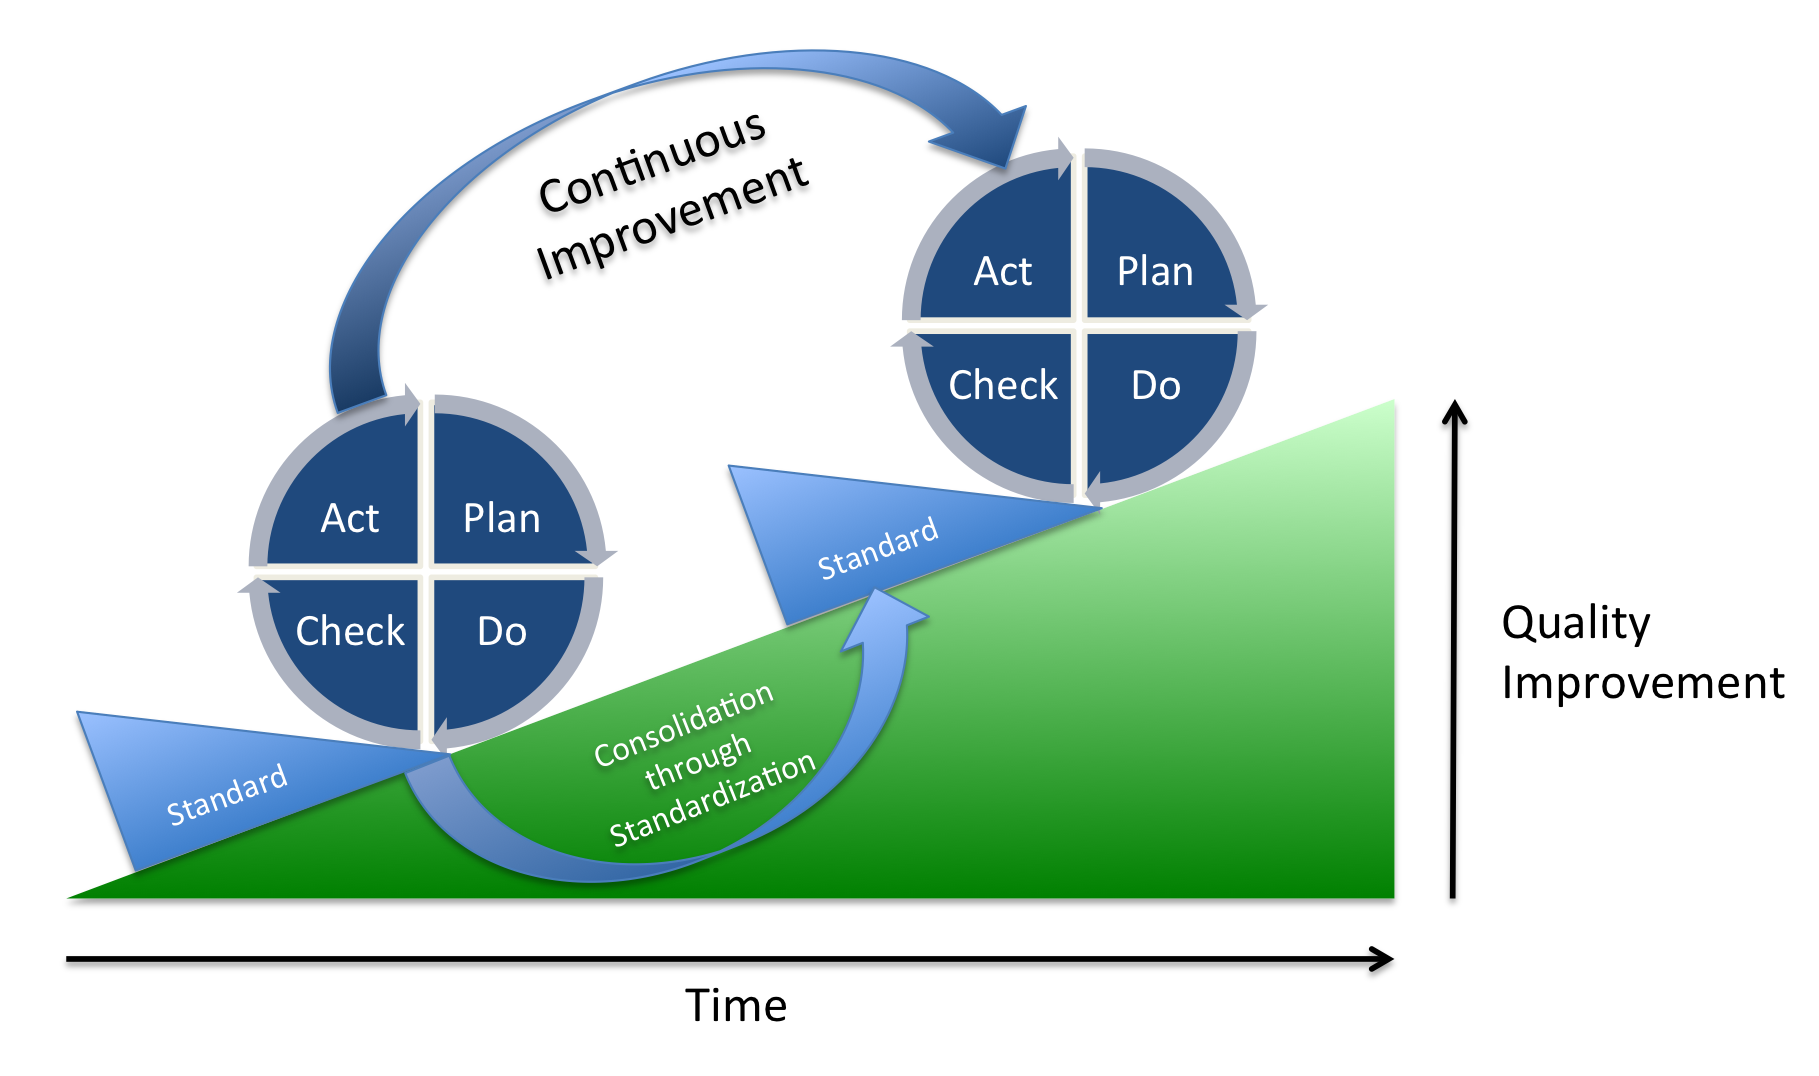
\includegraphics[scale=0.15]{ruben-tex/graphic/PDCA_Process}}
\caption{PDCA process \citep{Vietze}}
\label{fig:pdcaprocess}
\end{figure}
\noindent Genom att följa Shewhart cykeln under ett projekt kan man iterativt förbättra sin arbetsprocess och genom detta öka kvaliteten av den produkt man utvecklar, se figur \ref{fig:pdcaprocess}.
\newline
\newline
När det väl är dags för överlämning av en produkt eller tjänst är det bra att göra en kravinspektion innan. En kravinspektion enligt IEEE standarden för ''Software reviews'' syns nedan.

\begin{tcolorbox}[boxrule=1pt,leftrule=5pt,arc=0pt,auto outer arc]
\textbf{''}A process or meeting during which a software product is examined by a project personnel, managers, users, customers, user representatives, or other interested parties for comment or approval\textbf{''} \citep{SFSR}
\end{tcolorbox}

\noindent
Det man vill få gjort med en kravinspektion är alltså att produkten eller tjänsten som har tagits fram ska utvärderas av berörda parter så att den uppfyller de krav som har fastställts i ett tidigare skede för ett godkännande. En kravinspektion kan se ut som sådan \citep{Sandahl}:
\begin{enumerate}
\item{Tillträde.}
\item{Planering och översikt. Under detta steg sker en planering över hur inspektionen ska gå till och en översikt av produkten ges.}
\item{Individuell granskning. De berörda parterna granskar produkten eller tjänsten.}
\item{Möte. Efter granskningen görs en lista av alla de defekter som kan ha hittats.}
\item{Ändringar och uppföljning. I detta skede åtgärdar man de defekter som stöttes på och normalt brukar verifiera detta.}
\item{Utträde.}
\end{enumerate}

\subsection{Sammanfattning}
Sammanfattningsvis kan man konstatera att ett återkommande tema för att ta fram en högkvalitativ produkt eller tjänst är att planera, utföra och granska, för att sedan upprepa proceduren under projektets gång. Detta är dock bara en teoretisk tillämpning och verkligheten kan se annorlunda ut.

\section{Metod}
	För att ta reda på all information som behövs har ett flertal böcker blickats igenom. Ingen av dem har läst till 100\%, utan endast de intressanta delarna har läst med mer nogrannhet. För att verifiera att det som lästs stämmer har vissa delar testats i praktiken, i detta fall på projketet. Till exempel så har enhetstester körts på matris bibliotekts funktioner såsom matrisaddition, sytemtester och modultester har körts på den kvadratiska problem-lösaren och acceptanstester har körts på alla delar i projektet för att se till att alla krav är uppfyllda. Mer om detta kan läsas i resultat.
	
\subsection{Enhetstest}
	I ''Software Unit Testing'' \citep{ivv} definierar ett enhetstest som ett test på den minsta möjliga samlingen kod som fortfarande går att testa nyttofullt, alltså att koden är tillräckligt stor för att fel ska kunna uppstå. Dessa test är bra då de är riktade mot en så liten portion med kod och i och med detta sällan missar buggar och fel. Det som kan vara krångligt med enhetstest är att just hitta dessa minsta samlingarna med kod, speciellt om det är en extern part (en annan programmerare) som ska skapa och utföra testen. I och med att man kör enhetstester på så små delar av kod har de i teorin en tendens till att bli väldigt många om man ska täcka tillräckligt stor funktionalitet. Detta är dock oftast inget problem i praktiken eftersom många små funktioner ofta är triviala och har ytterst få uppgifter. Då behöver inte så många test skrivas, om ens ett enda.
\subsection{Modultest}	
	Det finns flera olika definitioner av vad en modul är, och i och med det blir det då svårt att definiera vad ett modultest är. I ''The Art of Software Testing'' definierar de att moduler och enheter är samma sak men jag har valt att istället gå efter Kristian Sandahls definiton. Han definierar att ett modultest är ett integrationtest utav två eller fler enheter. Det går ut på att man kombinerar ett antal enheter och sedan testar dem tillsammans. Testen i sig kan var väldigt lika enhetstest men täcker nu en mer komplex funktionalitet. Precis som enheter kan moduler vara svåra att definiera. Om allt för många enheter förs samman och modulen får mer funktionalitet kanske den till slut kan klassas som ett system, och då förlorar modultestningen sitt syfte. Om man har ett så litet projekt som detta så är moduldefinitionen ofta inte så svår, eftersom både komplexiteten och utvecklingsmöjligheterna är begränsade. Det är kritiskt vid dessa test att underliggande funktioner redan är testade. Om inte, kan i stort sett inga slutsatser, angående vad som är fel, dras när ett test misslyckas.
\subsection{Systemtest}	
	Ett systemtest är precis som modultest ett integrationstest, men nu utav ett antal moduler istället. Enligt ''The Art of Software Testing'' inriktar sig testet nu också vanligtvis på hela produkten som har utvecklats, för att se om funktionalitetskraven är uppfyllda. Detta för att säkerställa dess funktionalitet och för att hitta fel som uppstått vid kommunikation mellan moduler. Exempel på systemtest i vårt projekt är test av lösaren. Anledningen till att lösaren ses som ett eget system och inte är ihopbakad med GUI:t är att den ska kunna fungera separat. Givetvis är de båda ihopbakade också ett system, som också kräver systemtest.	
\subsection{Acceptanstest}	
	Ett acceptanstest är ett test som har målet att testa om programmet är acceptabelt. Med det menas att testen validerar ifall programmet uppfyller alla krav som ställs på det, och nu inte endast funktionalitetskraven. I vårt projekt är det huvudsakligen prestandan som behöver acceptanstestas. Då det prestandakrav produkten hade var relativt vagt ("Produkten ska ha likvärdig prestanda med Gurobi"), och att kravet sedan förhandlades bort, gjorde att testen inte hade så stor prioritet. Men för att få någon vetskap om produktens hastighet och för att garantera att kunden blir nöjd krävs ändå någon form utav test.
\subsection{Övrigt}	
	I projektet har även ett byggsystem använts, som smidigt kompilerat all kod automatiskt. Systemet har därefter även kört alla tester som skapats genom projektet.
	Med hjälp av byggsystemet och Kontinuerlig Integration har all kod då kunnat testas direkt när någon har skrivit ny kod och därav har det gått att se när och var feluppstått. Och eftersom systemet även har kört alla gamla test har koden säkerställts med att alla andra funktioner, de som inte har rörts, också fortfarande fungerar.
\section{Resultat}	
	Följande del beskriver hur arbetet med efterforskningen gick samt hur testen utfördes.
	\subsection{Efterforskning}
	Det finns otroligt mycket information om mjukvarutestning men samtidigt är ämnet ganska vagt då testning beror så mycket på just vad som ska testas. I vårt projekt visade det sig att ''Black Box''-testning var den metod som överlägset lämpade sig bäst. ''Black Box'' går ut på att man sätter en ''svart låda'' över det som ska testas, så att man endast kan se in- och utdatan. Sedan tittar man på utdata och ser ifall den är den förväntade. ''Black Box'' anses bra i detta projekt eftersom hela Quadopt är uppbyggd utav många små funktioner och resultateten som de ska ge tillbaka är oftast kända på förhand. Ett exempel på detta är matrisaritmetiken där resultatet, av till exempel en multiplikation, går att räkna ut ganska enkelt på papper. Enligt ''The Art of Software Testing'' ska dessa test utgå ifrån kravspecifikationen och andra dokument som beskriver vad produkten ska ha för funktionalitet. Boken beskriver också ''Black Box'' som en utmattande testteknik. Med det menar de att man borde testa alla möjliga indata till den svarta lådan och se så att svaren stämmer. Detta är precis som det står i boken i praktiken omöjligt. Speciellt i vårt projekt där det enda som begränsar antalet olika sätt en matris, bestående utav tal, kan se ut på är datorns minne. \newline
I projektet fanns dock ofta behovet av se en funktions lösningsgång, och då är ''Black Box'' en väldigt dålig metod. En metod som då lämpar sig bättre är ''White Box'' testning, som innebär att man tittar på den interna strukturen i en funktion. Därefter kan man se, efter vald indata, om lösningsgången är den väntade. I ''The Art of Software Testing'' står det att även denna metod kan problematisk då antalet lösningsgångar kan vara väldigt många. För att se om det ens är rimligt att utföra dessa test kan man se på funktionens cyklomatiska komplexitet. Cyklomatisk komplexitet innebär att man gör en graf över funktionen där de möjliga stadierna i lösningsgången är noder, och de möjliga lösningsvägarna är bågar. I ''Structured testing'' \citep{structest} står det att om denna komplexitet är för stor ökar antalet fel som programmeraren gjort väldigt fort, och samtidigt blir det i stort sett omöjligt att utföra några ''White Box''-test då fel kan uppstå på så många ställen. \\ 	
För att säkerställa projektets krav behövdes bara en testmetod till, och det var en metod för att mäta prestanda. Den som valdes var ''Load testing'' som innebär att man belastar programmet med mycket data och ser hur bra det fungerar. I projektets fall gavs lösaren många problem och tittade på hur fort det gick i förhållande till andra lösare. \newline	
Det skulle kunnat varit så att GUI:t hade haft högre prioritet än vad det hade. I det fallet hade olika typer av UX- och användartest varit nödvändiga för att kvalitetssäkra produkten. Men eftersom GUI:t beställdes utifrån kundens personliga behov, var det tydligt definierat redan från början att det var av låg prioritet. 
	
	\subsection{Praktik}
	Som beskrivet tidigare finns det i stort sett oändligt många kombinationer av in- och utdata.	För att då kunna utföra ''Black Box''-testerna behövdes antalet testfall reduceras. Detta åstadkoms genom att ha möten med kunden som klargjorde att indata till programmet alltid skulle vara giltig. Det reducerade antal testfall enormt mycket, men som beskrivet i resultatet av efterforskningen finns det även väldigt mycket giltig indata. Exempelvis för matrisaritmetiken. Dessa test gick också att reducera genom att de flesta operationer är triviala och endast kräver numeriska test såsom nolldivision och flyttalsfel. Genom att även utnyttja ''White Box''-tekniken gick det att utforma olika ''Black Box''-test som tog olika vägar genom koden och på så sätt bara skapa ett test för varje väg. Denna teknik utnyttjades endast på mindre funktioner såsom moduler för att antalet olika fall skulle begränsas till något som var rimligt. \newline
	För lösaren gick det att applicera samma metod, eftersom dess funktionalitet bygger mycket på underliggande funktioner. Det som skilde sig gentemot småfunktionerna var att nu behandlades oftast rader eller kolumner i matriser istället för enskilda element. Detta ledde till att de flesta test kontrollerade på kanterna utav det tillåtna området. Alltså kunde ett test vara att försöka hämta ut en radvektor på rad -1 ur en matris, vilket skulle vara ogiltigt.\newline
Vid granskning av testresultat från Git, Travis (verktyg för Kontinuerlig integration) och gruppmedlemmar visade det sig att majoriteten fel av bestod utav två typer: ''Assertion''s som misslyckats och ''Segmentation fault''. En ''Assertion'' är ett test inuti koden som avbryter exekveringen om testet inte går bra. ''Segmentation fault'' är ett programmeringsfel som resulterat i en ogiltig läsning eller skrivning till minnet. Felen som uppstod var väldigt utspridda och olika. Det som de flesta hade gemensamt var dock att de låg på en låg nivå, alltså i bottenfunktionerna. \newline	
	För att testa algoritmens hastighet stötte gruppen på oväntade problem, lösarna var för snabba.	Då varje testkörning tog 0.00 sekunder för alla lösarna förutom MATLAB behövdes testen köras många gånger för att se en tydlig skillnad. Anledningen till att MATLAB är långsammare är för att den är oerhört generell men förmodligen inte gjorts med fokus på att vara snabb. Gurobi är snabb eftersom dess enda uppgift är att lösa sådana här problem och har arbetats på under lång tid. Vår algoritm är snabb eftersom den inte är generell, alltså bryr vi oss inte om vissa specialfall som vi aldrig kommer stöta på. \newline
	För att då testa deras prestanda fick lösarna lösa olika optimeringsproblem många gånger, ofta upp emot 1000 gånger, för att kunna skilja deras egentliga hastighet. Att köra testen på vår lösare och i MATLAB var enkelt då vi hade funktionalitet för att konvertera matriser från MATLABs definition till vår, och vice versa. Däremot så var det krångligare i gurobi eftersom tiden som var allokerad för utbildning av programmet var begränsad. Det tvingade gruppen till att mata in problemet på ekvationsform vilket gjorde att gruppmedlemmarna var tvungna att köra endast små tester. Redan vid problem med fler än 10 bivillkor skulle det ta väldigt lång tid att konvertera och mata in problemet. \newline
	
	
	\subsection{Enhetstester}
	Under projektet har många enhetstest skrivits (framförallt för matrisbiblioteket). Dessa test har skrivits innan och under kodningen och sedan utförts direkt efter att koden blivit klar. Det som var intressant med dessa test var mängden av fel som upptäcktes direkt. Det ledde till att utvecklingen blev mycket effektiv då fel kunde åtgärdas direkt.
	
	\subsection{Integrationstester}
	De modultester som planerades och utfördes under projektet var framförallt lösarens funktioner. Modulerna var uppbyggda utav sammansättningar av enheter från matrisbiblioteket och andra strukturer. Dessa test utfördes vanligtvis samtidigt som implementeringen pågick. Detta för att hela tiden se till att rätt protokoll och gränssnitt användes.\\
De systemtester som utförts är tester utav lösaren och subproblemslösaren. Dessa ansågs vara tillräcklig komplexa för att ses som system. 
	
	
	\subsection{Acceptanstester}
	De acceptanstester som utförts under projektet är framförallt prestandatester. Detta då det enda kravet lösaren hade var att den skulle vara ungefär lika snabb som den kommersiella lösaren Gurobi. Då detta krav sedan togs bort lade mindre energi på prestandatester. Men de delar som ändå testats var framförallt underfunktioner till lösaren, såsom matrisbiblioteket och subproblemslösaren.
	
	\subsection{Misstag}
	Det hände att vissa modul- och systemtester skedde innan de underliggande enheterna blivit testade. Ett exempel på det är lösaren, som gruppen ivrigt ville få igång och började därför testa den tidigt. Då den inte fungerade korrekt gjorde detta att det tog lång tid att hitta felen som förmodligen hade upptäckts mycket snabbare om bara rätt testprocess hade använts.
	
	
\section{Diskussion}
Under denna del kommer en diskussion angående om resultaten ske samt metoderna som användes.
\subsection{Resultat}
Resultaten för alla tre punkter måste anses vara rimliga. Den första punkten angående vad som är rätt nivå är en väldigt diffus fråga och kan bara svaras genom att båda parter, dvs leverantör och kund har ett enhetligt svar. Eftersom det man kommer överens om i en eventuell kravspecifikation måste räcka att fullfölja för att det ska klassas som rätt nivå gällande kvalité. Sen om kunden hade velat haft några andra funktioner med produkten eller tjänsten så borde kunden ha specificerat detta. Leverantörer har också skyldighet att försöka uppfylla alla krav som har specificerats på ett snyggt sätt och inte bara slänga ihop något som fungerar, små detaljer kan utmärka ett arbete.
\newline
\newline
Den andra punkten finns det inte mycket att diskutera om, som allt annat i livet krävs det struktur för att man ska uppnå något. Under teoridelen i kapitel tre kan man konstatera att planera, utföra och granska antagligen kommer generera en produkt eller tjänst av tillräckligt god kvalité.
\newline
\newline
Angående den sista punkten kan man byta svaret från ett ja till ett nej, då ett krav förhandlades bort. I detta projekt hade kandidatgruppen endast ett mätbart krav, detta krav specificerade att optimeringsalgoritmen skulle vara likvärdig i hastighet i jämförelse med en kommersiell mjukvara kallad ''Gurobi''. ''Gurobi'' specialiserar sig i att lösa olika sorters optimeringsproblem \citep{gurobi}. Under projektets slutskede diskuterade kandidatgruppen med kunden om att det kommer bli svårt att vara jämbördig med ''Gurboi'', detta var inget problem för kunden och kravet kunde tas bort. Kunden tryckte på att det viktigaste var att koden fungerar och att den är väldokumenterad, vilket den är. Däremot kan jag tycka att om man tar bort ett krav så har man misslyckats och därför anser jag att man kan ändra svaret till nej, slutprodukten håller inte tillräckligt god kvalité, men då är jag väldigt hård mot mig själv och kandidatgruppen. Däremot säger teorin bakom det hela att produkten håller tillräckligt god nivå då den uppfyller alla krav, det ska inte spela någon roll om man har förhandlat bort något krav eller inte.

\subsection{Metod}
Efter slutförandet av projektet och analys av hur det hela gick finns det många saker man hade kunnat gjort annorlunda. Ett återkommande problem som stöttes på under projektets gång var att kodstandarden som hade satts upp från början inte följdes helt och hållet, inte förens den sista iterationen skrevs kod efter den. Detta resulterade i att mycket tid lades ner på att refaktorera kod. Kodstandarden innehöll inte heller allt som bör ta hänsyns till. Ett exempel är att frigöra minne, vilket resultera i att mycket tid lades ner på att hitta och åtgärda minnesläckor. Eftersom kandidatgruppen hade ett krav på att skriva pålitlig kod så är förstås minnesläckor inte accepterbart. 
\newline
\newline
Jag tror att slutprodukten skulle ha sett annorlunda ut om kodstandarden täckte fler områden i hur man ska skriva kod samt om man tryckte på hur viktigt det är att följa kodstandarden. Jag som kvalitetsamordnare hade kunnat trycka mer på att kodstandarden skall följas för att en produkt av bättre kvalité skulle skapats.
\newline
\newline
I teoridelen visade forskningen att om man ska uppnå en högkvalitativ produkt kan man t.ex. använda sig av Shewhart cykeln, planera, göra, studera och agera. Kandidatgruppen planera hur man skulle skriva kod, man följde inte kodstandarden, kandidatgruppen var väl medveten om det. Vid detta stadiet borde man agera, visserligen sas det åt folk att börja använda kodstandarden, men det hade nog varit bättre att utvärdera om kodstandarden och föra dialog om varför den inte följs för att skriva en ny som möjligtvis alla känner sig bekväma med.

\section{Slutsatser}
{\LaTeX} lämpar sig mycket väl för teknisk dokumentation i ett programmeringsprojekt. Denna slutsats kan dras från det {\LaTeX} dokument gruppen har producerat. {\LaTeX} gav oss verktygen för att infoga figurer, matematiska formler, ekvationer, algoritmer och pseudokod som behövdes för dokumenten i projektet.   
\newline
\newline
Det tog hela projekttiden för att samtliga medlemmar skulle känna att de behärskade {\LaTeX}. Detta kan ses som en lång inlärningskurva för språket och att det tog onödig tid från andra delar av projektet. Dock var detta aldrig egentligen något problem, mycket hjälp fanns att hämta från internet och då två av gruppmedlemmarna behärskade {\LaTeX} sedan tidigare kunde de hjälpa och lära resten av gruppen. 
\newline
\newline
Om ingen av gruppens medlemmar hade använt {\LaTeX} sedan tidigare kan det diskuteras om det hade varit lönsamt för gruppen att lära sig det. Då hade mer tid behövts läggas på utbildning av språket och andra uppgifter hade fått lida. Som sagt lämpar sig {\LaTeX} mycket väl för teknisk dokumentation i ett programmeringsprojekt och även om det hade tagit mer tid så hade det varit värt i det långa loppet.    
\newpage
\setcounter{secnumdepth}{0}
\section{Kodstandard}

\lstset{ language=C, backgroundcolor=\color{black!5}, basicstyle=\footnotesize}

\begin{itemize}
  \item Indentering sker med två blanksteg.
  \item Funktionsnamn och variabelnamn skrivs med små bokstäver med understreck som separerator mellan ord. Får heta vad författaren önskar så länge det är relevant. 
  \item Pekare skrivs med asterisken direkt efter datatypen.
  \item Filer inkluderas där de behövs, antingen i c- eller h-filen.
  \item Den öppnande måsvingeparentesen skrivs på samma rad som funktionsnamnet och returtypen. Den stängande parentesen skrivs ensam på raden efter den avslutande satsen i funktionen. If-satser och liknande skrivs på samma sätt.
  \item Typedef sker separat från struct-deklarationer.
  \item Kommentarer skrivs som i exemplet nedan.
  \item Koden skall vara skriven på engelska.
\end{itemize}

\begin{lstlisting}
/*
  Author: Alexander Yngve
  Date: 2015-02-11
  Description: Short description of why this file is needed.
*/

#include <stdio.h>

/* Short explanation of why this type is needed. */
struct struct_t{
  int* pointer;
  int number;
};

typedef struct struct_t struct_t;

/* Short explanation of why this function is needed. */
int main(){
  printf("Hej\n");

  struct struct_t data_1;
  data_1.number = 4;
  printf("%i\n", data_1.number);

  struct_t data_2 = {NULL, 5};
  printf("%i\n", data_2.number);

  return 0;
}
\end{lstlisting}



\newpage

\resumecontents[default]
\addcontentsline{toc}{section}{Referenser}
\bibliography{tex/refs}{}
\end{document}
